\documentclass{memoire}
\begin{document}
\renewcommand{\bibsection}{\section*{Bibliographie}}

% ORGANISATION GENERALE
% Le mémoire comprend une partie principale de synthèse, nécessairement courte, complétée par un dossier d’analyses détaillées. 
% Rédiger la synthèse vous conduit à mettre en cohérence vos études et travaux, et à rendre accessible au jury, sous un format clair et rapidement lisible, l’essentiel de votre travail. 
% Les analyses détaillées sont un récapitulatif de vos travaux : études, comptes-rendus, expérimentations et lectures faites en cours d’année.

% PARTIE SYNTHESE
% Son introduction résume de manière succincte l'origine du questionnement initial et explique le titre du mémoire. Elle introduit et justifie le plan du mémoire, en indiquant bien dans quelle partie la problématique est définie et justifiée. Dans le cas d’un mémoire préparé à deux ou à trois, elle explicite par ailleurs comment vous avez collaboré pour rédiger le mémoire à plusieurs (synthèse et analyses). 
% La synthèse doit comprendre une partie de définition et une justification de la problématique, qui s'appuie sur une synthèse argumentée de ce qui vous y a conduit: vos lectures d'une part, et d'autre part certaines de vos observations ou expérimentations.
% Elle décrit et justifie également le corpus permettant de répondre à la problématique ou de la faire évoluer: entretiens, analyses de documents (manuels, copies, …), observations, construction de séances / séquences, expérimentations en classe, notes de lecture.
% Elle aboutit à un résumé de vos principales conclusions et propose des perspectives pour développer le travail engagé, en termes de nouvelles lectures, de poursuite d'étude (formations, diplômes certifications envisagées..) ou de valorisation de votre travail.
% Elle inclut une bibli- et sitographie aux normes et commentée pour les références les plus importantes (2-3 lignes de commentaire pour les lectures qui vous ont le plus servi).
% Longueur de l’ordre de 15 à 20 pages pour un mémoire individuel, 25 à 30 pages en binôme ou trinôme. 
% Police et espacement, pour toute partie dactylographiée: Times 12 pt, interligne 1,5.

% la page de garde comporte les éléments et mentions suivants: 
% le logo de l'ESPE de Créteil (obligatoire) + logo de votre université d'inscription (facultatif)
% "MÉMOIRE de MASTER MEEF 2nd degré, parcours mathématiques. Année 2018-19"; 
% Vos noms et prénoms; 
% Le titre du mémoire; 
% Le nom du ou des responsable(s) de suivi de mémoire; 
\begin{titlepage}
    \begin{center}
        \includegraphics[scale=0.5]{logo_UPEC_ESPE.png}

        MEEF 2\up{nd} degré, parcours Mathématiques

        Année 2018-19 UE d'accompagnement de stage

        \vspace*{\fill}

        \Huge{Différenciation et autonomie : quelles méthodes pour quels résultats ?}

        \vspace*{\fill}

        \begin{tabular}{ccc}
            \Large{Henriette, Julia}&\Large{Jidouard, Xavière}&\Large{Milis, Victoire}
        \end{tabular}

        \vspace*{\fill}

        \Large{Responsable de suivi de mémoire : Grapin, Nadine}

        \vspace*{\fill}
    \end{center}
\end{titlepage}


% Tous les mémoires doivent comporter un résumé de 200 à 250 mots et une liste de 5 mots-clés.
% la deuxième page comporte les éléments et mentions suivants:
% Un résumé de 300 à 500 mots. Il indique le contexte du mémoire, résume sa problématique et ses principales conclusions. (Contradiction avec le cadrage Mahara)
% Les autorisations de diffusion, sous la forme suivante: 
% J'autorise l'ESPE:
% à exploiter le texte de mon mémoire dans la formation des étudiants MEEF  [OUI / NON] 
% à communiquer mon nom et mes coordonnées à de futurs étudiants MEEF qui souhaiteraient me contacter au sujet de mon mémoire [OUI / NON]
\begin{abstract}
Ce mémoire rassemble les réflexions et expérimentations de 3 professeurs stagiaires
à propos de différentes méthodes de différenciation. Le but de ces méthodes
étant d'avoir des techniques applicables généralement, en non spécialisées sur
certaines séquences.
\paragraph*{}Le mémoire présente dans un premier temps la découverte de la notion de différenciation pédagogique et le choix d'orienter la problématique vers l'autonomie des élèves, et ce à travers les lectures effectuées au cours du stage.\\
Les auteurs y justifient ainsi leurs choix de pratiques en répondant aux questions telles que « \textit{Pourquoi différencier ?} », « \textit{Que signifie différencier ?} », « \textit{Quelles pratiques pouvons-nous raisonnablement expérimenter lors de l'année de stage ?} », « \textit{Comment mesurer l'impact des pratiques expérimentées ?} ».\\ 
Les différents choix de pratiques pédagogiques sont ensuite expliqués puis détaillés dans des parties individuelles. Le document comporte enfin une analyse croisée des expérimentations effectuées par chacune, ainsi que l'état des réflexions des auteurs et les difficultés rencontrées par celles-ci autour des pratiques de différenciation pédagogique et de mise en autonomie des élèves.\\
Le but commun entre les réflexions et expérimentations est de rendre les élèves
plus autonomes tout en leur proposant une acquisition des compétences différenciée, sur différents degrés.
\end{abstract}

Mots-clés : \textbf{différenciation}, \textbf{méthodes}, \textbf{autonomie}, \textbf{pédagogie}, \textbf{tutorat}, \textbf{évalutations différenciées}, \textbf{parcours différenciés}, \textbf{supports différenciés}

\vfill
\section*{Remerciements}
Nous tenons à remercier Nadine Grapin d'avoir encadré ce mémoire et pour l'intérêt qu'elle a porté à nos pratiques pédagogiques de manière générale.\\
Merci également à nos tuteurs de l'ESPE respectifs, Alain Bernard et Marie-Hélène Le Yaouanq pour leur enseignement et leurs bons conseils tout au long de cette année. De même, nous remercions nos tutrices terrain \remark{mettre le nom des tutrices dans l'ordre alphabétique ici} Marine Doceul, Claire Hizembert pour leur accompagnement dans nos établissement et pour tout ce qu'elles ont apporté à l'amélioration de nos pratiques.\\
De manière générale nous tenons à remercier les collègues formateurs de l'ESPE et de nos établissements respectifs pour leur bienveillance et pour avoir pris le temps de nous aider à nous améliorer.\\
Nous remercions enfin nos proches pour nous avoir soutenues lors de cette année de stage et dans notre projet d'enseignement.
\vfill
Nous autorisons l'ESPÉ :
\begin{itemize}
\item à exploiter le texte de notre mémoire dans la future formation des étudiants MEEF : \textbf{\textsc{Oui}} ;
\item à communiquer notre nom et coordonnées à de futurs étudiants MEEF qui souhaiteraient nous contacter au sujet de notre mémoire : \textbf{\textsc{Oui}}.
\end{itemize}


% La troisième page comporte le sommaire de la synthèse et inclut la liste des analyses détaillées.
\include{sections/toc}

% Le corps de la synthèse ne dépasse pas 30 pages et est organisé en parties et sous-parties lisibles.

% De l’ordre de 1 à 2 pages 
% Elle résume de manière succincte l'origine du questionnement initial et explique le titre du mémoire.
% Elle introduit et justifie le plan du mémoire, en indiquant bien dans quelle partie la problématique est définie et justifiée. 
% Elle explicite par ailleurs comment vous avez collaboré pour rédiger le mémoire à plusieurs (synthèse et analyses).
% La rédaction permet d'identifier les parties rédigées collectivement ou individuellement; les choix que vous avez faits pour organiser entre vous la rédaction, sont indiqués en introduction.
\section{Introduction}
%Ceci est une phrase qui fait référence à la bibliographie\cite{bibliotest}.

\textit{<- Début du bilan d'étape ->}

Ayant chacune un parcours différent, nous nous sommes retrouvées autour d’un même constat suite à la prise en main de nos classes : le mode de fonctionnement habituel de nos classes ne nous permet pas de répondre aux besoins spécifiques de nos élèves et de leur donner les moyens de travailler correctement en autonomie. Sur les conseils de nos tuteurs terrain, nous avons décidé de profiter du travail sur le mémoire pour chercher un mode de fonctionnement ou des solutions spécifiques à notre public. Nous nous sommes rapidement tournées vers le thème de la différenciation pédagogique, en ayant une connaissance quasi nulle sur le sujet.

La première étape de notre démarche a donc été de nous renseigner auprès de Nadine Grapin, notre directrice de mémoire, qui nous a orientées vers des lectures et des premiers axes de réflexion sur le sujet : quels objectifs ? Quelle(s) forme(s) de différenciation ? 

Suite à différents échanges avec nos encadrants et nos collègues et après une première série de lectures, nous avons choisi d’orienter le sujet de notre mémoire vers la différenciation pédagogique dans le but de rendre les élèves autonomes. Ce choix commun est lié à des motivations différentes pour chacune d’entre nous. 
Le cheminement de nos réflexions sera développé dans la première partie de ce document, où nous ferons l’état des lieux des travaux menés sur la période de novembre et décembre et où nous détaillerons les pistes de réflexion qui en sont ressorties.
Dans une seconde partie, suite au bilan que nous viendrons de dresser, nous listerons les pistes de travail que nous envisageons de suivre. Il sera notamment question des lectures envisagées, des mises en pratiques de procédés rencontrés lors de nos recherches et les problématiques de mise en place associées.

Nous développerons en troisième partie notre mode de fonctionnement actuel et l’organisation prévue des pistes identifiées en seconde partie.
Nous terminerons enfin par les retours que nous avons reçus suite à la présentation orale du bilan d’étape du 16 janvier 2019. 

\textit{<- Complément issu du bilan d'étape ->}

Suite aux différents entretiens que nous avons pu avoir avec Nadine Grapin et aux retours que nous avons eu suite à notre présentation du 16 janvier, nous avons eu de nouvelles réflexions : 
\begin{itemize}
    \item avons-nous une problématique ou plusieurs problématiques ? La réponse à cette question nous permettra de structurer notre mémoire.
    \item quelle est la place de la différenciation par rapport à l’autonomisation ? Nous avons un double objectif : celui de rendre les élèves autonomes pour pouvoir mieux gérer la classe et pouvoir consacrer plus de temps aux élèves en ayant besoin, et celui de différencier, à savoir fournir aux élèves une manière d’accéder aux compétences qui prend en compte leurs points forts et points faibles.
\end{itemize}
    
Nous nous sommes aussi rendues compte que nous faisons déjà plus de différenciation que nous le pensions (voir tableau en annexe) : nous avons tendance à construire le cours avec les élèves, mettre en place des méthodes non expertes avec les élèves, tout en fournissant des méthodes expertes aux élèves qui voudraient les utiliser.

De plus, cet entretien a permis à Julia de mieux formuler sa problématique qui s’avère être de trouver une pratique (le parcours différencié) s’appuyant sur l’autonomie des élèves pour mieux différencier. La présentation orale du parcours différencié a par ailleurs permis de mettre en avant des points de réflexion supplémentaires : quels exercices corriger ? Quels exercices sont obligatoires? Comment évaluer la progression des élèves et pour quoi ? Que faire une fois l’évaluation effectuée ?

\textit{<- Fin du bilan d'étape ->}

% La synthèse doit comprendre une partie de définition et une justification de la problématique, qui s'appuie sur une synthèse argumentée de ce qui vous y a conduit: vos lectures d'une part, et d'autre part certaines de vos observations ou expérimentations.
% Elle décrit et justifie également le corpus permettant de répondre à la problématique ou de la faire évoluer: entretiens, analyses de documents (manuels, copies, …), observations, construction de séances / séquences, expérimentations en classe, notes de lecture.
\section{Synthèse de notre réflexion}
Dans cette partie, nous développons la construction de notre problématique à travers les principales questions soulevées par nos lectures. Celles-ci nous ont permis de structurer notre réflexion autour de la notion de différenciation pédagogique :

\begin{itemize}
  \item Que signifie différencier ?
  \item Pourquoi différencier ?
  \item Quelles pratiques pouvons-nous raisonnablement expérimenter lors de l'année de stage ?
  \item Quelles sont les erreurs à ne pas commettre lors de nos expérimentations ?
  \item Comment mesurer l'impact des pratiques expérimentées ?
\end{itemize}

Cette section ne suit pas l'ordre des questions ci-dessus. Il est en effet important pour nous que le lecteur comprenne d'abord pourquoi nous avons choisi de travailler sur des méthodes de différenciation et comment nos lectures nous ont confirmé ce choix, avant de donner une définition précise de ce qu'est la différenciation pédagogique.\\
Après avoir défini pourquoi différencier, nous développons la définition de différenciation pédagogique, ainsi que les pratiques que nous avons envisagées au fil de nos lectures et des entretiens avec nos collègues. Nous abordons ensuite les difficultés que nous avons anticipées pour les pratiques pédagogiques que nous souhaitions mettre en place. Enfin, nous introduisons les premiers questionnements autour de la mesure de l'impact de nos pratiques sur l'autonomie des élèves et l'acquisition des compétences.\\

\subsection{Pourquoi différencier ?}

%\remark{D'après la carte mentale, on devrait retrouver ici la remédiation, rendre les élèves autonomes et faciliter la gestion de classe.}

Lorsque nous avons commencé ce mémoire, nous avions une vision partielle de ce qu'était la différenciation pédagogique. Ce sont nos lectures sur les recherches autour de la notion et des pratiques associées à cette notion qui nous ont confirmé le choix de notre sujet de recherche, et surtout l'objectif de notre travail.
\paragraph{} Une des richesses de notre trinôme est que nous avons chacune un parcours professionnel et des profils de classe différents (dont établissement REP et évaluation par compétences). Cela nous permet d'avoir des échanges intéressants sur ce que nous pouvons rencontrer dans les différents environnements, comment nous abordons les difficultés qui se posent à nous\ldots \\
Malgré nos différences, nous avons toutes eu le même constat à la rentrée : chacune d'entre nous rencontrait des difficultés de gestion de classe lorsqu'elle souhaitait consacrer du temps à des élèves ayant besoin d'une aide dédiée. Nous avons toutes eu le sentiment que les pratiques que nous connaissions (pour les avoir expérimentées en tant qu'élèves) ne suffisaient pas à répondre à notre besoin de fournir un accompagnement personnalisé à nos élèves.\\
Le sujet de différenciation pédagogique proposé par Nadine Grapin dans le cadre du master MEEF de l'UPEC semblait proposer des pistes de réflexion en adéquation avec notre problématique.\\
Sur ses conseils, nous avons lu les documents du Cnesco\footnote{Conseil national d'évalution du système scolaire} produits dans le cadre de la conférence consensus sur la différenciation pédagogique nous ont donné un tout nouvel éclairage sur la notion de différencation pédagogique.
\paragraph{}En particulier, l'article d'Alexia Forget\cite{cnesco_etat_lieux} présente l'état de la recherche autour de la différenciation pédagogique avec une attention particulière à la définition de la notion, mais aussi au « pourquoi » \footnote{Reconnaître la diversité des élèves ? Mettre en valeur cette diversité ? Par devoir ethique ?} et au « pour quoi » \footnote{Quelle finalité ?} différencier.\\
Suite à la lecture de ce document nous avons échangé sur nos situations respectives et sur ce que nous souhaitions pour nos élèves. Il est revenu que nous étions bloquées par l'incapacité de nos élèves à travailler en autonomie, c'est à dire d'effectuer intégralement un travail individuel sans aide et spontanément\footnote{sans forcément réussir le travail dans sa totalité}. Nous avons donc décidé d'orienter notre travail sur l'expérimentation et l'analyse de pratiques pédagogiques de différenciation dans le but de rendre nos élèves plus autonomes, tout en leur proposant un travail adapté à leurs besoins.\\
Nos objectifs finaux se sont dessinés au fil des lectures sur l'autonomie\cite{Meirieu_autonomie}\cite{ilots_bonifies} et de nos échanges. Après un bilan d'étape avec Nadine Grapin, nous nous sommes interrogées sur la place de la différenciation par rapport à l’autonomisation dans notre travail de recherche. Il est apparu que nous n'avons pas toutes les trois le même objectif final :
\begin{itemize}
	\item Victoire a validé ce choix suite à ses propres recherches sur le travail de groupe, qu’elle souhaitait établir dans ses classes de 6\up{e} et 4\up{e}. L’intérêt est notamment pour elle d’explorer la pratique du tutorat par les élèves et les ilots bonifiés.
	\item Pour Xavière, qui enseigne en collège REP (5\up{e}, 4\up{e} et 6{e} en AP\footnote{Accompagnement Personnalisé}),  le premier objectif en début d'année était de rendre les élèves autonomes en classe pour avoir plus de temps à consacrer à l’accompagnement personnalisé des élèves et passer d’une gestion de classe globale systématique à une gestion de classe plus ponctuelle. Plus tard dans l'année un second objectif s'est dégagé : donner à tous les élèves les outils nécessaires à un travail hors classe autonome. Sa tutrice ESPÉ (Marie-Hélène Le Yaouanq) a validé ce choix, en cohérence avec les observations effectuées lors de visites et avec les contenus de cours déjà proposés.
	\item  Julia cherche à habituer ses élèves à travailler de manière autonome sur des dispositifs de travail différenciés. L'objectif final est de réduire les écarts de niveau dans ses classes de 6\up{e} et 5\up{e}, en limitant son intervention lors des phases d’exercices pour accompagner les élèves nécessitant une assistance personnalisée.
\end{itemize}
  Nous avons cependant un double objectif commun : celui de rendre les élèves autonomes pour pouvoir mieux gérer la classe et pouvoir consacrer plus de temps aux élèves en ayant besoin, et celui de différencier, à savoir fournir aux élèves une manière d’accéder aux compétences qui prenne en compte leurs points forts et leurs points faibles.


\subsection{Qu'est-ce que c'est la différenciation ?}
Comme indiqué dans la partie précédente, c'est à la lecture de l'article d'Alexia Forget\cite{cnesco_etat_lieux} que nous avons pris conscience de ce qu'est la différenciation pédagogique. La définition la plus pertinente est, selon nous, celle donnée par Eduscol\cite{Eduscol} : \og La différenciation pédagogique consiste à mettre en \oe{}uvre un ensemble diversifié de moyens
et de procédures d’enseignement et d’apprentissage pour permettre à des élèves d’aptitudes
et de besoins différents d’atteindre par des voies différentes des objectifs communs.\fg{}.\\
Nous avons retrouvé dans ces lectures et dans d'autres ressources\footnote{En particulier, Dominique Lafontaine\cite{cnesco_Lafontaine} traite ainsi de la différenciation dans le système éducatif}, les différents types de différenciation pédagogiques pouvant être mises en place (différenciation successive, différenciation simultanée) ainsi que des exemples de pratiques de différenciation (exercices avec variables didactiques différentes selon les élèves, variation des supports, variation des procédures, organisation spécifique de la classe par groupes, prédagogie inversée\ldots).
\paragraph{}Nous nous sommes aussi rendues compte que nous faisons déjà plus de différenciation que nous le pensions (voir tableau en annexe \ref{tableau_differenciation}) : nous avons tendance à construire le cours avec les élèves, mettre en place des méthodes non expertes avec les élèves, tout en fournissant des méthodes expertes aux élèves qui voudraient les utiliser.\\
Nous n'avons pas axé nos recherches sur un type de différenciation en particulier mais avons recherché des pratiques pédagogiques que nous pourrions expérimenter en classe. De ce point de vue, il existe une documentation riche sur la variété des pratiques ou les modalités de différenciation. Nous citerons en particulier les notes et recommandations des experts ayant contribué à la conférence \og Consensus \fg{} du Cnesco\cite{cnesco_notes_experts}\cite{cnesco_synthese}, les travaux publiés par l'\textsc{Ifé}\footnote{Institut français de l'éducation} \cite{ife}, les publications de l'inspection académique de Créteil\cite{IPR_math_mouvement}.
\paragraph{} Nous avons ainsi découvert une quantité importante de documents abordant la différenciation pédagogique de manière théorique, soit de manière générale, soit sur un axe spécifique (« Différencier avec les TICE\footnote{Technologies de l'Information et de la Communication pour l'Éducation} », « Différencier sur une évaluation en mathématiques », etc.).\\
Ces lectures nous ont permis de sélectionner une pratique pédagogique adaptée à nos classes et répondant a priori à notre problématique parmi un large choix de dispositifs. Comme nous allons le voir par la suite, l'anticipation de certaines difficultés ou de pièges à éviter a joué sur notre choix final.


\subsection{Quels sont les écueils à éviter ?}
%à caser
En plus de nous donner des pistes de pratiques, nos lectures nous ont également donné des indications sur les erreurs à éviter comme :
\begin{itemize}
	\item se focaliser sur les élèves en difficulté et réduire la différenciation pédagogique à un travail de remédiation\cite{Eduscol}\cite{renc_pedago}
	\item transformer les séances de différenciation en temps d'accompagnements personnalisés\cite{Eduscol}
	\item expérimenter une pratique pédagogique de manière ponctuelle, indépendamment de la séquence travaillée\cite{renc_pedago}\footnote{La pratique de différenciation pédagogique doit au contraire s'inscrire de manière cohérente dans un cycle d'apprentissage des élèves.}
	\item ne porter la différenciation que sur un type de dispositif. Nous avons vu que nous pratiquions déjà plusieurs formes de différenciation dans nos classes, l'objectif est donc de continuer d'enrichir nos pratiques.
	\item différencier pour différencier. Tout dispositif de différenciation doit avoir un objectif clair et atteignable par les élèves\cite{Eduscol}\cite{Meirieu_différenciation}\cite{cnesco_notes_experts}
\end{itemize}
En choisissant les dispositifs de différenciation que nous souhaitions travailler dans le cadre du mémoire, nous avons pris en considération ces avertissements, tout en anticipant d'autres difficultés. Cela nous a fait formuler les questions suivantes :
\begin{itemize}
	\item quelles pratiques peut-on raisonnablement mettre en place pour effectuer une différenciation ? Nous manquons de temps et d’expérience, nous ne pouvons pas différencier chaque exercice ou point de cours ;
	\item sur quelles modalités pouvons nous différencier ? Le plus classique reste les variables didactiques dans un même exercice, un autre que des collègues utilisent déjà est un parcours différencié d’exercices, réactif aux erreurs commises\ldots Il est aussi possible de faire de la différenciation au niveau des supports mis à disposition des élèves, mais là aussi, cela demande beaucoup de temps à mettre en \oe{}uvre.
\end{itemize}

\paragraph{}Suite à nos recherches et aux échanges effectués sur nos pratiques et nos besoins, Victoire a choisi d’axer ses recherches autour des permis de tutorat pour les élèves et des ilots bonifiés. De son côté, Xavière a préféré s’orienter vers une différenciation au service de la création d'outils pour faciliter l'autonomie et l'auto évaluation de ses élèves. Julia a, quant à elle, d’abord opté pour la mise en pratique d’un parcours d’exercices adapté à la réussite des élèves\footnote{Après s'être rapidement rendue compte que le classe inversée était un sujet trop ambitieux pour cette année}, dans le but de les faire travailler en autonomie. Elle a finalement décidé de travailler à une autonomisation des élèves pour un travail différencié plus efficace à travers ce même parcours d’exercice, pour que chaque élève avance à son rythme.

\subsection{Comment évaluer l'impact de la différenciation sur nos classes ?}

Lorsque nous avons voulu mettre en place nos différentes méthodes de différenciation, nous avons eu à faire face à des difficultés de mise en place, dues à notre manque d’expérience en temps que professeurs, et surtout à notre manque d’évaluation de l’efficacité de nos méthodes. Pour le second point, Nadine Grapin nous a recommandé de créer une métrique, par exemple en mettant en place un questionnaire élève afin de voir ce qu’ils en pensent. Bien entendu, il ne faudra pas que ce questionnaire reste notre seule métrique, on pourra aussi prendre en compte les notes, la qualité des exercices faits, la participation en classe\ldots
\paragraph{} La question de « comment évaluer l’impact des méthodes de différenciation mises en place ? » est essentielle car elle nous permet d'ajuster nos pratiques (voir d'abandonner les plus inefficaces d'entre elles). Dans notre cas, nous étudierons l’évolution de l’autonomie des élèves et de l’acquisition des compétences, et nous avons besoin de ces retours pour voir sur quels points améliorer les méthodes de différenciation que nous avons mises en place jusque là.
%, qui ont eu des résultats mitigés \remark{Je ne sais pas qui a mis ça mais il faut le justifier}.

\paragraph{}À ce jour, les exemples trouvés d’évaluations de l’autonomie des élèves sont dédiés au primaire ou à la maternelle\cite{pedagogie_cooperative_hierarchie}, et nous n’avons trouvé aucun retour d’expérience suite à l’utilisation de telles évaluations. Cela nous pose problème dans l’exploitation de l’évaluation de l’autonomie des élèves : « Comment ajuster nos pratiques si les élèves ne sont pas évalués plus autonomes ou si les compétences ne sont pas acquises ? »

\paragraph{}Notre travail a donc à la fois porté sur la construction de pratiques différenciées à expérimenter, mais aussi sur la mise en place d’un mode d’évaluation de l’autonomie et de l’acquisition des compétences par les élèves et l’analyse des évaluations pour ajuster nos pratiques. Nous nous sommes réellement penchées sur la construction d'un questionnaire d'évaluation de l'autonomie des élèves en fin février, une fois que les dispositifs de différenciation pédagogiques avaient déjà été expérimentés.\\
Nous n'avons donc pas trouvé pertinent de proposer un questionnaire des semaines après la fin des expérimentations, d'autant plus qu'il est important pour nous d'avoir une comparaison avant-après expérimentation. Nous avons cependant cherché quels indicateurs nous aurions utilisés pour mesurer l'autonomie des élèves. Ceux-ci nous ont été conseillés par Nadine Grapin ou ont été retrouvés dans des grilles de mesure d'autonomie ds élèves en cycle 2\cite{Grille_autonomie}.\\
Nous avons ainsi noté :
\begin{itemize}
	\item \og Je sais ce que je dois faire après la passation des
	consignes.\fg{}
	\item \og Je sais où trouver les ressources et le matériel dont j'ai besoin pour travailler \fg{}
	\item \og Je suis capable de comprendre si je me suis trompé grâce à la correction \fg{}
	\item \og Je ne pose pas de question sans avoir cherché la réponse avant, ou sans avoir demandé de l'aide à un camarade si c'est autorisé \fg{}
	\item \og On ne me demande jamais de me mettre au travail \fg{}
	\item \og Je saurai travailler à la maison avec ce qui a été fait en classe \fg{}
	\item \og Si je ne comprends pas, je ne baisse pas les bras et je cherche de l'aide (dans les documents d'aide, auprès des autres) \fg{}
	\item \og Je sais expliquer ce qui me bloque dans un exercice \fg{}
\end{itemize}
Comme indiqué dans les parties \og Discussion \fg{} et \og Expérimentations \fg{} qui suivent, ces indicateurs ne sont pas tous pertinents selon les dispositifs expérimentés. Nous avons également trouvé d'autres modes d'évaluation qui seront développés dans la partie \og Discussion \fg{}.

\section{Expérimentations}

\textit{<- Début du bilan d'étape ->}

Nous travaillons chacune de notre côté avec des points hebdomadaires de partage de connaissances et expériences. Nous avons également beaucoup d’échanges informels en dehors de l’ESPÉ sur un salon de discussion virtuel dédié. Nous discutons aussi chacune de notre côté avec nos encadrants et collègues, et rapportons les remarques au trinôme.
Afin de plus facilement retrouver ce que nous avons acté lors d’un point d’échange, nous mettons nos comptes-rendus sur Mahara, ainsi que nos fiches de lecture qui sont mises en commun avec un autre groupe de mémoire qui travaille aussi sur la différenciation (Fanny, Léa et Morgane).

Concernant la rédaction du mémoire en lui-même, nous allons utiliser LaTeX, outil avec lequel nous avons l’habitude de travailler, avec une gestion des versions et des commentaires sur GitHub. Ceci nous permettra de très facilement gérer et suivre les modifications de chacune et de passer moins de temps sur la mise en page.
Xavière souhaitait rédiger un article (ayant déjà rédigé un article scientifique par le passé pour valider un autre master). C’est à nouveau en réflexion, étant donné que la charge de travail a grandement augmenté depuis le dernier point.

Nous travaillerons chacune de notre côté sur la mise en place des pratiques que nous souhaitons étudier. Nous ferons cependant toutes les semaines une mise en commun de ce que nous avons effectué et des observations que nous avons faites.

\textit{<- Fin du bilan d'étape ->}
\subsection{Parcours différencié (Julia)}
\paragraph{} Dans cette section je présenterai les parcours différenciés expérimentés auprès de mes élèves de 6\up{e} et 5\up{e}. Je porterai une attention particulière à l'évolution de ma réflexion sur ce type de dispositif suite à des lectures ou aux séances effectuées, ainsi que sur les impacts de ces réflexions sur les dispositifs que j'ai proposés. Mon analyse cherchera également à dégager l'impact de tels dispositifs pédagogiques sur l'autonomie des élèves et l'acquisition des compétences.
\paragraph{}Une de mes collègues de français pratique la classe inversée avec ma classe de 6\up{e}. Ayant lu que la classe inversée\cite{cnesco_Lafontaine}\cite{cnesco_notes_experts} pouvait être un dispositif permettant aux élèves d'acquérir une certaine autonomie tout en proposant des supports et des exercices différenciés, je me suis d'abord intéressée à ce sujet. J'ai observé mon premier parcours différencié sur le site de Mme Riguet\cite{riguet}, une enseignante qui applique la classe inversée au collège. La classe inversée m'a vite paru trop complexe à mettre en place et m'a semblé être un sujet à traiter à part entière (et non comme dispositif de différenciation). Au contraire, les parcours différenciés ont rapidement été une source d'inspiration pour moi, j'ai rapidement vu des modes de différenciations que je pouvais mettre en place et les difficultés de gestion classe qui pouvaient découler d'un mauvais calibrage du parcours.
\paragraph{}Le principe du parcours différencié est de proposer aux élèves de traiter une série d'exercices avec une progression adaptée aux difficultés que ceux-ci peuvent rencontrer. Ce parcours peut être complété par des aides progressives données par l'enseignant ou sous différents supports (capsules vidéos, document avec rappel de cours, questions intermédiaires\ldots ). \\
Dans cette section, il sera également question de parcours semi-différenciés. Les parcours semi-différenciés désignent ici des listes d'exercices à traiter par les élèves où certains exercices sont à traiter différemment selon la réussite ou non de questions précédentes (définition personnelle, je n'ai pas trouvé cette notion dans la littérature ). Un exemple d'exercice de parcours semi-différencié est présenté plus loin.
\paragraph{}
Avant de mettre en place les parcours différenciés, j'ai eu besoin de voir comment les élèves réagissaient face à une successions de travaux à faire en autonomie. J'ai donc mis en place une séance d'exercices en autonomie avec ma classe de sixième. \\
Les élèves ont commencé avec un exercice sur les fractions à faire seul, la correction et les exercices suivants se trouvant sur un ilot. J'ai ajouté une version « bis » de certains exercices disponibles pour les élèves ayant rencontré des difficultés ou voulant se rassurer. \\
Les élèves ont globalement joué le jeu, ils ont apprécié de pouvoir avancer à leur  rythme et de circuler librement dans la salle même si cela a causé de l'agitation en début de cours. Certains élèves ont cependant choisi de ne faire qu'un ou deux exercices simples, et d'autres se sont rapidement jetés sur les corrections.\\
\newline
Lors de cette expérience, je me suis rendue compte des élèves qui devaient a priori me poser des problèmes d'attitude étaient plus épanouis dans ce type de travail (lorsqu'ils faisaient l'effort d'essayer), alors que des élèves très à l'aise en condition \emph{classique} de travail individuel ont été perdus au démarrage de la première séance. De plus, une fois le dispositif en place, des élèves habituellement très discrets m'ont demandé de l'aide. J'ai cependant eu de grandes difficultés à \emph{jongler} entre les élèves. Ceux-ci étaient encore peu autonomes et avaient surtout besoin d'être rassurés. J'ai également eu du mal à estimer le temps à laisser à chacun pour travailler seul, et à identifier les moments où instaurer le travail en commun.\\
Cela m'a confortée dans l'idée que la construction de parcours différenciés, avec des étapes clés et à réaliser en autonomie par les élèves pouvait avoir un apport pédagogique intéressant pour mes classes, mais qu'il demandait un travail d'organisation en amont plus important.

\subsubsection{Premier réel parcours différencié}
J'ai décidé d'effectuer ma première expérimentation de parcours différencié avec ma classe de cinquième pour la séquence \emph{Symétrie centrale}. Nous avons commencé la séquence par un travail de rappels sur la symétrie axiale, suivie par une activité de l'IREM de Lille sur la construction par symétrie centrale\footnote{\url{https://irem.univ-lille1.fr/spip.php?article276}}.\\
J'ai construit un parcours d'exercices d'application sur la construction de symétriques pour les deux séances suivantes. J'ai distribué le parcours sans la feuille d'exercices aux élèves afin de m'assurer que les modalités ont bien été comprises. Le nouveau mode de travail a déstabilisé les élèves dans un premier temps, mais une fois face aux exercices, je n'ai eu que deux élèves perdus.\\
Pour s'aider, les élèves disposaient de l'ensemble de leurs ressources (manuels, cours, exercices déjà effectués). Ils devaient effectuer une série de six exercices autour de la construction de symétriques et disposaient d'une feuille de correction consultable à mon bureau. La liste des exercices se trouve en annexe \ref{parcours_symetrie_centrale}. Pour trois des exercices, si les élèves faisaient une erreur ou ne se sentaient pas suffisamment à l'aise, ils devaient continuer le parcours sur la branche "KO" et effectuer un exercice similaire (mêmes variables didactiques, sauf l'exercice 1 où j'ai remplacé des dessins à la main par des figures géométriques pour faciliter la compréhension).\\
Une fois les élèves en exercice, j'ai pu assister ceux qui rencontraient le plus de difficultés. J'ai remarqué qu'une majorité des élèves levait la main sans réellement chercher, ce qui parasite ce mode de travail. Je m'attendais cependant à ce phénomène, car les élèves n'étaient pas suffisamment autonomes et familiers avec l'exercice.\\
Deux élèves ont terminé la feuille d'exercice dès la première séance. Je les ai autorisés à aider des camarades en demande d'assistance dans un premier temps. Je leur ai ensuite donné des exercices de construction de symétriques supplémentaires (constructions de symétriques de figures sur feuille blanche, avec centre de symétrique hors puis dans la figure).\\
Afin de suivre leur propre progression, les élèves ont colorié leur parcours afin de retrouver leur progression à la séance suivante. Les élèves ont collé cette progression avec la feuille d'exercices sur leur cahier.\\
Le parcours a été plutôt bénéfique pour les élèves en difficulté car j'ai pu expliquer à certains leurs erreurs, d'autres ont compris par eux-même ou avec l'aide d'un camarade. Dans tous les cas, l'exercice de réinvestissement supplémentaire a été réussi (hormis pour une élève en grande difficulté et dans le refus d'écoute, à qui j'ai du redonner une feuille d'exercices).\\
Suite à la bonne conduite des séances d'exercices, et pour améliorer le travail en autonomie des élèves, je leur ai fait travailler la suite de la leçon à travers des exercices de découverte des propriétés de la symétrie centrale. Les élèves devaient travailler en autonomie, avec la possibilité d'analyser des constructions sur papier blanc et/ou sur carreaux. Encore une fois, les corrections étaient disponibles sur le bureau (dont sur papier calque pour les constructions).\\
Les élèves ont été à l'aise avec le travail en autonomie seuls 6 élèves sur 26 ont su faire le bilan de leur travail.

\paragraph{Bilan de l'expérience :}j'ai interrogé en cours de séance et de manière informelle 8 élèves généralement chahuteurs qui m'ont tous dit apprécier ce format de travail, « mais pas pour tout le temps ». 6 de ces élèves m'ont dit qu'ils s'étaient sentis perdus au départ mais qu'ils avaient pris plaisir à avancer à leur rythme, sans avoir  à attendre ou à se précipiter selon les cas. Les plus rapides m'ont dit ne pas avoir eu l'impression d'avoir travaillé lorsqu'ils réalisaient le parcours.\\
Je n'ai malheureusement pas de moyen de mesurer l'impact de l'utilisation du parcours différencié sur l'acquisition des compétences par les élèves. J'ai cependant analysé les productions de trois élèves sur le parcours différencié et lors de l'évaluation sommative. Ces analyses sont développées en annexe \ref{Prod_eleves_ju}.

\paragraph{}C'est suite à ce parcours que j'ai réalisé l'importance de poser des \textit{balises} pour la correction d'exercices ou la mise en commun du travail accompli. J'ai également eu la mauvaise surprise de comprendre à quel point les élèves ne savent pas faire le bilan de leur travail. Que cela soit de leurs propres découvertes ou des leçons travaillées en classe.\\
J'ai aussi remarqué que les élèves n'avaient pas les mêmes acquis en construction géométrique et en raisonnement, et que cela posait problème dans le déroulé du parcours différencié. En effet, des élèves à l'aise dans l'observation des situations de symétries se sont trouvés incapables de construire le symétrique d'un point car ils ne savaient pas utiliser leur règle ou leur compas correctement.\\
J'aurais pu disposer de ces informations et adapter les exercices proposés en effectuant une évaluation diagnostique en amont (sur la symétrie axiale par exemple).\\
Le parcours différencié suivant ayant été construit en parallèle de l'expérimentation de ce parcours, je n'ai pas pu effectuer de diagnostique en amont. J'ai cependant effectué une évaluation diagnostique pour une troisième expérimentation, qui sera détaillée par la suite.\\


\subsubsection{Seconde expérimentation : un parcours semi-différencié}
La seconde différenciation a été effectuée sur ma classe de sixième autour du calcul avec les nombres décimaux.\\
Les élèves ont reçu une première feuille d'exercices composée de calculs aux difficultés progressives, et suivant un parcours différencié. Dans le parcours de l'expérimentation précédente, j'ai été gênée par les termes "OK" et "KO" qui pourraient être incompris ou mal interprétés. Le premier terme peut être vu comme une validation moyenne de l'exercice, "OK j'ai vite-fait compris" alors que le second terme peut être interprété comme "J'ai été mis KO par l'exercice". J'ai donc choisi de passer par des visages souriants ou non pour indiquer l'état d'esprit suite à la résolution d'un exercice. Les élèves étant de plus hyperconnectés, je n'ai pas eu de doute quant à l'interprétation de ces \textit{smileys} (\textbf{:-)} = « tout va bien j'ai compris l'exercice, j'ai su le traiter »/  \textbf{:-()} = « Je n'ai pas su traiter l'exercice, je me suis trompé ou je n'ai pas été à l'aise pour le faire »).
\paragraph{}Pour cette série d'exercices, j'ai mis davantage de possibilités de parcours, ce qui n'a pas été facile à comprendre pour les élèves. Afin de m'assurer que tout le monde a compris comment réaliser le parcours, j'ai fait faire le premier calcul aux élèves et nous avons décidé ensemble du chemin à parcourir pour chacun en fonction du résultat trouvé. À cette étape de la séance, j'ai découvert que les élèves n'étaient pas à l'aise avec les \textit{smileys} et auraient préféré avoir des termes comme "OK"/"KO" ou "Facile"/"Oups". Les élèves se demandaient « pourquoi il y a un bonhomme triste », ce qui allait à l'encontre de l'objectif du \textit{smiley}.\\
Pour éviter les aller-retour incessants des élèves, j'ai disposé en bas de la feuille d'exercice les réponses aux calculs. Je ne les ai pas disposés les uns en dessous des autres mais en colonne afin d'éviter que les élèves ne lisent involontairement les réponses en avance.
\paragraph{}J'ai également ajouté une étape « Aide » au parcours pour les élèves faisant des erreurs à des étapes clefs. Cet ajout a été compris et bien accueilli par les élèves qui savaient quand demander de l'aide et quand essayer de comprendre par eux-même. Les élèves ayant terminé rapidement et sans erreur le premier exercice devaient me montrer leur feuille pour que je vérifie que les calculs ont bien été posés. Une fois cette vérification terminée, les plus rapides et volontaires pouvaient m'accompagner pour aider un camarade (objectif : apprendre à expliquer sans donner la réponse). Une fois qu'un tiers des élèves a terminé le parcours, les élèves pouvaient passer au second parcours.
\paragraph{} En termes de contenu, ce parcours traitait de l'addition et de la soustraction de nombres décimaux. L'objectif a été pour moi de vérifier que les élèves savent poser ce type de calcul pour ensuite résoudre des problèmes demandant de telles opérations.\\
Le parcours commence donc avec deux exercices-parcours avec des calculs graduellement plus difficiles à traiter (en les posant, même s'ils pensent savoir les faire de tête). Les élèves disposent du résultat des calculs en bas de la feuille d'exercices et peuvent me demander de l'aide après un certain nombre d'erreurs (étape « Aide »). En procédant par étape, je peux ainsi rapidement identifier les sources d'erreur des élèves dans leurs calculs et rapidement y remédier de manière individuelle.\\
\begin{figure}[!h]
	\centering
	%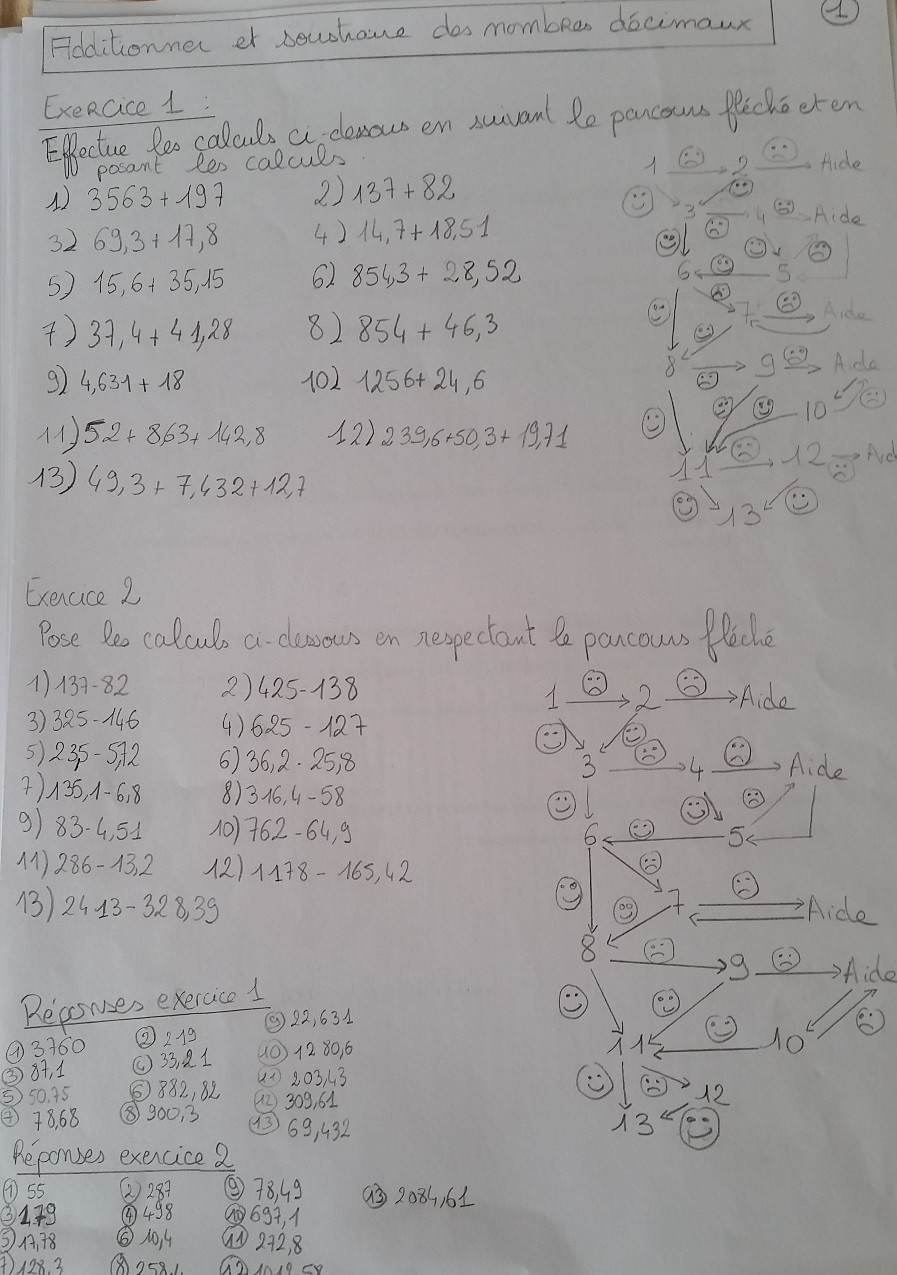
\includegraphics[scale=0.4]{img/parcours_decimaux.jpg}
	\caption{Parcours triangle}
\end{figure}
\paragraph{}Une fois les exercices traités, les élèves pouvaient passer à des problèmes graduellement plus difficiles avec la correction à disposition. Pour ces exercices, j'ai demandé aux élèves de travailler la rédaction et la présentation.

\paragraph{Bilan de l'expérimentation\\}
Dans l'ensemble, j'ai été agréablement surprise par l'esprit de travail et d'entraide qui a régné durant les séances liées à cette séquence. La séance aurait pu se dérouler de manière fluide si je n'avais cependant pas eu de problème avec des élèves très demandeurs d'attention qui refusent de travailler si on n'est pas à côté d'eux. Ces quatre élèves ont gêné l'ensemble de la classe et l'un d'entre eux a même refusé tout travail et a dû être sanctionné.\\
Le reste de la classe a terminé l'exercice et a su, avec mon aide, faire un bilan des techniques de calcul posé. J'ai remarqué moins d'erreurs de calcul par la suite lors de résolution de problèmes mais ne saurais dire si cela est dû au travail en autonomie ou au contenu même de la séquence.\\
Avec du recul, je pense que j'aurais dû rendre la prise en note du bilan obligatoire pour tous les élèves. Ceux-ci ont cependant avancé de manière hétérogène, ce qui a posé problème sur où écrire ce bilan. J'en ai retenu qu'on pouvait prévoir un espace bilan sur la feuille d'exercices, afin qu'elle soit au même endroit pour tous, et facile à retrouver. Après les parcours, les élèves devaient résoudre une série de problèmes et j'ai eu d'avantage de participation lors de la correction, avec beaucoup d'élèves demandant à exposer leur méthode de résolution.
\paragraph{}Les élèves les plus à l'aise et ne souhaitant pas aider un camarade ont cependant fini par épuiser le travail supplémentaire que j'avais prévu, ils ont donc commencé la suite de la séquence et ont même eu l'autorisation de travailler une autre matière pour l'une d'entre eux. Cela me pose la question du travail à demander à ces élèves à l'issue du parcours. J'envisage de leur demander de réaliser une carte mentale autour de la séquence et de ce qu'ils ont compris et employé lors de la séance. Nous avons d'autant plus expérimenté le jeu "Math's up" en demi-groupe\footnote{Jeu où deux équipes s'affrontent : les élèves font deviner une liste de notions mathématiques à leur équipe en les décrivant puis en dessinant lors d'une seconde manche. Pour plus d'information, voir le mémoire d'Alix Duval et d'Antonin Gelamur qui traite en détail de cette activité\cite{maths_up}}, les élèves ont apprécié l'aspect jeu et j'ai observé une amélioration du réemploi des notions par la suite en classe. Les élèves les plus avancés pourraient donc travailler sur quelles notions réemployer pour le jeu par exemple (et de partir de ces notions pour construire une carte mentale en bilan de la séance).

\subsubsection{Troisième parcours différencié (non expérimenté)}
À partir des bilans autour des deux premières séances et suite à des échanges avec Xavière, Victoire, Nadine Grapin et Marine Doceul (tutrice terrain), j'ai rapidement compris qu'il me manquait trois points importants dans mes parcours différenciés :
\begin{itemize}
	\item une évaluation diagnostique sur la notion (cycle 3) ou sur les prérequis de la séquence ;
	\item des balises claires dans le parcours et pour les élèves sur les instants où le travail doit être présenté au professeur, où il faut demander de l'aide ou lorsqu'il faut attendre une mise en commun ;
	\item un ou des moyens d'évaluer l'impact des travaux sur l'acquisition des compétences et des connaissances des élèves, dont le travail en autonomie.
\end{itemize}
\paragraph{} Pour la dernière expérimentation décrite dans le cadre du mémoire, j'ai donc choisi d'évaluer les élèves de sixième sur la séquence \textit{Quadrilatères et triangles particuliers}. L'évaluation diagnostique et son analyse se trouvent en annexe \ref{Eval_diag_ju}. J'ai profité de devoir rendre l'analyse d'une évaluation pour le portfolio pour présenter cette évaluation diagnostique.\\
Suite à cette évaluation, j'ai pu mettre en avant différents types de connaissances sur lesquelles j'ai observé des erreurs :
\begin{itemize}
	\item Connaître les propriétés du carré, rectangle ou losange (hors diagonales)
	\item Connaître les propriétés des diagonales du carré, rectangle ou losange
	\item Connaître les propriétés du triangle rectangle
	\item Connaître les propriétés du triangle isocèle ou équilatéral
	\item Comprendre la notion d'angle
	\item Comprendre la notion de diagonale
\end{itemize}
Certains élèves ont fait des erreurs sur plusieurs catégories de connaissances ; un certain nombre d'élèves n'ont pas répondu à l'évaluation. Un extrait de copies se trouve en annexe \ref{fig:Eval_diag_copies}.\\
Après analyse des difficultés de chacun, j'ai mis en place deux parcours :
\begin{itemize}
\item Quadrilatères
\item Triangles
\end{itemize}
Un exemple de parcours se trouve en annexe\ref{parcours_diff3}. Les élèves devront traiter certaines catégories d'exercices en priorité.
Les élèves à l'aise partout devront tout de même se soumettre aux exercices de chaque catégorie ne serait-ce que pour réinvestir leurs connaissances, voire aider leurs camarades (compétence \textit{travailler en groupe} du référentiel commun de compétences).\\
Une fois qu'ils ont terminé une série d'exercices, par exemple sur les triangles rectangles, si je les considère suffisamment en avance, ils pourront mettre leur nom au tableau dans la colonne \textit{Tuteur triangle rectangle}. De même, les élèves dans le besoin pourront mettre leur nom dans la colonne \textit{À aider triangle rectangle} par exemple.\\
J'ai modifié le plan de table de la classe pour rapprocher des élèves au profil « tuteur » et « demandeur d'aide » et en mettant les élèves en grande difficulté ensemble sur un îlot pour mieux les accompagner.
Les élèves seront munis de leur Ordival et auront chargé un dossier depuis un serveur avant la séance pour disposer de toutes les ressources dont ils pourraient avoir besoin (capsules vidéos, exercices GeoGebra, images \ldots).
Cette expérimentation demande un travail d'organisation important, je compte expérimenter en demi-groupe dans un premier temps, puis en classe entière.\\
J'anticipe une grande difficulté autour de la mise en commun des notions travaillées car plusieurs parcours sont effectués en même temps. Je prévois de mettre des échéances pour chaque parcours et de faire un bilan à mi-parcours et un bilan final. Mon inexpérience sur le traitement de ce chapitre en classe m'empêche de fixer plus de balises. Je profiterai cependant du temps en demi-groupe pour éventuellement traiter des points en plénière.\\
De plus, j'annoncerai en début de séance quels parcours seront priorisés pour les explications individuelles de ma part.

\subsubsection{Bilan évaluation des dispositifs}\label{retour_parcours}
 \remark{Je n'ai pas eu le temps de rédiger cette partie. Les éléments sont repris dans la partie commune}
evaluation travailler en autonomie sur pronote, 2h
questionnaire
retour évaluation
Pour les parcours différenciés, alors que les élèves les plus fragiles demandent un ajustement de certains parcours sur la forme, les élèves ont traité en moyenne deux fois plus d'exercices lors des séances en autonomie sur les séquences numériques. Les exercices de géométrie ont quant à eux été traités de manière plus difficile selon les compétences testées. De manière générale, les élèves ont traités plus d'exercices qu'à l'accoutumée, mais j'ai dû intervenir de manière plus fréquente, avec beaucoup d'interventions en plénière


\subsection{Tutorat entre élèves (Victoire)}
\subsubsection{Motivations}
Le tutorat entre élèves peut être une autre source d'apprentissage : pendant que
l'un enseigne, l'autre apprend.

L'enseignement en lui-même est une forme d'apprentissage : la personne qui
enseigne doit assez bien maitriser la notion, les méthodes et le vocabulaire
utilisé afin de pouvoir l'enseigner à quelqu'un d'autre. Savoir enseigner
demande plus que simplement maitriser une technique ; cela demande de savoir
pourquoi on peut utiliser une technique, et quel raisonnement se trouve derrière
la technique.

Permettre et encourager les élèves à enseigner serait donc une autre méthode de
faire apprendre une notion à un élève. C'est aussi une opportunité pour un élève
qui n'aurait pas compris d'avoir un autre regard sur une notion, et un cours
individualisé. C'est le raisonnement derrière la « méthode Feynman », une méthode
qui applique la méthode d'enseignement de Richard Feynman.\footnote{\url{https://www.youtube.com/watch?v=_f-qkGJBPts} vidéo présentant la méthode Feynman.}

%Est-ce qu'un élève est plus réceptif a un cours individualisé ?
% Demander un retour de Xavière sur la chose
% Voir la réceptivité des élèves a un cours en vidéo

\subsubsection{Risques et contraintes}

Tout comme on n'imaginerait pas un enseignant ne pas maitriser son domaine, il
faudra s'assurer que l'élève maitrise le sien avant de l'enseigner à un autre
élève.

Il y a également un risque de créer ou d'aggraver une scission dans la classe :
les tuteurs pourraient être vus comme des élèves étant privilégiés, et ainsi créer
une hiérarchie dans la classe.\cite{pedagogie_cooperative_hierarchie}

Il faut également bien maitriser le minutage de sa séance afin de pouvoir controler
les déplacements d'élèves dans la salle de classe : trop de déplacements causent
trop de bruit, et deviennent donc nuisibles à tous.

\subsubsection{Expérimentations}

\paragraph{Mise en autonomie sans préparation}

Une des méthodes de mise en autonomie qui parait le plus simple d'accès est de
simplement les laisser faire et d'autoriser les élèves à s'entraider. J'ai
considéré cette possibilité pour plusieurs raisons :
\begin{itemize}
    \item elle ne demande pas de préparation particulière préalable ;
    \item les règles sont simples pour les élèves ;
    \item elle permet l'apprentissage entre élèves (voir les bénéfices au paragraphe précédent) ;
    \item personne ne m'a dit de ne pas faire ça.
\end{itemize}

Les objectifs de cette expérimentation étaient :
\begin{enumerate}
    \item permettre aux élèves avancés de ne pas « rien faire » ;
    \item permettre aux élèves ayant des difficultés d'avoir une aide plus
    rapidement ;
    \item augmenter l'expertise des élèves avancés, les forçant à adopter d'autres
    façons de voir la notion ;
    \item réduire le nombres d'appels au professeur, restant ainsi disponible
    pour les questions avancées ;
    \item réguler le niveau de bruit\footnote{Ne pas confondre bruit et niveau sonore} de la classe.
\end{enumerate}

Lors d'une séance d'exercices, j'ai donc autorisé les élèves qui voulaient
aider leurs camarades à se lever. Les premiers élèves demandaient à se lever, et
avaient bel et bien fini correctement leurs exercices. Au fur et à mesure, des
élèves avaient pris la liberté de se lever, sans avoir forcément fini leurs exercices,
et sans forcément avoir correctement répondu. Et je ne suis pas persuadée que
tous les élèves s'entraidaient effectivement.

Je considère que cette première expérimentation s'est donc soldée par un échec, car
l'objectif de réguler le niveau de la classe n'était pas atteint : certes certains
élèves sérieux aidaient d'autres élèves qui en avaient besoin, mais d'autres tiraient
profit de la situation pour bavarder, et ainsi perturber d'autres élèves qui
auraient pu réussir les exercices dans des conditions normales.

Pire encore : certains élèves de bonne foi, avaient fini leurs exercices et aidaient
leurs camarades, mais leurs réponses et méthodes étaient fausses, et propagaient
ainsi de mauvaises méthodes au reste de la classe !

En conclusion, cette méthode ne fonctionne pas (pas de réduction, voire augmentation
du bruit en classe), et est même contre-productive car elle nuit au développement
de certains élèves.

\paragraph{Tétra-aide}

Le concept du tétra-aide est simple : un tétraèdre permet à l'élève d'indiquer
son besoin d'aide en fonction du sommet orienté vers le haut :
\begin{enumerate}
    \item Tout va bien
    \item J'ai une question non-urgente
    \item À l'aide !
    \item J'aide ou je suis aidé par quelqu'un
\end{enumerate}

Utiliser le tétra-aide permet d'avoir une meilleure visualisation de ceux qui ont
besoin d'aide, et de faire un meilleur triage parmi ceux qui ont besoin d'aide :
ceux qui bloquent vraiment sur l'exercice et ont une question technique, et ceux
qui ont fini ou ont une question qui n'a pas directement rapport au cours.

Lent à démarrer

Attention, les élèves détruisent leurs tétra-aides

À faire en plus gros parce qu'ils ont tendence à ne pas se voir

\subsubsection{Pistes de réflexion}

\subsubsection{Aménagement de l'espace classe}

L'aménagement de l'espace classe peut permettre une meilleure collaboration entre
élèves. La disposition classique (en « autobus » ou « rangs d'ognon ») ne permet
qu'une interaction possible : entre le professeur et les élèves.

D'autres dispositions permettent une meilleure collaboration entre élèves : par
exemple, en îlots bonifiés\cite{ilots_bonifies}, ou en U\cite{amenagement_classe}.

\subsection{Évaluations différenciées (Victoire)}
\subsubsection{Motivations}

L'idée de différencier les évaluations m'est venue au contact de Julia et Xavière,
qui évaluent toutes les deux par compétences. Mon collège est encore resté aux
notes, et je voulais faire en sorte de pouvoir évaluer mes élèves sur des
compétences, et donc leur proposer plusieurs manières de prouver leur maitrise
d'une compétence. Différencier les évaluations est donc un choix naturel.

\subsubsection{Comment je l'ai découvert}
Avec Sandrine, nous étions toutes les deux
intéressées par les évaluations différenciées. Au départ, nous voulions tester
ceci sous sa forme la plus simple : pour un exercice, les élèves pourraient
choisir une version simple, qui rapporterait $n$ points, ou\footnote{Ici, un ou
exclusif} une version plus experte, qui rapporterait $m$ points\footnote{$n < m$}.

Alors que nous allions passer à la rédaction de nos sujets, Julia me fournit
un article traitant des évaluations différenciées\cite{differenciation_devoir_surveille}.
En lisant cet article, je me rends compte que la manière dont Sandrine et moi
allions justement procéder d'une manière qui n'est pas recommandée par les
auteurs\footnote{Cette fois-ci, il y a vraiment quelqu'un pour nous dire de ne
\textbf{pas} faire ce que nous avions prévu.} !

\subsubsection{Expérimentation}

Les auteurs recommandent, plutôt que de proposer aux élèves le choix entre 2
versions d'un exercice, de proposer un « buffet d'exercices » : par exemple, proposer
12 exercices à 2 points chacun\footnote{Les valeurs en points de chaque exercice
peut varier bien sûr}, et laisser aux élèves choisir quels exercices ils veulent
effectuer. Dans cet exemple, il est possible d'obtenir jusqu'à 24 points, et
donc la note de 24/20 !

J'ai donc rédigé un sujet (voir annexe \ref{sujet_differencie}), avec les objectifs suivants
en tête :

\begin{itemize}
    \item permettre aux élèves de prouver leur maitrise d'une notion par différentes manières ;
    \item faire en sorte qu'un élève \textbf{doive} au moins faire un exercice qui évalue une notion donnée pour chaque notion ;
    \item donner du challenge aux élèves en avance ;
    \item redonner confiance aux élèves en difficulté mais qui travaillent.
\end{itemize}

Au final, lors et après l'évaluation, j'ai pu remarquer les choses suivantes :
\begin{itemize}
    \item il y a peu d'effets sur les élèves non-travailleurs et ceux qui sont
    en avance. Par contre, il y a eu une petite amélirotation chez les élèves
    « entre-deux », mais travailleurs ;
    \item l'évaluation était trop difficile, d'où une difficulté d'observer une
    amélioration chez la population ciblée ;
    \item tous les élèves ont travaillé jusqu'au bout.
\end{itemize}

Après l'évaluation, les exercices de base ont été corrigés, et un corrigé complet
a été mis à disposition sur le cartable en ligne.

Le point essenciel à corriger dans mon expérimentation est le sujet de l'évaluation :
j'ai énormément de mal à rédiger des sujets d'évaluation longs\footnote{
Notamment parce que ça prend énormément de temps à préparer, encore plus à corriger,
et que ça demandait une énergie que je n'avais pas cette année.
}.

\subsubsection{Pistes de réflexion}

Pour de prochaines évaluations différenciées, voici ce que je changerai :
\begin{itemize}
    \item rédiger des sujets moins longs, sur moins de notions ;
    \item essayer d'appliquer ce système à des interrogations courtes de début d'heure ;
    \item voir si, dans un prochain établissement, ce système est requis si l'établissement
    utilise une évaluation par compétences.
\end{itemize}

Il faudrait également que je me renseigne sur le principe des ceintures de compétences,
qui donnent un peu plus de liberté dans le rythme d'apprentissage des élèves.

\subsection{Différenciation par les supports (Xavière)}

% BILAN D'ETAPE

%Au départ, je suivais plusieurs pistes de différenciation. En particulier, je souhaitais instaurer un parcours différencié pour mes deux classes principales, selon le modèle présenté par Julia. Ma tutrice ESPÉ m’a fortement conseillé de me limiter à ma classe de 4e, plus difficile à mettre au travail.
%
%J’ai également créé une évaluation à jokers avec ma classe de 4e. Les jokers sont des petits papiers contenant une indication sur l’exercice que je distribue aux élèves en échange d’une pénalité minime sur la note. Cette évaluation a obtenu un franc succès.
%J’ai également commencé le travail d’auto-évaluation avec mes 5e. Ce qu’il manque pour approfondir ce point, c’est créer une métrique adaptée. Pour le moment je n’ai pas de retour quantifiable.
%
%Sur les conseils de Nadine Grapin, je me suis concentrée sur un axe de recherche en particulier, et j’ai choisi l’auto-évaluation. Pour cela, je souhaite m’intéresser aux supports.
%
%Mes classes sont caractérisées par la présence de mauvais lecteurs (des élèves en très grande difficulté en Français, sans toutefois présenter des troubles dys). Il est donc primordial de m’assurer que :
%\begin{enumerate}
%    \item ils se construisent des images mentales correctes et cela ne peut pas toujours passer par une compréhension de la trace écrite. J’ai remarqué, en particulier pour la classe de 5e, que les images mentales dynamiques (nécessitant des manipulations) étaient plus facilement assimilées et restituées par les élèves.
%    \item les consignes données à l’oral sont parfaitement comprises de tous
%\end{enumerate}
%
%De plus, comme je vise l’autonomie des élèves à la fois en classe et hors classe, je dois compléter cette approche par d’autres supports, en particulier des fiches de correction. Pour le moment, je les guide sur la construction de fiches de révision agréables à l’oeil pour que les élèves s’y réfèrent plus volontiers. Je souhaite me tourner progressivement vers des fiches de correction, puis d’auto-correction, avec un guide de construction de fiches créé par les élèves. L’objectif final est de produire des grilles d’auto-évaluation.
%Tout ceci est très expérimental et je ne suis pas encore en capacité de mesurer quantitativement les conséquences de la multiplication des supports

%{\color{red}Tous les passages écrits en rouge dans cette partie sont des remarques destinées à améliorer le contenu, souvent sur la forme, ou sont des réflexions ou des questionnements.}
%
%\subsubsection{Motivations}
%
%{\color{red}Rappels en vrac de ma ligne directrice pour mes expérimentations. À reformuler et à remettre en contexte. Ce sont les conseils donnés par ma tutrice en début d'année que j'ai essayé d'appliquer de mon mieux, à l'exception des vidéos.}
%
%\begin{itemize}
%\item Se renseigner sur la différenciation en axant sur les images mentales ;
%\item diversifier les images mentales (toutes ne fonctionnent pas sur tous les élèves) ;
%\item diversifier les images mentales grâce aux supports :
%\begin{itemize}
%\item cartes mentales (en particulier celles centralisant toutes les façons de répondre à un problème donné, par exemple comment montrer que deux droites sont parallèles) ;
%\item manipulations manuelles/gestuelles ;
%\item utilisation de geogebra par les élèves (et non par moi) ;
%\item vidéos explicatives ;
%\item fiches de méthodologie cartonnées, idéalement faites spontanément par les élèves ;
%\end{itemize}
%\item le but est de fixer par écrit les images mentales.
%\end{itemize}
%
%\paragraph{Quelques détails}
%
%Le but est que \textbf{les élèves créent eux-mêmes leurs outils}. La priorité est aux fiches méthodes, fiches erreur et cartes mentales. Sur les fiches méthodes, lorsque nous voyons une méthode technique en cours, les élèves en font une fiche cartonnée qui leur servira de référence lors des exercices et évaluations. La fiche erreur est construite par l'enseignant sur la base de plusieurs publications des élèves. Je leur donne un bilan récapitulatif des erreurs à éviter. Eux en font une fiche qui complète la fiche méthode. Pour la carte mentale, il est convenu avec ma tutrice que je leur fournisse une base qu'ils complètent.
%
%Je peux aussi leur fournir une carte mentale de résumé de cours, mais comme cela consiste essentiellement en de la recopie du cours, \textbf{ne pas la considérer comme un exercice mathématique} à part entière et ne pas leur donner à compléter.
%
%{\color{red}Faire de tout ce paragraphe un tableau synthétique.}
%
%Le but est de leur permettre de s'emparer, de s'approprier les notions vues en classe et de leur constituer {\color{red}(ou apprendre à constituer)} une banque de ressources qu'ils utiliseront en classe sur exercices ou à la maison pour s'auto-corriger.
%
%Ce travail sera essentiellement \textbf{étudié sur ma classe de 5\up{e}}, mais ceci est proposé sur les deux classes.
%
%Note : ma tutrice ESPÉ m'a conseillé de me limiter aux parcours différenciés aux 4\up{e}. Ceci étant couvert par Julia, je n'en parlerai pas. {\color{red}Retour très intéressant de Claire sur le problème du saucissonnage sur la séquence Pythagore, cela vaut sans doute la peine d'en parler en discussion.}\\
%
%{\color{red} Pour ce qui suit, j'ai le sentiment que cela fait beaucoup trop. J'ai entamé un très gros travail sur la symétrie et j'ai également des scans de copies d'élèves appuyant la nécessité de corriger une mauvaise conception pour les angles alternes-internes. La partie sur le calcul algébrique est sans doute dispensable si je n'en ai pas le temps et je manque de productions d'élèves pour l'étayer. Enfin, la dernière partie sera uniquement axée sur le traitement des erreurs à éviter (ou dans le cas présent, des éléments manquants). J'ai à la fois les productions d'élèves scannées, le fichier regroupant les productions les plus intéressantes et la fiche méthodologique construite par les élèves. Les cartes mentales ont surtout été vues avec les 4e, sur le principe elles reprennent ce qu'on a fait avec les fiches méthodologiques. J'ai encore une séquence à finir et une autre à faire avec mes 5e avant de pouvoir faire des cartes mentales intéressantes portant sur plusieurs séquences.}

%\subsubsection{Symétries : manipulations manuelles et sur geogebra - fiches de méthodologie}
%
%Le but est de montrer comment j'ai ajouté des couches successives pour renforcer les deux images mentales principales en symétrie axiale et symétrie centrale. J'ai toujours un problème avec mon élève italien qui a tendance à effectuer des translations.
%
%\paragraph{Les cocottes en symétrie}
%
%\paragraph{Remplacement progressif par les mains}
%
%\paragraph{Utilisation de Geogebra en auto-correction}
%
%Lien vers ma séance TICE. Probablement pas aussi développé que le reste.
%
%\paragraph{Fiches de méthodologie}
%
%\paragraph{Retours, productions d'élèves}
%
%Lien vers mon analyse d'évaluation + la toute dernière évaluation faite. Parler de mon élève italien ?
%
%\subsubsection{Angles alternes-internes : comment corriger une potentielle image fausse}
%
%\paragraph{Situation qui a amené les élèves à créer cette image mentale fausse}
%
%Lien vers mini-évaluation + stats rapides sur présence de l'erreur dans les copies.
%
%\paragraph{Utilisation de Geogebra pour corriger une potentielle image mentale fausse}
%
%\paragraph{Une autre approche : la libellule et la coccinelle}
%
%Très rapide, l'évaluation récente montre que cette image mentale n'est pas très populaire au sein de ma classe, alors qu'elle est très utilisée dans les deux autres classes de 5\up{e} (le timing où elle a été présentée est différent).
%
%\paragraph{Initiation à la démonstration : erreurs et correction par les pairs}
%
%{\color{red} Je ne sais pas si celui-ci a sa place dans ce mémoire, dans la mesure où cela se passe intégralement à l'oral}
%
%\paragraph{Cartes mentales - droites parallèles / calcul d'angles}
%
%Les deux sont envisageables et liées à cette séquence. {\color{red}Je ne sais pas si j'aurai le temps de les amorcer avant la date de rendu du mémoire.}
%
%\subsubsection{Calcul algébrique : deux approches différentes pour toucher un maximum d'élèves}
%
%\paragraph{Nombres relatifs - approche vectorielle}
%
%\paragraph{Nécessité de recourir à une deuxième approche}
%
%\paragraph{Nombres relatifs - approche [nom à définir plus tard]}
%
%\subsubsection{Gestion de données : trouver les erreurs à éviter}
%
%\paragraph{Problème initial et productions d'élèves}
%
%\paragraph{Fiche méthodologique résultante}
%
%\subsubsection{Retours élèves}

\subsubsection{Motivations}

Le but de mon expérimentation était d'amener les élèves de ma classe de 5\up{e} à un niveau suffisant d'autonomie pour créer eux-mêmes leurs propres outils de travail (voir \textsc{Figure \ref{org:xav}} ci-dessous). Pour atteindre ce but, j'ai exploré plusieurs pistes et je souhaite en aborder deux en particulier : le travail effectué autour de la symétrie dans un premier temps et le travail effectué sur les angles alternes-internes dans un deuxième temps.

\begin{figure}[h!]
    \centering
    \tikzstyle{cat1} = [rectangle, rounded corners, minimum width=3cm, minimum height=1cm, text centered, text width=3cm, draw=black, fill=black!0]
\tikzstyle{cat2} = [rectangle, minimum width=3cm, minimum height=1cm, text centered, text width=3cm, draw=black,  fill=black!10]
\tikzstyle{cat3} = [rectangle, minimum width=5cm, text centered, text width=5cm, minimum height=1cm, draw=black,  fill=black!10]

\tikzstyle{arrow} = [thick,->,>=stealth]

\begin{tikzpicture}[node distance=3cm]
\node (auto) [cat2] {Développer l'autonomie};
\node (img) [cat2, right of=auto, xshift=7cm] {Images mentales correctes};
\node (pb) [cat3, below of=auto, xshift=5cm] {Élèves assez autonomes pour construire par eux-mêmes les outils pour s'approprier une notion};
\node (outils) [cat2, below of=pb] {Outils};
\draw [arrow] (auto) |- (pb);
\draw [arrow] (img) |- (pb);
\draw [arrow] (pb) -- (outils);
\node (fiche1) [cat1, left of=outils, xshift=-2cm] {Fiches erreur};
\node (fiche2) [cat1, below of=outils, xshift=-5cm, yshift=1cm] {Fiches méthodologiques};
\node (carte1) [cat1, below of=outils, yshift=1cm] {Cartes mentales bilan};
\node (geogebra) [cat1, right of=outils, xshift=2cm] {GeoGebra et tableur};
\node (carte2) [cat1, below of=outils, xshift=5cm, yshift=1cm] {Cartes mentales transversales};
\draw [arrow] (outils) -- (fiche1);
\draw [arrow] (outils) -- (fiche2);
\draw [arrow] (outils) -- (geogebra);
\draw [arrow] (outils) -- (carte1);
\draw [arrow] (outils) -- (carte2);
\end{tikzpicture}

    \caption{Organigramme des ressources nécessaires pour amener des élèves à créer leurs propres outils en toute autonomie}
    \label{org:xav}
\end{figure}

\paragraph{Présentation succincte des outils que les élèves sont amenés à utiliser sur l'année}

\remark{Ajouter une phrase d'introduction ici}
\begin{itemize}
	\item [Les fiches méthodologiques :] accompagnement de cours, elles se présentent sous la forme d'une méthode écrite sur une fiche cartonnée et illustrée selon les goûts des élèves. Les élèves les utilisent lorsqu'ils travaillent sur des exercices ou lors des devoirs avec ma permission.
	\item [Les fiches erreur :] ces fiches viennent en complément des fiches méthodologiques. Elles sont utilisées pour aider les élèves à valider ou invalider un résultat. C'est un axe de recherche que je n'ai pas assez développé cette année. J'ai limité mes expérimentations à la présentation d'extraits de copies à mes élèves pour générer des débats. Il en a résulté des fiches méthodologiques au lieu de fiches erreur.
	\item [Les cartes mentales :] initialement, si l'on se réfère à la  \textsc{Figure \ref{org:xav}}, il était prévu que je travaille sur deux types de cartes mentales avec les élèves. Le premier type est une carte rappelant les notions importantes du cours, telles qu'on les trouve dans les leçons de cycle 3 ou les manuels de cycle 4. Elle sert de bilan et est surtout utilisée lors des révisions. Les élèves en ont réalisé quelques-unes tout au long de l'année, toujours d'après un modèle établi en commun en classe. \\
	Le second type est une carte mentale transversale, répondant à une question\footnote{Par exemple : "Comment prouver que deux droites sont parallèles ?"} qui peut être traitée à l'aide de procédures issues de plusieurs séquences. J'ai manqué de temps et de recul sur le programme pour mettre ce type de carte mentale en place.
	\item [L'utilisation des TICE] (Technologies de l'Information et de la Communication pour l'Enseignement) : les élèves manipulent régulièrement en cours d'année les logiciels utilisés en mathématiques (Geogebra et les tableurs) pour apprendre à valider un résultat ou une conjecture de manière autonome.
\end{itemize}

\subsubsection{Pourquoi la différenciation est importante pour l'autonomie des élèves}

Lorsqu'on cherche à rendre ses élèves autonomes, on se rend vite compte que la différenciation intervient à plusieurs niveaux. Si l'on se réfère à l'organigramme présenté en \textsc{Figure \ref{org:xav}}, la première entrée est la poursuite du développement de l'autonomie, entrepris au cycle 3. J'ai suivi deux axes :
\begin{itemize}
    \item faire acquérir aux élèves le réflexe d'utiliser leurs outils (relire une fiche méthodologique quand on bloque devant un exercice, se référer à la fiche-erreur pour valider un résultat, utiliser les cartes mentales pour réviser...) ;
    \item développer le travail en autonomie en classe, l'objectif au troisième trimestre étant de m'assurer que mes élèves sont en activité un tiers du temps.
\end{itemize}
Concernant le premier point, la différenciation passe essentiellement par une attention particulière aux consignes données et le choix des procédures de résolution (différenciation simultanée \cite{Eduscol}). Ce point ne sera pas détaillé ici.

Concernant le second point, Il faut distinguer deux moments forts du cours lorsqu'on travaille sur les images mentales avec les élèves. Pour rappel, une image mentale est "une représentation d'une information sensitive sans perception d'un stimulus externe" \cite{mimagery}. Cette représentation peut être mémorisée ou imaginée. En mathématiques, les images mentales servent à donner du sens à un concept non perceptible par nos sens.

Dans un premier temps, j'établis avec mes élèves une image mentale (ou plusieurs) à laquelle se référer lorsqu'ils rencontrent un nouveau concept. La différenciation porte sur la variété des supports présentés aux élèves (différenciation successive \cite{Eduscol}).

Dans un deuxième temps, après avoir observé les élèves travailler sur le nouveau concept avec leur(s) image(s) mentales, j'entre parfois dans une phase de remédiation, l'image mentale présentée initialement étant mal assimilée ou incomplète. La remédiation passe soit par la présentation d'une autre image mentale, soit par un changement de support pour une même image mentale.

Le travail présenté dans ce mémoire porte sur ces deux temps de fabrication d'une image mentale correcte :
\begin{itemize}
    \item une première sous-partie est consacrée à variété des supports utilisés pour passer d'une perception de la symétrie (axiale et centrale) à une image mentale en variant les sens utilisés ;
    \item une seconde sous-partie est consacrée à la remédiation d'une mauvaise conception des angles alternes-internes.
\end{itemize}

La différenciation intervient également au niveau des outils eux-mêmes : les logiciels nécessitent une phase de prise en main et un de mes axes cette année a été de proposer des exercices différenciés sur support informatique, adaptés à l'aisance des utilisateurs avec les logiciels. J'en parle très brièvement au moment où j'aborde la section consacrée aux symétries.

\subsubsection{Différencier pour acquérir une image mentale : la symétrie}

%Le but est de montrer comment j'ai ajouté des couches successives pour renforcer les deux images mentales principales en symétrie axiale et symétrie centrale. J'ai toujours un problème avec mon élève italien qui a tendance à effectuer des translations.

J'ai commencé à construire la séquence dédiée à la symétrie axiale à l'aide du livre \textit{Des maths ensemble et pour chacun 5\up{e}} \cite{mepcc} (séquence 2, pages 88-103). La première activité présentée utilise des silhouettes de cocottes et les indications à destination de l'enseignant emploient également les cocottes (voir \textsc{Figure \ref{fig:cocottes}} et annexe \ref{annexe:symetrie-act}). J'ai repris cette idée pour mon expérimentation.

\begin{figure}[h!]
    \centering
    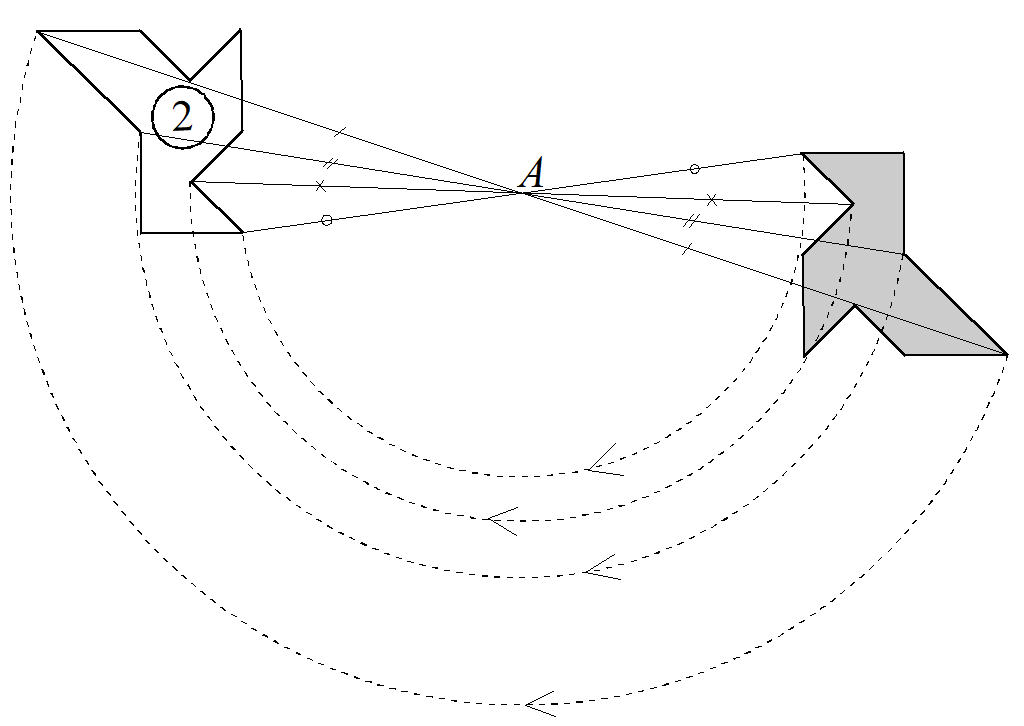
\includegraphics[width=0.6\linewidth]{img/cocottesmepcc.png}
    \caption{Figure accompagnant les explications destinées à l'enseignant et pouvant être photocopiées et distribuées aux élèves}
    \label{fig:cocottes}
\end{figure}

\paragraph{Création d'un outil à manipuler : les cocottes}

En premier lieu, avant de leur donner l'activité du livre qui consistait à classer des couples de cocottes grises et blanches par type de transformation (symétrie axiale, symétrie centrale et translation), j'ai appris aux élèves à créer deux cocottes identiques, excepté un signe distinctif, avec une feuille de papier. Lorsqu'ils ont démarré l'activité, ils superposaient la cocotte blanche sur la cocotte grise et essayaient de trouver quelle manipulation ils faisaient avec les mains pour arriver au résultat présenté sur la feuille d'activité.

Très vite, les élèves ont retrouvé l'image du miroir pour la symétrie axiale et le mouvement rectiligne pour la translation. Ils ont également découvert que leurs cocottes effectuaient un arc de cercle pour la symétrie centrale.

Les cocottes sont pratiques pour deux raisons : premièrement, elles représentent concrètement les figures de l'énoncé. Les élèves n'ont pas à faire un effort d'abstraction supplémentaire pour passer de la manipulation à la situation de l'énoncé. Deuxièmement, elles se glissent toutes dans une pochette et sont facilement transportables. Même si elles sont égarées, elles sont très rapides à fabriquer.

\paragraph{Remplacement progressif par les mains}

La phase de consolidation de l'image mentale s'est faite en deux temps. Tout d'abord, j'ai présenté aux élèves des exercices où les figures n'étaient plus des cocottes, pour qu'elles prennent le statut d'outil. Puis certains élèves ont compris qu'ils effectuaient les mouvements avec les mains qui tenaient les cocottes et ont commencé à faire les manipulations avec les mains seulement.

À ce moment, j'ai moi-même commencé à évoquer les images mentales du miroir et de la rotation avec mes mains sans tenir les cocottes. Le comportement s'est généralisé à l'ensemble de la classe.

\paragraph{Fiches méthodologiques}

Lors du travail sur cette séquence, les élèves ont construits deux fiches méthodologiques pour la symétrie axiale et deux fiches méthodologiques pour la symétrie axiale.

La première fiche détaille la construction de l'axe de symétrie ou du centre de symétrie. Elle a été construite en commun avec la classe après leur avoir fait construire les axes de symétrie et les centres de symétrie à nouveau sur la première activité de la séquence. La fiche résulte du débat généré à la fin de l'exercice et synthétisé par un élève. À ce moment de l'expérimentation, les élèves notaient sur leur feuille des flèches de rotations comme celles que l'on voit sur la \textsc{Figure \ref{fig:cocottes}} pour évoquer l'image mentale qu'ils s'étaient construite.

La seconde fiche détaille la construction du symétrique d'une figure par symétrie axiale ou centrale.

Des exemples sont disponibles dans l'annexe \ref{annexe:symetrie-fiches}.

Ces fiches ont été reproduites sur papier cartonné et étaient utilisées lors des exercices d'entrainement sur la durée ou lors de certains devoirs surveillés.

\paragraph{Utilisation de GeoGebra}

J'ai beaucoup travaillé cette séquence sur la durée et je me suis rendue compte en cours d'année que certains élèves oubliaient l'image mentale s'ils ne travaillaient pas assez régulièrement dessus. Pour les aider, sur un conseil de ma tutrice terrain, madame Hizembert, j'ai créé une séance en salle informatique pour leur apprendre à utiliser de façon autonome GeoGebra pour s'entrainer chez eux.

Un résumé de la séance est présent dans l'annexe \ref{annexe:symetrie-tice}

Avec le recul que j'ai à présent et suite à des discussions avec Madame Hizembert, j'aurais pu utiliser davantage GeoGebra pour renforcer les images mentales des élèves. La séance informatique est intervenue trop tard dans l'année. J'ai également découvert que le manuel \textit{Des maths ensemble et pour chacun 5\up{e}} s'accompagnait d'un site\footnote{Site compagnon : http://edition.crdp-nantes.fr/?id=maths-ensemble-et-pour-chacun} permettant de télécharger des ressources qui permettent de visualiser l'image mentale de la rotation avec GeoGebra.

\subsubsection{Remédier à une mauvaise conception : les angles alternes-internes}

Lorsque j'ai introduit les angles alternes-internes aux élèves, j'ai très rapidement réutilisé les propriétés de conservation de la symétrie centrale (travail sur la durée), couplée à une conjecture visualisée à l'aide de GeoGebra, alors que la définition d'angles alternes-internes n'avait pas été vue. En conséquence, sur une évaluation diagnostique qui a suivi peu après, j'ai constaté que pour beaucoup d'élèves (voir annexe \ref{annexe:angles-prod1}, deux angles alternes internes étaient \textbf{toujours} définis par deux droites \textbf{parallèles} et une sécante. J'ai aussi pu constater que pour un grand nombre d'élèves, il n'existe qu'une paire d'angles alternes-internes, la paire d'angles aigus ou au contraire la paire d'angles obtus.

J'ai choisi deux axes de remédiation. Tout d'abord, j'ai travaillé sur des exercices très progressifs (sur le principe du parcours différencié). Puis j'ai présenté une nouvelle image mentale aux élèves qui avaient encore du mal à transposer les mots de la définition des angles alternes-internes à une application concrète.

\paragraph{Exercices progressifs}

Les trois fiches d'exercice sont disponibles dans l'annexe \ref{annexe:angles-fiches}

La première fiche d'exercices ne mentionne pas le statut des droites définissant les angles alternes-internes. Le but était de simplement vérifier si la définition correspondaient à ce qu'ils voyaient (présence d'angles alternes-internes, correspondants, alternes-externes, opposés par le sommet et le cas particulier des angles alternes-internes où l'un des angles est un angles droit).

Puis j'ai rétabli que la mention de droites parallèles n'intervient nullement dans la définition mais est prépondérante dans la propriété \textit{"Deux droites parallèles coupées par une droite sécante déterminent des angles alternes-internes de même mesure"} (et sa réciproque). Pour renforcer cette idée, j'ai présenté une nouvelle feuille d'exercices contenant des schémas où toutes les situations montrent des droites parallèles, mais où la mention de droites parallèles est parfois absente (l'un des objectifs étant de travailler sur le passage progressif à la géométrie abstraite).

La troisième feuille d'exercices a été distribuée une fois que les problèmes relevés ont été corrigés et présente des situations de plus en plus complexes.

J'avais dans l'idée d'appliquer le principe des parcours différenciés mais l'exécution a été maladroite. La fiche 3 est celle où le principe apparait le plus clairement : seules les situations A, B et C étaient à traiter, les autres étaient réservées aux élèves plus avancés.

\paragraph{Remédiation par l'acquisition d'une nouvelle image mentale}

Suite à tout ce travail, j'ai constaté que certains élèves avaient encore des difficultés à visualiser les paires d'angles alternes-internes et plus particulièrement le concept derrière le mot alterne. Je leur ai donc conté une histoire venant de ma tutrice terrain, Madame Hizembert : "Deux insectes, une coccinelle et une libellule ont rendez-vous d'un coté du pont au-dessus de la rivière. Problème, elles sont chacune d'un coté différent du pont. Elles ne se rencontreront jamais."

Ce petit texte a été accompagné d'un dessin que quelques élèves se sont appropriés (voir quelques copies d'élèves dans l'annexe \ref{annexe:angles-prod2}). à ma surprise, après avoir présenté cette histoire à toute la classe et après un rapide sondage, il s'est avéré que ceux pour qui la notion était acquise n'appréciaient pas du tout cette histoire.

\subsubsection{Autres expérimentations}

De la même manière que j'ai essayé ..K.

\subsubsection{Retours des élèves}

Cette partie de l'expérimentation n'est pas encore menée. Pour pousser plus loin ...

Il s'agit d'un questionnaire à faire remplir par les élèves, en particulier sur l'utilisation des fiches méthodologiques chez eux, sur l'utilisation de GeoGebra/Excel.

% Parle peut-être plutôt d'un tableur, plutôt qu'Excel. Si on peut éviter de mentionner
% des logiciels privateurs quand des alternatives libres sont disponibles, tant mieux !
% Il y a déjà assez de lobbying de la part des GAFAM dans l'EN…

\section{Discussions}
Dans cette partie, nous faisons le point sur nos pratiques avec un regard critique enrichi par les retours de nos collègues et de nos élèves, et confrontés aux expérimentations d'autres collègues de l'ESPÉ. Nous aborderons également la question de l'impact des pratiques expérimentées sur l'acquisition des connaissances et des compétences de nos élèves, et sur leur capacité à travailler en autonomie. Nous traiterons enfin des autres dispositifs mis en place lors de notre année de stage et dont l'analyse (brève) peut, selon nous, enrichir ce mémoire.
\subsection{Discussion autour de nos pratiques}
Comme indiqué dans la partie \ref{Expérimentations}-Expérimentations, nous avons effectué des choix d'expérimentation différents au regard de nos besoins et de nos lectures de début d'année.\\

\subsubsection{Comparaison de nos expérimentations}
\paragraph*{}Nous avons toutes choisi de mettre en place des dispositifs incluant tous élèves de nos classes. Ces dispositifs ont des impacts plus ou moins importants sur les élèves selon leur niveau, mais nous avons choisi de tous les inclure dans nos dispositifs.\\
Dans les faits, le tutorat des élèves, les exercices de remédiation ou les défis des parcours différenciés vont avoir une incidence plus importante sur les élèves en grande difficulté ou au contraire très à l'aise sur les compétences travaillées. Les évaluations différenciées et les supports adaptés à chaque élève sont en revanche supposées avoir un impact sur l'autonomie et l'acquisition des compétences de tous les élèves, sans distinction de niveau.\\
\remark{Je ne sais pas si ce que j'écris vous paraît pertinent. Je pense que c'est une première différence intéressante entre les dispositifs. Pour la suite, @Xavière, je te laisse modifier à ta guise!}
\paragraph*{}Dans la construction des parcours différenciés, Xavière et Julia ont toutes les deux mis en place des parcours de formes différentes. Alors que Julia propose un guide de parcours ainsi qu'une série d'exercices selon la réussite ou non de l'élève, Xavière propose une feuille d'exercices avec une version plus ou moins difficile de l'exercice (variation dans le choix des variables didactiques) et l'élève choisit celui qu'il traite \remark{il me semble, de mémoire}. Dans les deux cas, un élève en difficulté aura la possibilité de traiter un exercice plus facile pour appréhender une notion, et les élèves les plus à l'aise auront accès à des problèmes plus difficiles à aborder.\\
La différence de présentation présente cependant une différence d'approche très intéressante car dans l'expérimentation de Julia, les élèves n'ont pas le choix de traiter la version facile d'un exercice ou le défi de leur parcours. Ils doivent également identifier par eux-même une situation d'échec ou de fragilité dans le traitement d'un exercice, qui demande d'effectuer un exercice supplémentaire. Au contraire, l'approche de Xavière donne le choix aux élèves dans le niveau de l'exercice à traiter. D'un côté on peut s'attendre à ce que les élèves à l'aise essaient toutes les versions ou que les élèves ne choisissent que la facilité, d'un autre côté, un élève en difficulté ne passera pas par une étape « d'échec » avant de traiter un exercice plus abordable.
\paragraph*{}
\remark{Vous avez toutes les deux testé des évaluations différenciées mais pas du tout sous la même forme (je crois que Xavière c'était plus dans le sens de s'auto évaluer), si ça prend du sens, vous pourriez peut-être en parler ici?}\\
\remark{Pour la suite j'ai déplacé la partie "notre retour" après les retours des autres. Comme ça on peut s'appuyer sur cette partie pour alimenter notre propre retour}
\subsubsection{Points d'attention suite aux échanges avec nos collègues}\label{retour_collegues}
\paragraph*{}
Dans le cadre du mémoire, notre responsable de suivi nous a en particulier aidées à identifier les modalités de différenciation ou de mise en autonomie dans nos pratiques. Elle nous a également indiqué quels collègues de la formation avaient potentiellement des approches communes ou très différentes des notres. Nous avons ainsi eu l'occasion d'échanger avec le groupe de Fanny Mauhé, Morgane Petigat et Léa Serrano\cite{memoire_fanny} en particulier lors des phases de documentation, ainsi qu'avec le groupe formé par Cédric Hamon et Juliette Kirouane\cite{memoire_eval_differenciee}, en particulier lors de la journée de valorisation des mémoires.\\
Nous avons enfin présenté nos pratiques à nos tutrices terrain qui ont pu assister à leurs mises en application en classe et nous faire part de leurs observations.
\paragraph*{}
Les différents échanges avec nos interlocuteurs a mis en avant des paramètres à prendre en compte et que nous n'avions pas toujours anticipé dans la préparation de nos expérimentations. La forme donnée aux supports est, par exemple, ressortie de la part de tous nos interlocuteurs (avec plus ou moins d'importance). Ainsi, la tutrice de Julia a indiqué que certains parcours présentés aux élèves de 6\up{e} avaient une forme inadaptée, voir décourageante pour les élèves, alors qu'elle serait adaptée à une classe de 4\up{e} (après quelques ajustements). Dans leur travail sur la différenciation, le groupe de Fanny, Morgane et Léa a également observé que la forme des supports de travail ou de différenciation avait une grande importance sur la mise au travail des élèves. \remark{si j'ai bien compris?}\\
De même l'identification des différents temps de classe est apparue encore plus importante que lors de la préparation d'une séance « normale » pour la plupart des pratiques analysées. En effet, la mise en place d'ilots bonifiés, de tétra'aide ou de parcours de différenciation demande de connaitre par avance les temps de travail individuel ou collectif, les périodes de déplacement des élèves (et leurs buts), les durées approximatives de chaque période, le possibles sources d'agitation ou de sollicitations importantes\ldots Il nous a notamment été demandé lors des analyses de séance d'identifier les différents moments de nos séances, leur objectif et le déroulement anticipé puis observé.\\
Ces temps de classes vont être variables selon le travail effectué mais aussi en fonction des élèves. Par exemple, une classe de 6\up{e} va généralement demander plus d'explications sur ce qui doit être fait qu'une classe de 4\up{e}. Les élèves de 4\up{e} sont plus timides dans l'entraide : le tutorat après la 4\up{e} ne se passe qu'entre copains\footnote{Sans doute pour éviter de paraitre trop brillant auprès des autres. Il doit y avoir tout un mémoire à faire sur
la relation entre l'apprentissage et les élèves en tant que groupe !}.
De plus, la maturité des élèves aura un impact sur sa capacité à effectuer le travail demandé en autonomie. Ainsi, des élèves de 6\up{e} auront plus de difficultés à identifier quelle série d'exercices ils seront capables de faire dans le temps imparti pour optimiser leur note. Pour les mêmes raisons, ces élèves ne seront pas forcément aptes à s'auto-évaluer dans des exercices de raisonnement de parcours différenciés (pour des exercices de géométrie par exemple). Nous devons donc également adapter nos pratiques au niveau d'autonomie de nos élèves sur les tâches demandées et leur apprendre à les effectuer pour la suite de leur scolarité (voir notamment la réflexion de Philippe Meirieu\cite{Meirieu_autonomie} sur le sujet).\\
\remark{Différences/similitudes avec travaux de groupe sur éval différenciée}
Les visites de nos tutrices en séance nous ont permis d'identifier les différentes variables didactiques sur lesquelles nous pouvons différencier dans nos dispositifs. Ainsi, l'analyse d'exercices effectués en classe a mis en avant l'importance de la question des objectifs à atteindre par les élèves dans la résolution de ceux-ci, mais aussi des objectifs leur correction. Cette dernière question est d'autant plus importante dans la construction des parcours différenciés et des évaluations différenciées où les élèves ne traitent pas les mêmes exercices et où la correction n'est pas toujours effectuée en classe entière.\\
Malgré les nombreux échanges entre nous ou avec nos collègues, il a été rapidement clair qu'un dispositif qui fonctionne lors d'une séance ne fonctionnera pas forcément avec une autre classe ou même à un autre horaire. Nous avons tenté d'identifier les paramètres de nos expérimentations qui permettent de rendre nos dispositifs ré-exploitables dans le futur (forme des supports, organisation de la salle, découpage de la séance, choix des exercices\ldots).

\subsubsection{Nos retours}
Dans cette partie, chacune d'entre nous effectue un retour de sa propre expérimentation et commentera les dispositifs mis en place par les deux autres. \remark{si ça vous va, sinon on organise ça par dispositif ou autre :)}\\
\paragraph*{Retour de Julia :}
le travail de recherche et d'expérimentation sur les parcours différenciés a été très enrichissant pour moi car il m'a demandé de travailler sur la plupart des points de construction d'une séance. \\
\remark{à compléter Variables didactiques ,ce que je garde comme paramètres :eval diagnostique, forme, temps, aides, gestion de la salle\ldots}\\
Je le referai mais pas dès la rentrée de la 1\up{ère} année ou de manière allégée. Dès le début de la 2\up{e} année. Plutôt sur séquences de calcul ou constructions géométriques. Forme modifiée, intégrer construction « à la Xavère »\\
Je pense utiliser le tétra'aide avec mes élèves mais pas avec un parcours différencié (plutôt du tutorat dans ce cas), ainsi que l'organisation de la classe en ilots (pas forcément bonifiés). L'objectif étant toujours de responsabiliser les élèves et de modifier les formes d'apprentissage.\\
Évaluations différenciées intéressant dans une classe découragée + préparation aux examens je trouve (motiver les élèves, éviter le décrochage).
Math's up réutilisé pour les formes d'apprentissage.

\paragraph*{Retour de Xavière :}

\remark{1.	Le (re)ferais-je ?
	2.	De quelle manière (ce que je garderais) ? Avec qui ou sur quelle séquence ?
	3.	Pour quel objectif ?
4. autres expérimentations non abordées dans le mémoire que je referai ou non}
\paragraph*{Retour de Victoire :}
\remark{1.	Le (re)ferais-je ?
	2.	De quelle manière (ce que je garderais) ? Avec qui ou sur quelle séquence ?
	3.	Pour quel objectif ?
	4. autres expérimentations non abordées dans le mémoire que je referai ou non}

\paragraph*{}
Nous avons effectué nos premières expérimentations assez tôt dans l'année (fin octobre-début novembre) et il nous est arrivé de ne pas pouvoir effectuer notre séance normalement à cause de problèmes de gestion de classe. Au fil de l'année nous avons fait évolué nos pratiques, mais la période de prise en charge de la classe a été une période difficile pour construire notre pratique de différenciation. C'est pourquoi nous \remark{ou juste Julia ?} attendrions d'avoir plus d'assurance \remark{je ne trouve pas de bon mot} avec nos futures classes avant de ré-expérimenter certaines de nos pratiques (parcours différenciés, \remark{si vous pensez avoir d'autres pratiques qui demandent de maîtriser sa classe avant d'être mises en place})
\paragraph*{Retour de nos élèves}
Les retours de nos élèves sont ont été obtenus de manière informelle, généralement en fin de cours auprès de 2-3 élèves ayant activement participé au dispositif ou au contraire n'ayant pas beaucoup travaillé. \remark{N'hésitez pas à corriger si ça n'est pas votre cas!} \\
Dans tous les cas, les élèves ont apprécié la nouveauté dans le mode de travail ou les supports proposés. Julia a eu un retour négatif sur ses deux classes, un élève n'a pas apprécié devoir travailler. Il l'a exprimé en disant ne pas savoir quoi faire et en annonçant que personne ne voulait l'aider. Après discussion avec cet élève, il est apparu qu'il ne souhaitait pas travailler et qu'il cherchait à se cacher derrière une fausse incompréhension pour ne rien faire. Cette intervention a cependant été l'occasion de redonner aux élèves les modalités de travail et de vérifier leur bonne compréhension.\\
En dehors de ces retours informels, nous avons eu une grande difficulté à mesurer l'impact de nos expérimentations sur nos élèves. Nadine Grapin nous a suggéré de proposer un questionnaire aux élèves mais nous avons choisi de ne pas le faire cette année. En effet, nos expérimentations ont été très variables d'une séance à l'autre et ayant nous-même du mal à anticiper ce que nos modifications apportent aux élèves, nous considérons que les élèves ne sont pas assez mûrs pour estimer l'impact de nos différentes mesures sur leur autonomie ou leur acquisition des compétences. Notre repose également sur d'autres paramètres que nous détaillerons dans la section suivante.
\subsection{Mesurer l’impact de notre travail}
%a.	Notre regard sur l’impact
\paragraph*{} Comme nous l'avons plusieurs fois indiqué dans ce document, il nous a été difficile d'anticiper les impacts de nos pratiques sur les élèves lors de la préparation de nos séances. Nous avons cependant le sentiment que nos élèves ont apprécié travailler de manière différente et ont gagné en autonomie. Julia trouve cependant que ses élèves ne sont pas devenus aussi autonomes que ce quelle prévoyait \remark{si c'est aussi votre cas modifiez "Julia" en "Nous trouvons"}. Après échange avec sa tutrice et des collègues, il lui semble que cela s'explique par le délai important qu'a demandé la construction d'une ambiance de classe studieuse (surtout en 6\up{e}) et par l'aspect "exceptionnel" des séances d'expérimentations. Selon elle, les expérimentations l'ont également été pour les élèves et une répétition des séances de parcours différenciés \remark{ou de tutorat si c'est aussi votre cas?} systématiseraient le travail en autonomie des élèves. \\
\remark{Si votre avis est différent ou si vous voulez compléter, faites vous plaisir!}\\
Malgré des modifications à apporter après analyse a posteriori des séances, les dispositifs expérimentés semblent avoir été bénéfiques sur l'acquisition des compétences des élèves. Les évaluations différenciées nous paraissent ainsi avoir motivé les élèves décrocheurs, rassurés les élèves les plus fragiles et suffisamment exigentes pour les élèves les plus en avance dans l'acquisition des compétences. Pour les parcours différenciés, alors que les élèves les plus fragiles demandent un ajustement de certains parcours sur la forme, les élèves ont traité en moyenne deux fois plus d'exercices lors des séances en autonomie sur les séquences numériques. Les exercices de géométrie ont quant à eux été traités de manière plus difficile selon les compétences testées. De manière générale, les élèves ont traités plus d'exercices qu'à l'accoutumée, mais Julia a dû intervenir de manière plus fréquente, avec beaucoup d'interventions en plénière (voir l'analyse de Julia partie \ref{retour_parcours}). La diversification des supports a, quant à elle, permis de varier les modes d'apprentissage des élèves qui ont ainsi acquis de manière efficace les compétences demandées. En choisissant leur support d'apprentissage, \remark{le terme est-il approprié ?} les élèves ont, selon nous, appris à identifier les canaux d'apprentissages \remark{idem?} qui leur correspondent le mieux.\\
%difficultés de mesure d'impact
\paragraph*{} La plupart des retours que nous avons faits ou que nous avons obtenus sont des ressentis, des observations obtenues sur une séance, à un instant donné pour un élève donné. En nous penchant sur la littérature autour de la différenciation ou sur l'autonomie, nous n'avons pas trouvé de critère clair et mesurable permettant d'évaluer l'impact de nos pratiques. En effet, une évolution des notes d'un élève peut être conséquente d'une motivation personnelle de l'élève obtenue suite à un dispositif mis en place par l'équipe pédagogique, ou suite à une révélation personnelle. L'élève a peut être simplement trouvé plus d'intérêt pour le chapitre étudié ou a au contraire été à l'aise avec la pratique expérimentée et a su travaillé grâce aux outils pédagogiques qui lui ont été proposés.\\
L'évaluation de l'efficacité de nos pratiques nous est d'autant plus difficile que nous sommes novices dans l'enseignement (nous avons donc peu de recul sur ce que les élèves peuvent produire de manière générale). Cela est encore plus vrai pour Xavière qui enseigne en établiessement prioritaire, ou pour Julia dont la classe de 6\up{e} est une classe partiellement sans note (classe non notée en Français, Histoire-Géographie et Technologie et en classe inversée en Français). Leurs élèves sont sujets à des dispositifs pédagogiques nombreux et variés, ce qui augmente la difficulté d'évaluer l'impact des expérimentations à long terme.

%Conseils reçus et mis en place ou non
\paragraph*{} Ne trouvant pas d'exemples pratiques de mesure d'impact de dispositifs de différenciation pédagogique sur l'autonomie ou l'acquisition des compétences, nous avons d'abord demandé conseil à Nadin Grapin. Comme indiqué dans la section précédente, celle-ci nous a conseillé de mettre en place un questionnaire auprès des élèves pour avoir un critère de mesure  de l'autonomie des élèves (subjectif mais du point de vue de l'élève). Nous avons effectué des recherches en ce sens mais n'avons pas trouvé de réponse satisfaisante sur les questions à poser, quand les poser ou comment interpréter les réponses obtenues. Nous manquions également de temps pour proposer un questionnaire suite à une expérimentation (nous avons testé nos pratiques assez tôt dans l'année) et ne n'étions pas convaincue de produire une analyse pertinente à partir des réponses éventuellement collectées.\\
Nous avons également interrogé nos collègues de l'ESPE, nos tutrices et nos formateurs sur leur manière d'évaluer l'impact de leurs pratiques sur l'autonomie des élèves ou leurs évolution. L'observation des notes des élèves est évidemment revenu mais on nous a également proposé des méthodes d'évaluation que nous pouvions tester lors des séances d'expérimentation qui étaient encore en cours.
Ainsi, Marine Doceul, la tutrice terrain de Julia, a indiqué qu'elle créait une évaluation "Travailler en autonomie" pour les élèves sur deux heures de séances. Les élèves peuvent avoir vert plus, vert, jaune ou rouge (établissement avec évaluation par compétences). L'autonomie est notée de vert à rouge dans son cas. Au début de chaque séance, elle annonce aux élèves qu'ils ont tous vert à l'évaluation et qu'elle évalue leur capacité à se mettre immédiatement au travail lors des phases de travail individuel. Si elle doit demander à un élève de travailler après un certain délai, sa note passe à jaune. Lors de la seconde séance, elle propose les même modalités aux élèves mais repart de la grille de notes précédente. Un élève ayant eu jaune à la séance précédente peut passer à rouge, un élève ayant obtenu vert à la séance précédente peut finir à jaune sur l'évaluation. L'évaluation est dégressive car Madame Doceul et nos collègues ont mis ce dispositif en classe suite à des problèmes de mise au travail de la classe dans toutes les matières.\\
Lorsqu'elle a expérimenté ce mode d'évaluation, Julia a proposé le mêmes modalités aux élèves, mais avec la possibilité de rattraper sa note pour les élèves faisant un effort particulier en seconde séance (travail en autonomie et dans le calme). Cela lui a permis d'observer que plus d'élèves qu'elle ne le pensait parvenaient à se mettre rapidement au travail et sans aide. Cependant, ce mode de mesure de l'autonomie est problématique car le fait de savoir qu'ils sont évalués encourage les élèves à travailler en autonomie (plus peut-être que le dispositif expérimenté). Ce mode d'évaluation n'a pas été retenu pour l'évaluation de l'impact des expérimentations mais nous sert actuellement pour motiver nos élèves à se mettre au travail rapidement.\\
Finalement, nous avons préféré observer des élèves-test sur plusieurs séances, en collectant leur travail et en observant le résultat de leur évaluation sommative. Cette idée nous a été donnée par Nadine Grapin lors d'un entretien autour du mémoire. Nos travaux ayant été déjà bien avancés, nous avons peu de vision sur les capacités de nos élèves tests en début d'année et donc sur leur évolution réelle.
\remark{J'arrive pas à conclure HELP!}

\subsection{Autres expérimentations liées à la différenciation ou l’autonomie}
Nos principales expérimentations n'ont pas été les seuls dispositifs de différenciation ou de travail sur l'autonomie que nous avons menés en classe. Nous avons par exemple, suite à des corrections d'exercices, proposés le même sujet avec des valeurs différentes (exercice employant des nombres décimaux proposé avec des valeurs négatives à des élèves toujours en difficulté suite à la correction).\\
En terme de pratiques innovantes, Julia a expérimenté le \textit{Math's up}\cite{maths_up} avec sa classe de 6\up{e} après une présentation de nos collègues de l'ESPÉ. Les élèves ont effectué cette exercice en autonomie et elle a pu proposer des mots différents selon le niveau global du groupe qui jouait. Xavière a quant à elle proposé un projet de groupe de création de jeu vidéo guidé mais en autonomie.\\
Julia va également proposer un projet avec sa classe de 5\up{e} autour des statistiques en partenariat avec les professeurs d'anglais (séquence "Grands nombres"). Les élèves auront un guide de travail en autonomie à faire en groupe durant un créneau dédié et le travail sera revu par groupe puis en classe entière.
\remark{INSERER ICI AUTRES EXPERIMENTATIONS D'AUTONOMIE ou DE DIFF}
L'ensemble de ces dispositifs nous ont permis de proposer de nouveaux modes de travail à nos élèves qui les ont apprécié et ont correctement travaillé les notions demandées. En dehors du projet bilingue où il faut attendre qu'il soit réalisé, nous comptons renouveler ces expériences dans les années à venir.
\subsection{Retour à la problématique / aux problématiques}
Suite à nos échanges et aux retours obtenus sur nos pratiques, nous estimons que les différents dispositifs expérimentés nous ont permis de faire travailler nos élèves de manière différente en autonomie, tout en leur proposant un contenu ou des supports variés et adaptés à leur besoin. Nous avons le sentiment que nos élèves sont plus autonomes mais ne savons pas mesurer dans quelle mesure cela vient de nos pratiques.\\
Nous trouvons également que l'accumulation de pratiques pédagogiques différenciées répétées mais variées et des travaux en autonomie différents et fréquents sont plus enrichissants pour nos classes. Nous avons observé un regain de motivation globale de la classe suite au lancement des expérimentations \remark{Je ne sais pas si ça fait sens? Si oui, je rajouterai les références qui indiquent que varier les pratiques est bénéfique}.\\
Certains de nos dispositifs étaient adaptés à certaines classes mais pas à d'autres, ou pour des séquences différentes (voir l'analyse du retour de nos collègues partie \ref{retour_collegues}), comme nous l'avons plusieurs fois abordé et comme l'ont signalé les différents experts consultés par le Conseil national d'évaluation du système scolaire (Cnesco)\cite{cnesco_synthese}\cite{cnesco_notes_experts}, la ré-exploitation de nos travaux demande une adaptation de nos pratiques au niveau de connaissances des élèves, à leurs habitudes de travail, aux conditions matérielles (salles, présence projecteur\ldots),  à l'organisation des heures dans l'emploi du temps\ldots\\
Nous tenterons cependant de remettre en pratique n os dispositifs dans les années à venir avec nos futures classes.


% La synthèse  aboutit à un résumé de vos principales conclusions et propose des perspectives pour développer le travail engagé, en termes de nouvelles lectures, de poursuite d'étude (formations, diplômes certifications envisagées..) ou de valorisation de votre travail.
\section{Conclusion}

% La bibliographie est placée à la fin de la synthèse.
% Les références principales (celles qui ont le plus servi) doivent être commentées : à quoi elles ont été utiles, et pourquoi. S’il y a une note de lecture détaillée, y renvoyer.
% La bibliographie est à éditer aux normes APA.
% Évitez les URL sans indication aucune de l'auteur et du contenu. Pour plus de détail sur la manière de «bien référencer», voir le site «fralica» d’un collègue Belge, Philippe van Goethem : http://www.ecoles.cfwb.be/ismchatelet/fralica/importskynet/refer/theorie/annex/refbibl.htm 
% Renvois à la bibliographie dans votre texte : dans le texte principal, renvoyez à toute référence sous la forme (Parzysz 2007, p.30) si vous utilisez un élément de la page 30.
\nocite{*}
\addcontentsline{toc}{section}{Bibliographie}
\bibliographystyle{plain}
\bibsection
\bibliography{bibliographie}



% PARTIE ANALYSES DETAILLEES
% Cette partie peut prendre la forme d’un ensemble de titre, avec des liens renvoyant à des documents en ligne.
% Chaque analyse correspondant à chacune des études qui viennent éclairer la problématique décrite et justifiée dans la synthèse. Exemples : 
% Notes de lecture, notes de synthèse bibliographique ; analyse de programmes, de documents d'accompagnement, de manuels, ou d'autres documents institutionnels 
% Analyse d’expérimentations, analyses didactiques; analyses épistémologiques ou historiques ;
% Analyses de copies d'élèves, d'entretiens ciblés, de questionnaires.
% Elles sont placées de préférence après la synthèse, avec des titres clairs et lisibles qui sont repris dans le sommaire. Si le document est en ligne copiez le dans le mémoire ou bien indiquez le lien.
% Si la taille et le format sont libres, l’important est que le document soit accessible et clairement référencé. Le titre doit indiquer la nature de l’étude, et le ou les auteurs être indiqués. 
% Mettre des noms d’auteurs pour chaque analyse détaillée, et la date de rédaction.
\begin{appendices}
    \section{Tétra-aide}\label{tetraaide}
J'inclus ici l'intégralité du document du Tétra'aide, accessible à cette adresse :
\url{http://bdemauge.free.fr/tetraaide.pdf}. Un grand merci à Bruce Demaugé-Bost,
professeur des écoles en classe multi-âges de CE2-CM1-CM2 à Vaulx-en-Velin.
Son site est accessible à l'adresse \url{http://bdemauge.free.fr/}

\begin{center}
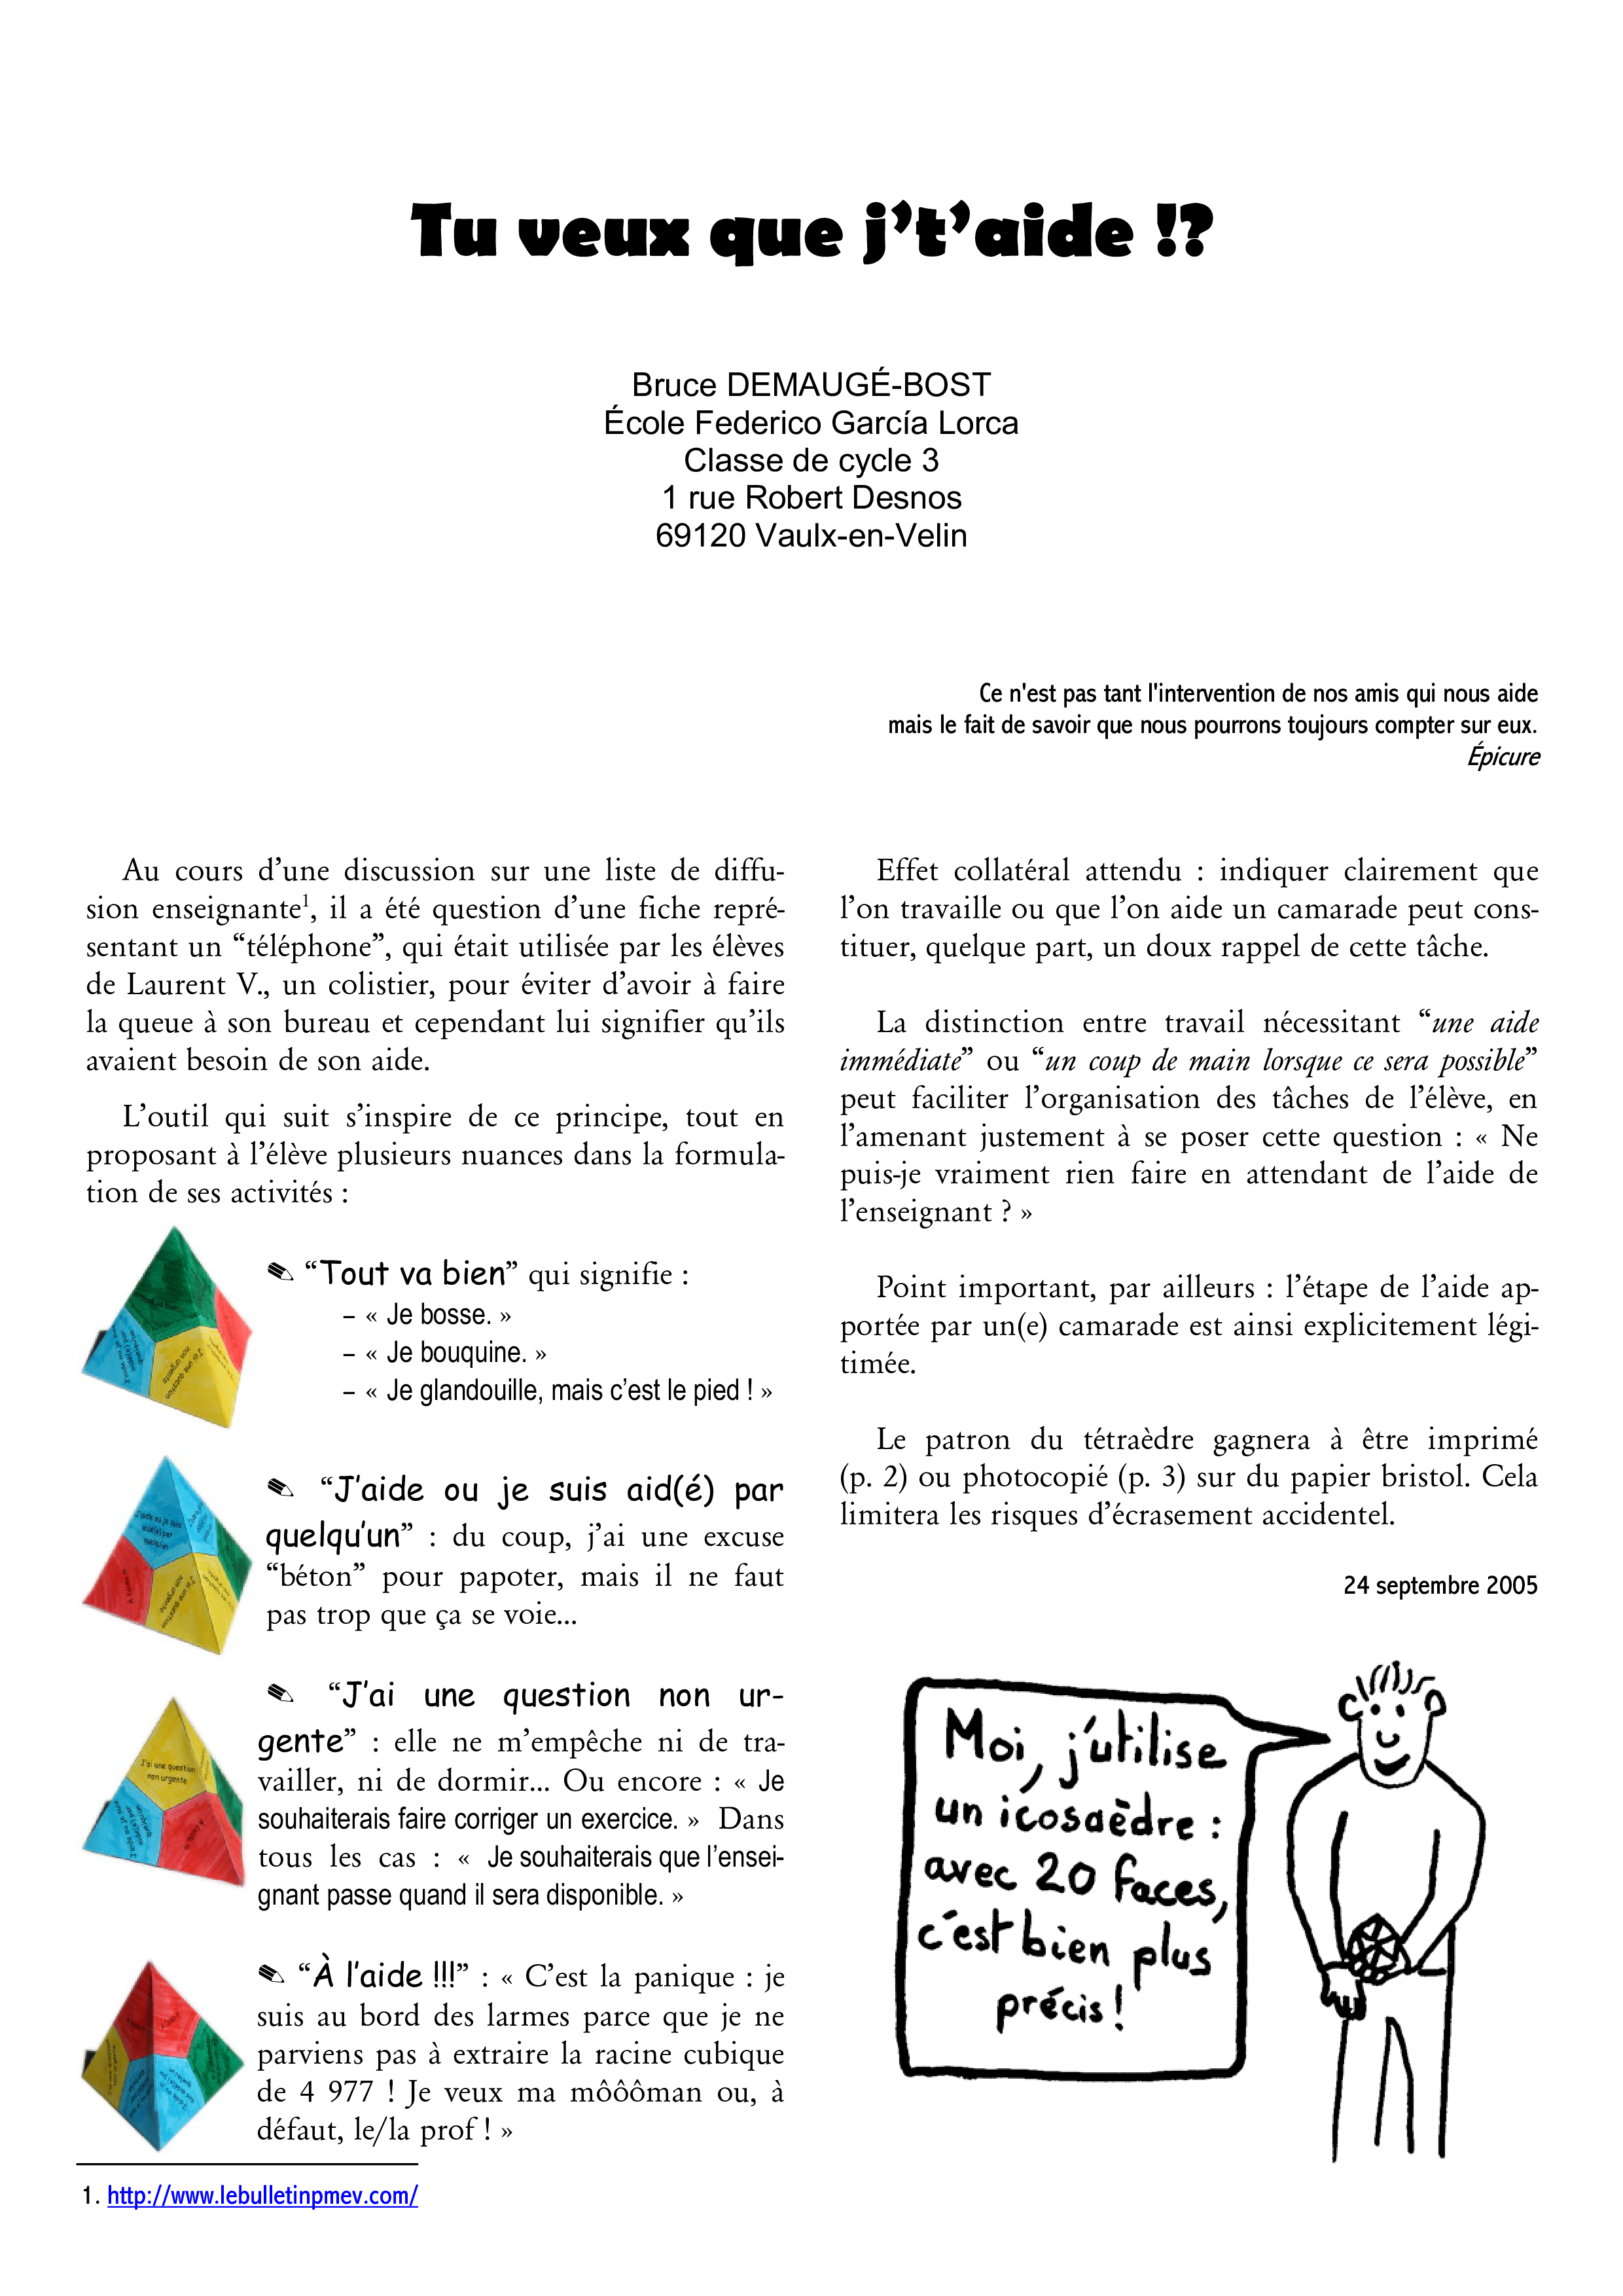
\includegraphics[scale=0.2]{annexes/01_tetraaide_0.png}
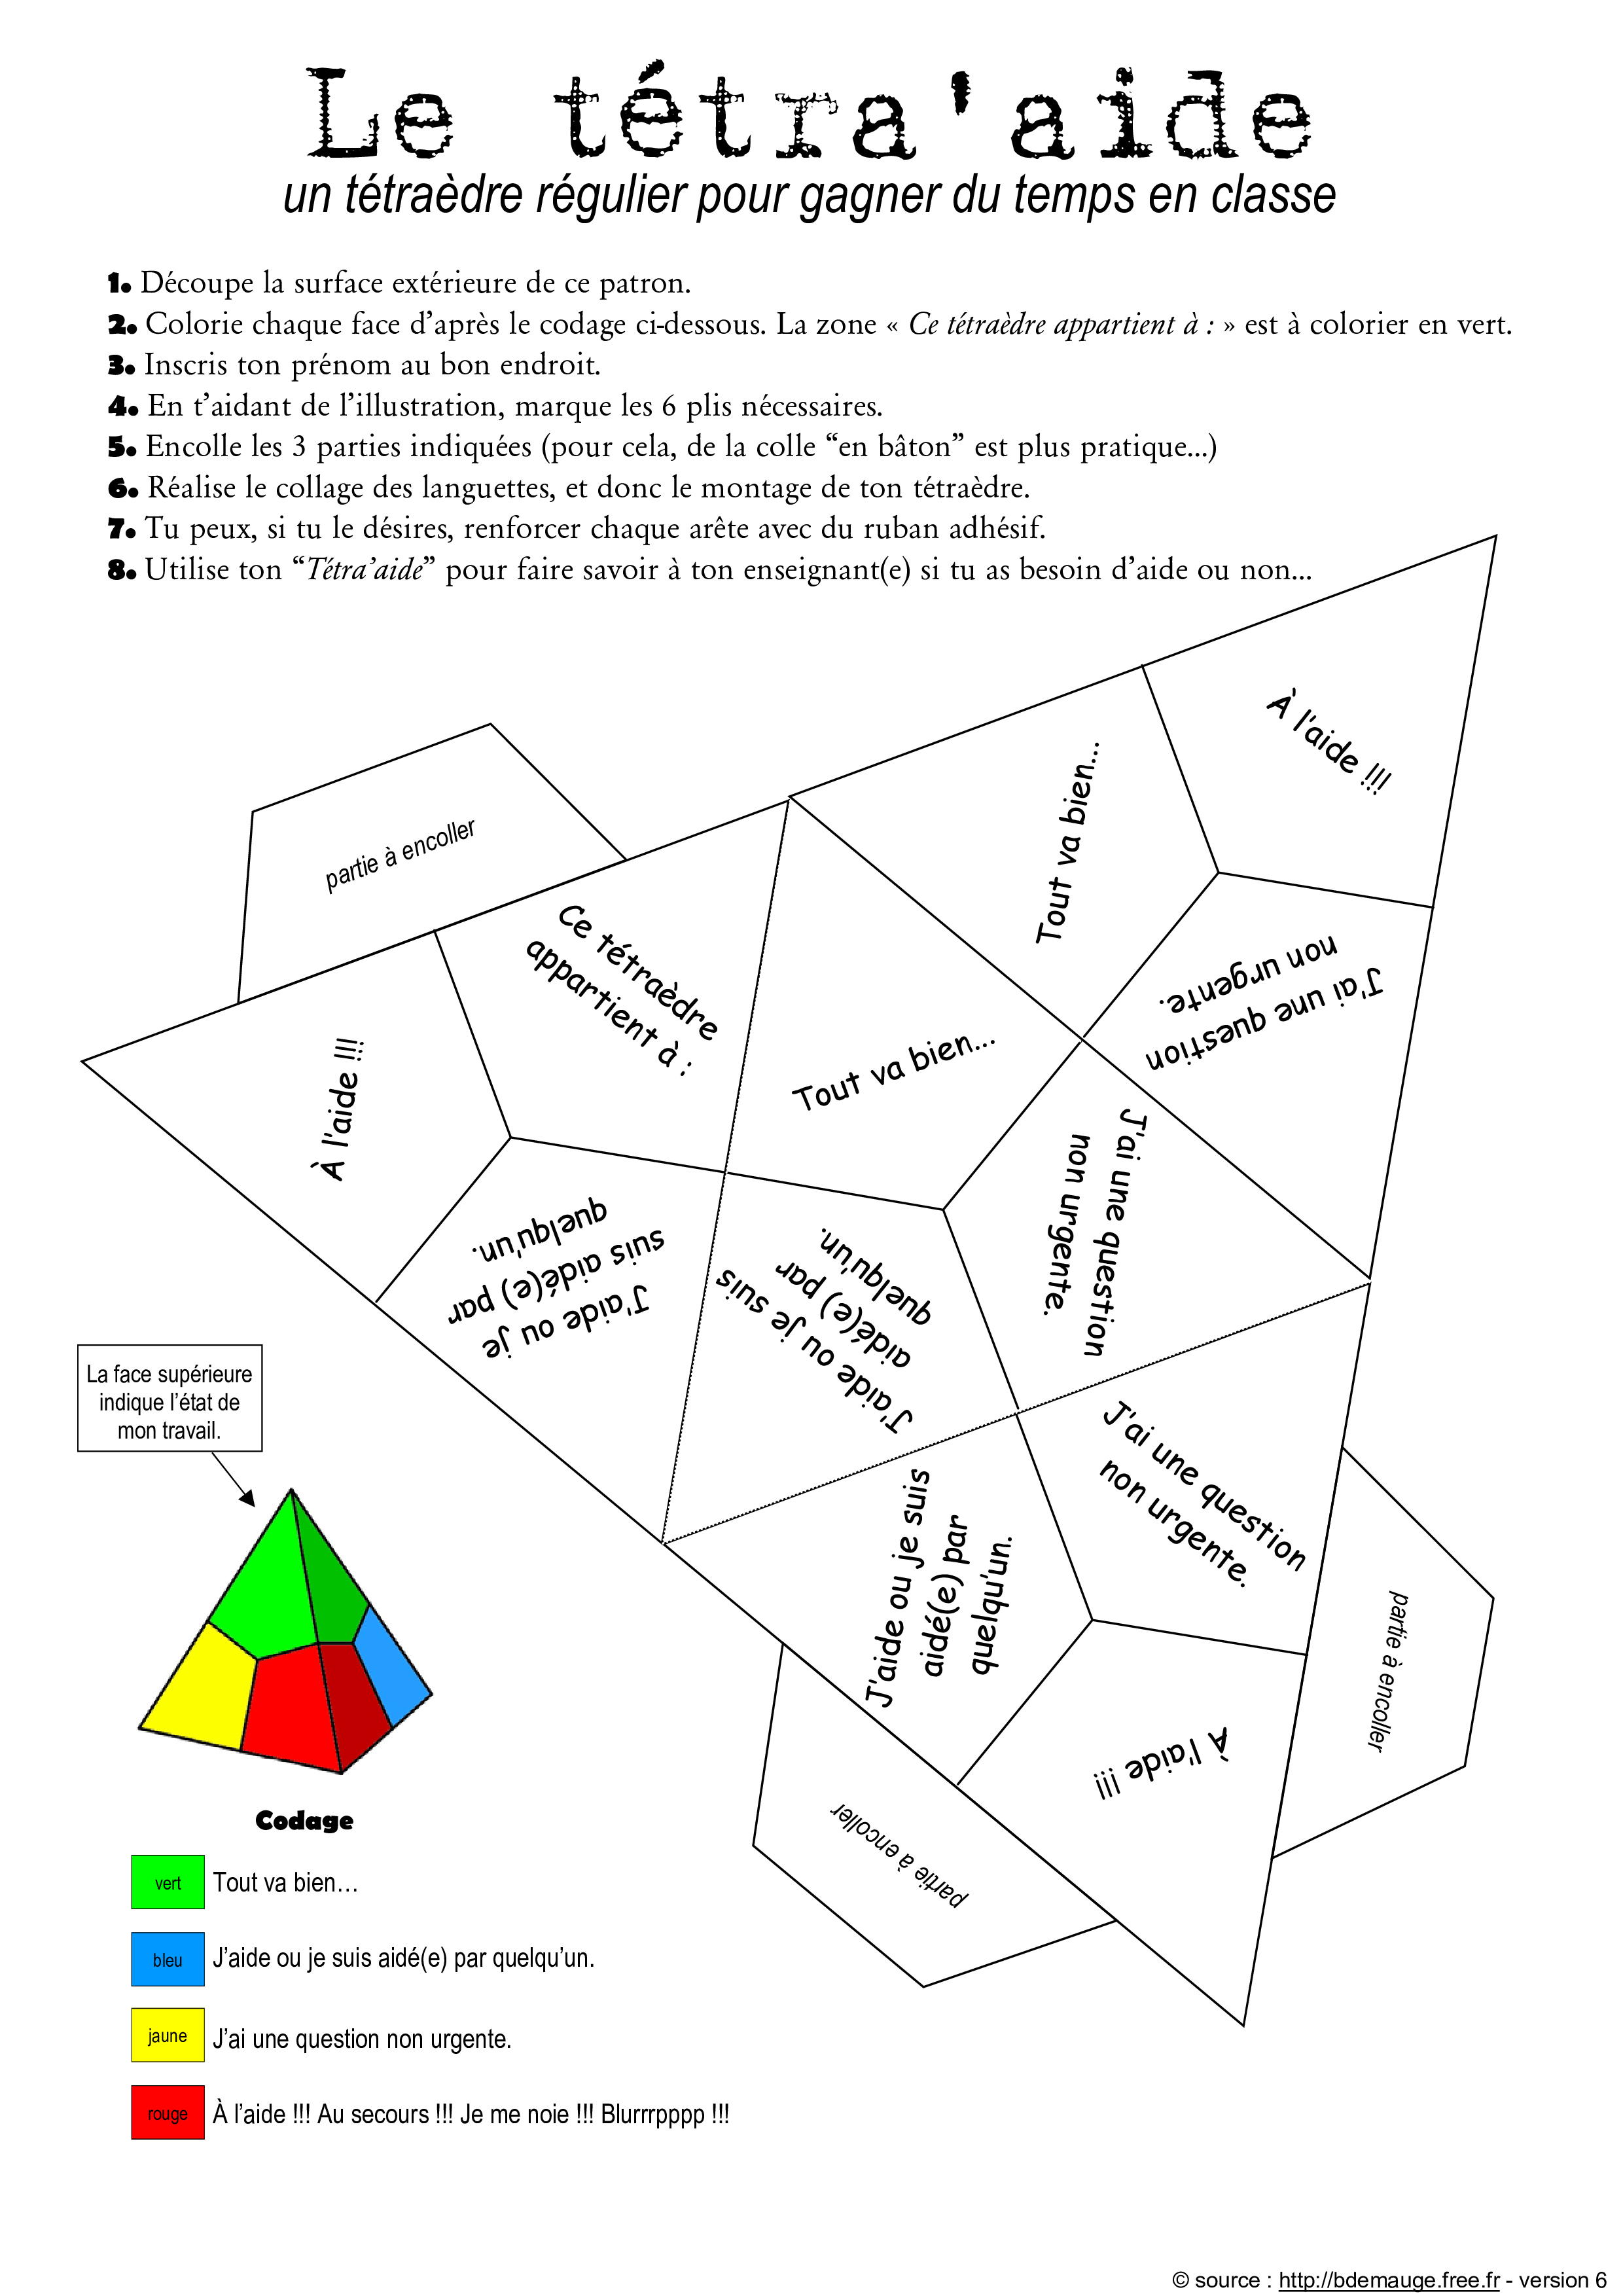
\includegraphics[scale=0.2]{annexes/01_tetraaide_1.png}
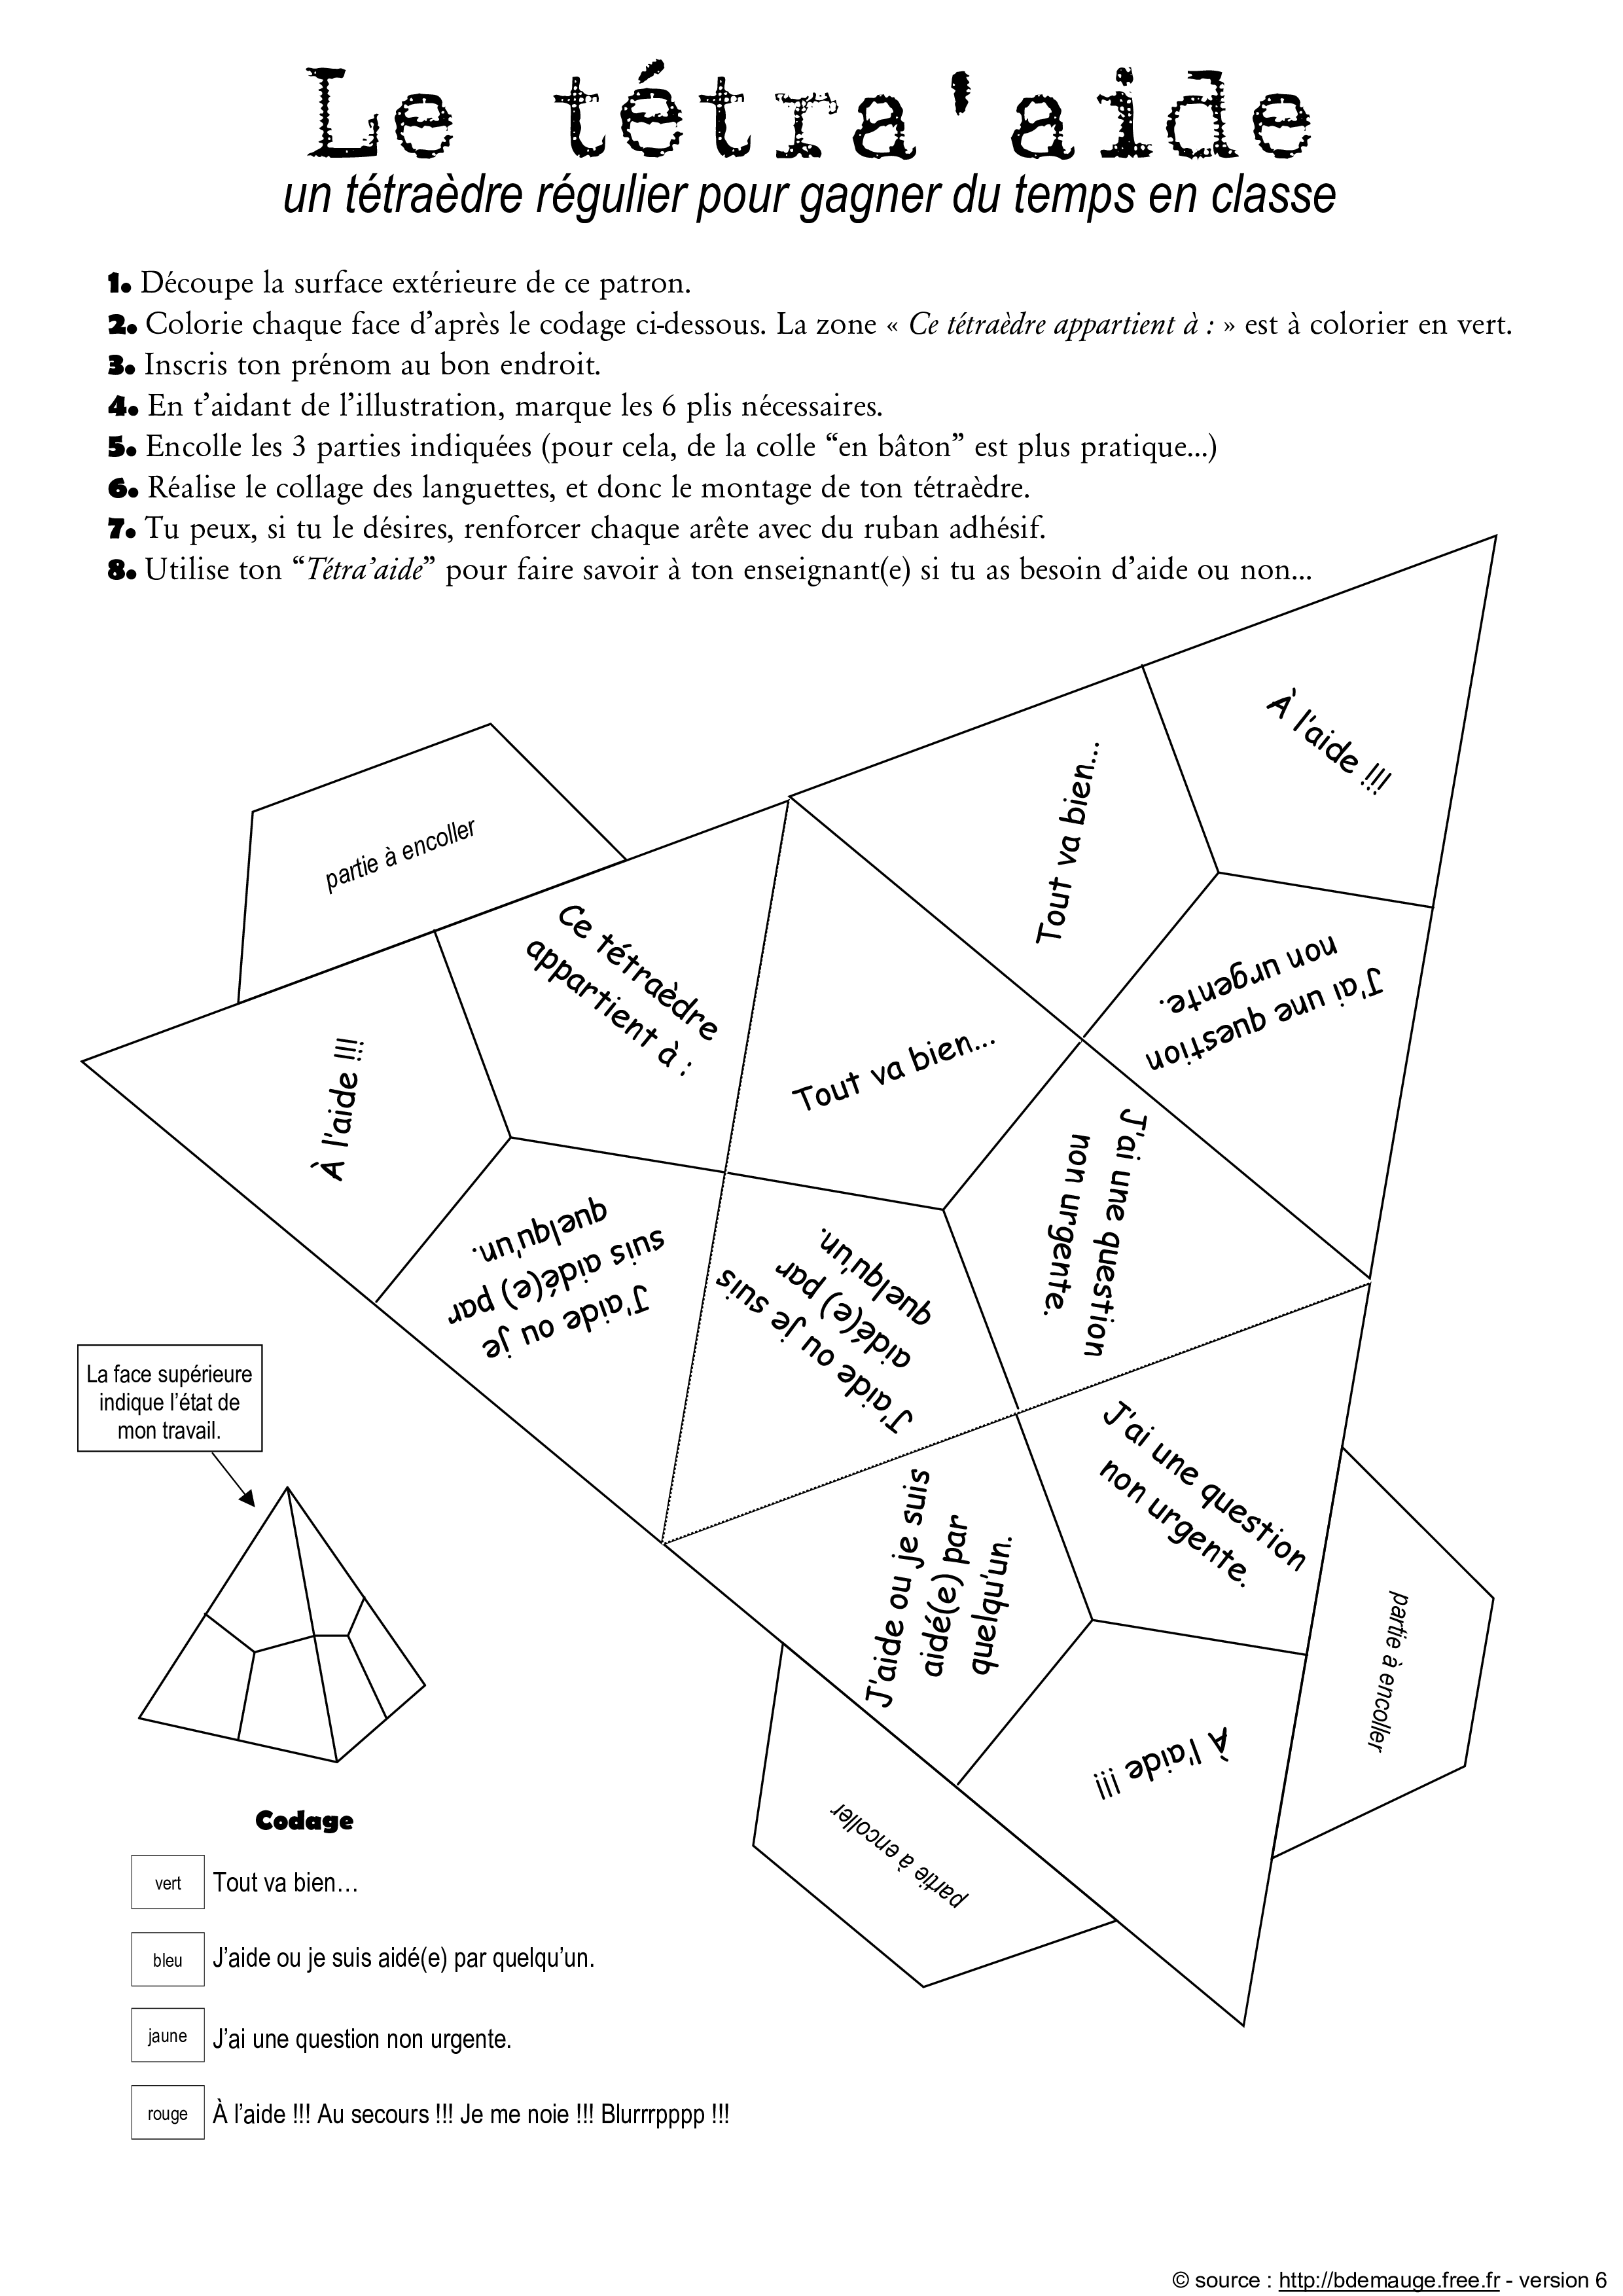
\includegraphics[scale=0.2]{annexes/01_tetraaide_2.png}
\end{center}

    \section{Sujet d'évaluation différenciée}\label{sujet_differencie}
\begin{center}
    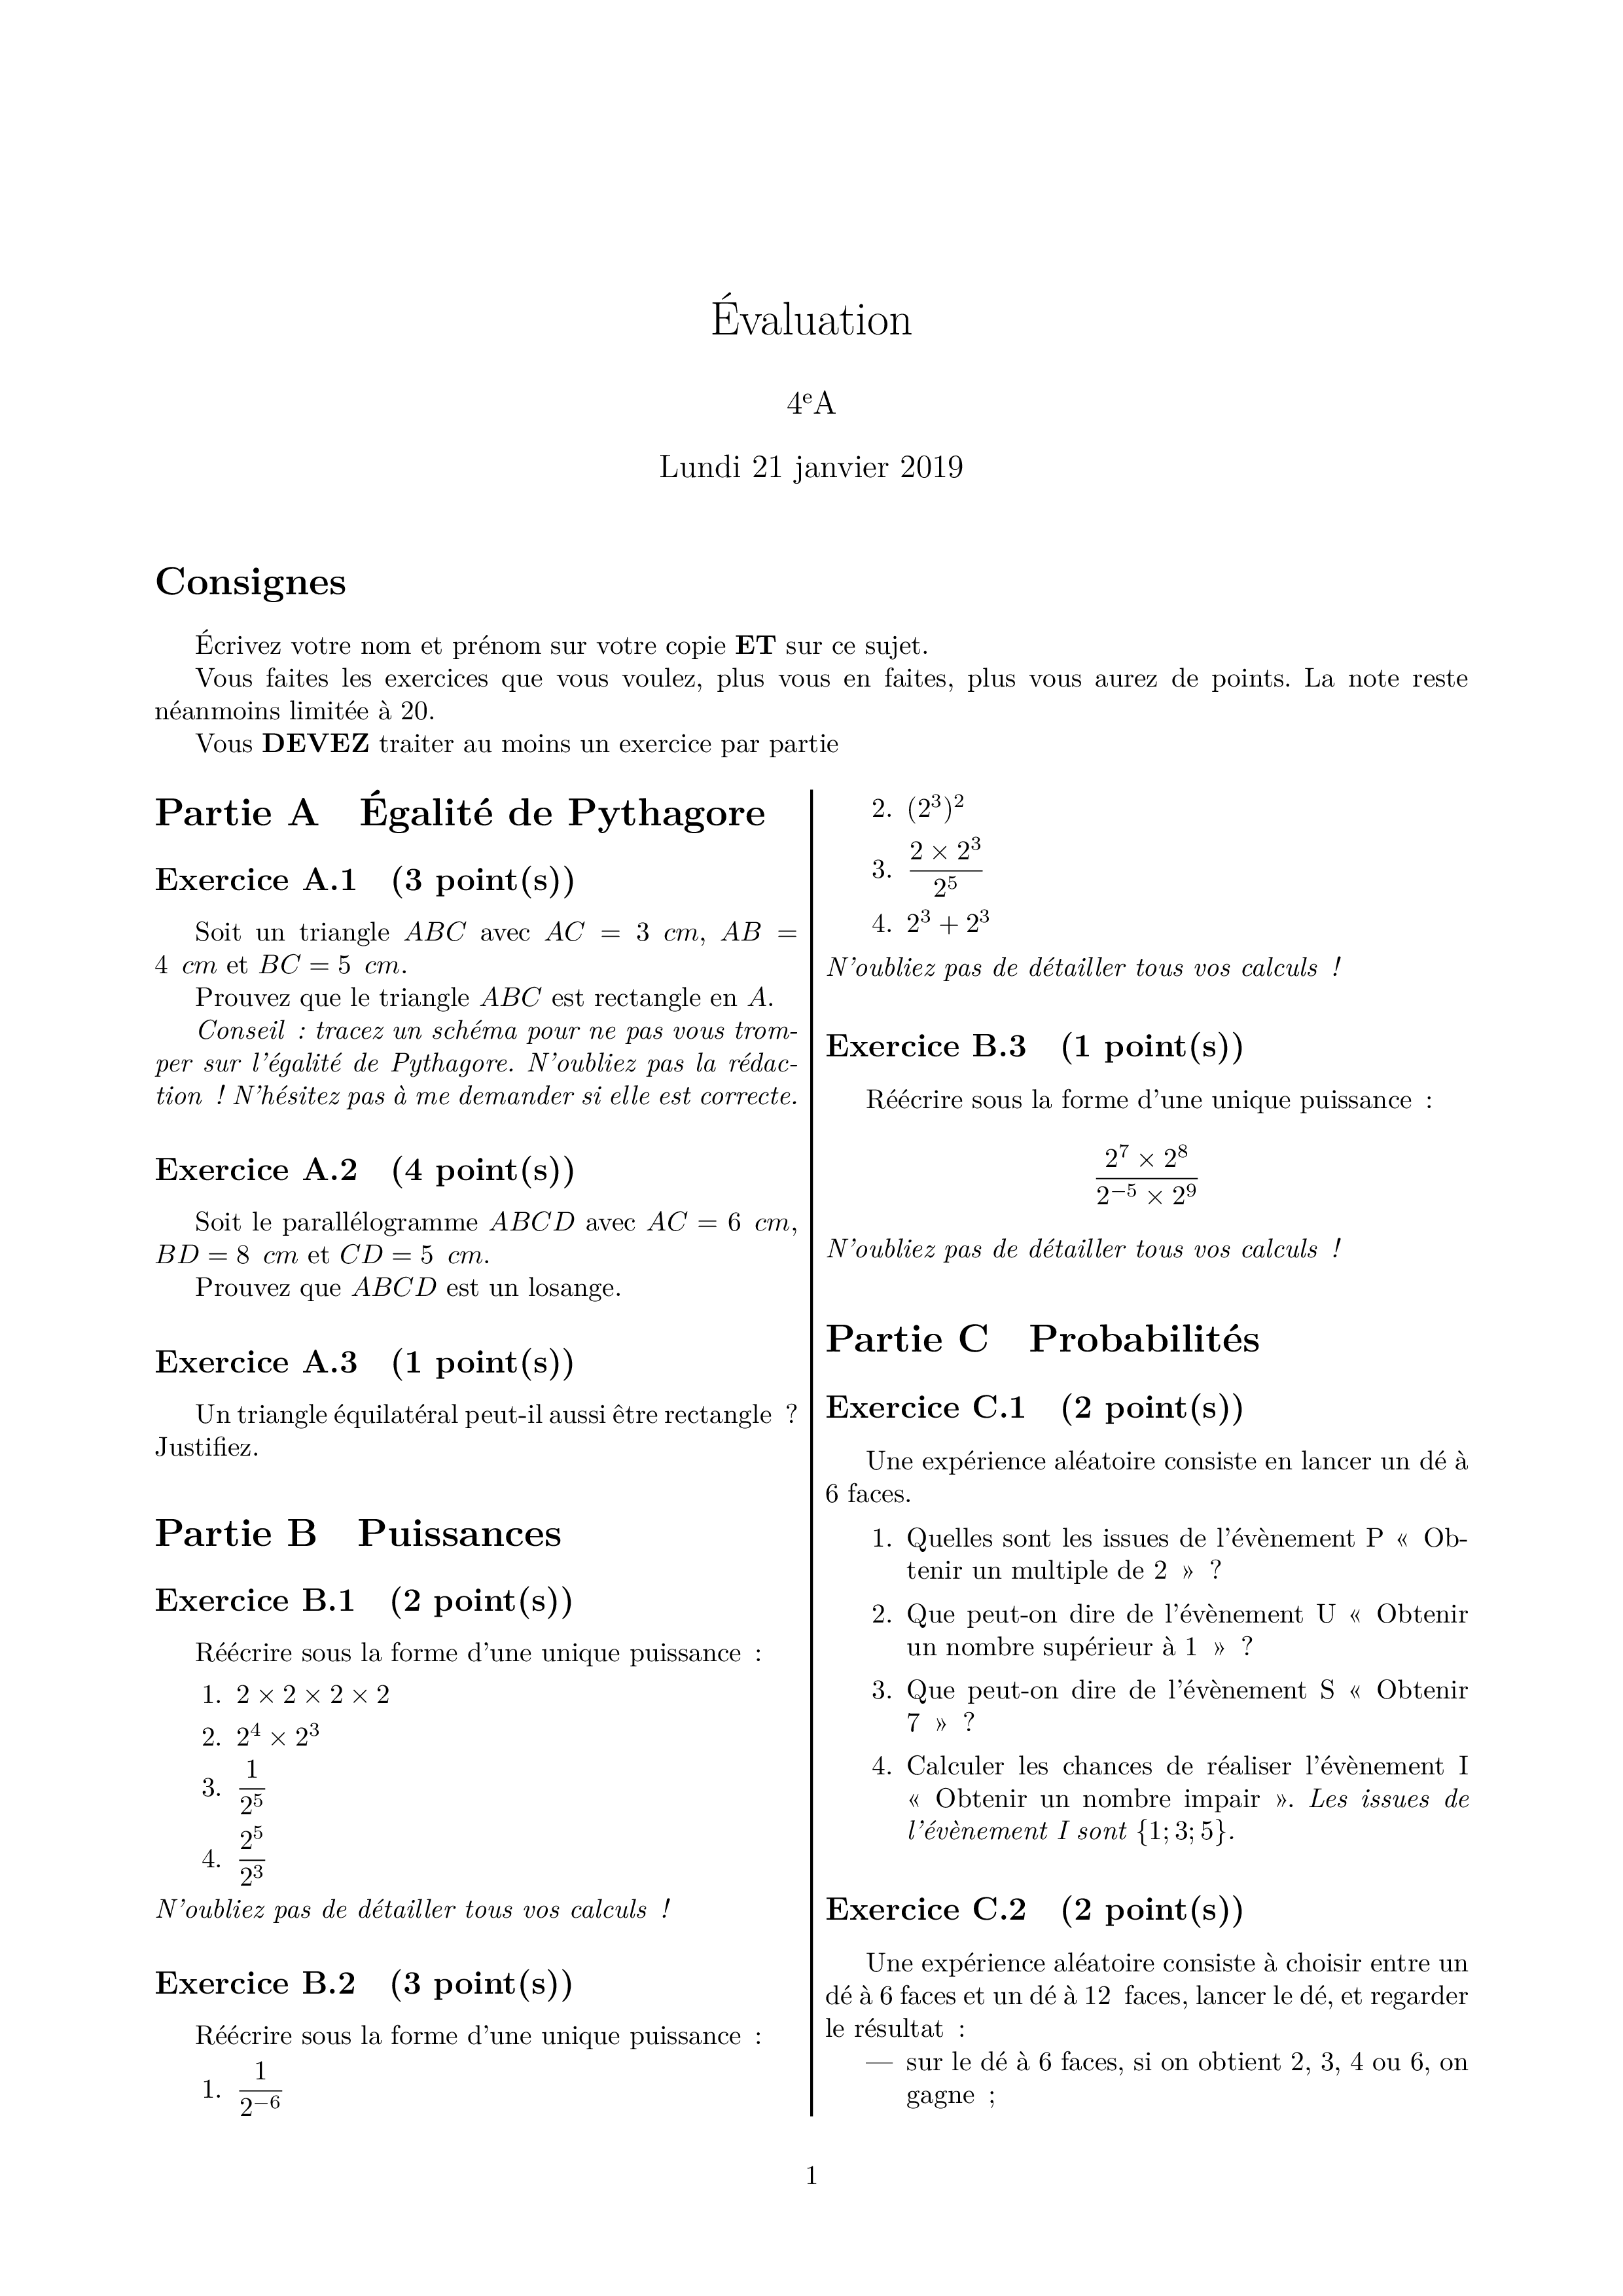
\includegraphics[scale=0.2]{annexes/sujet_differencie0.png}
    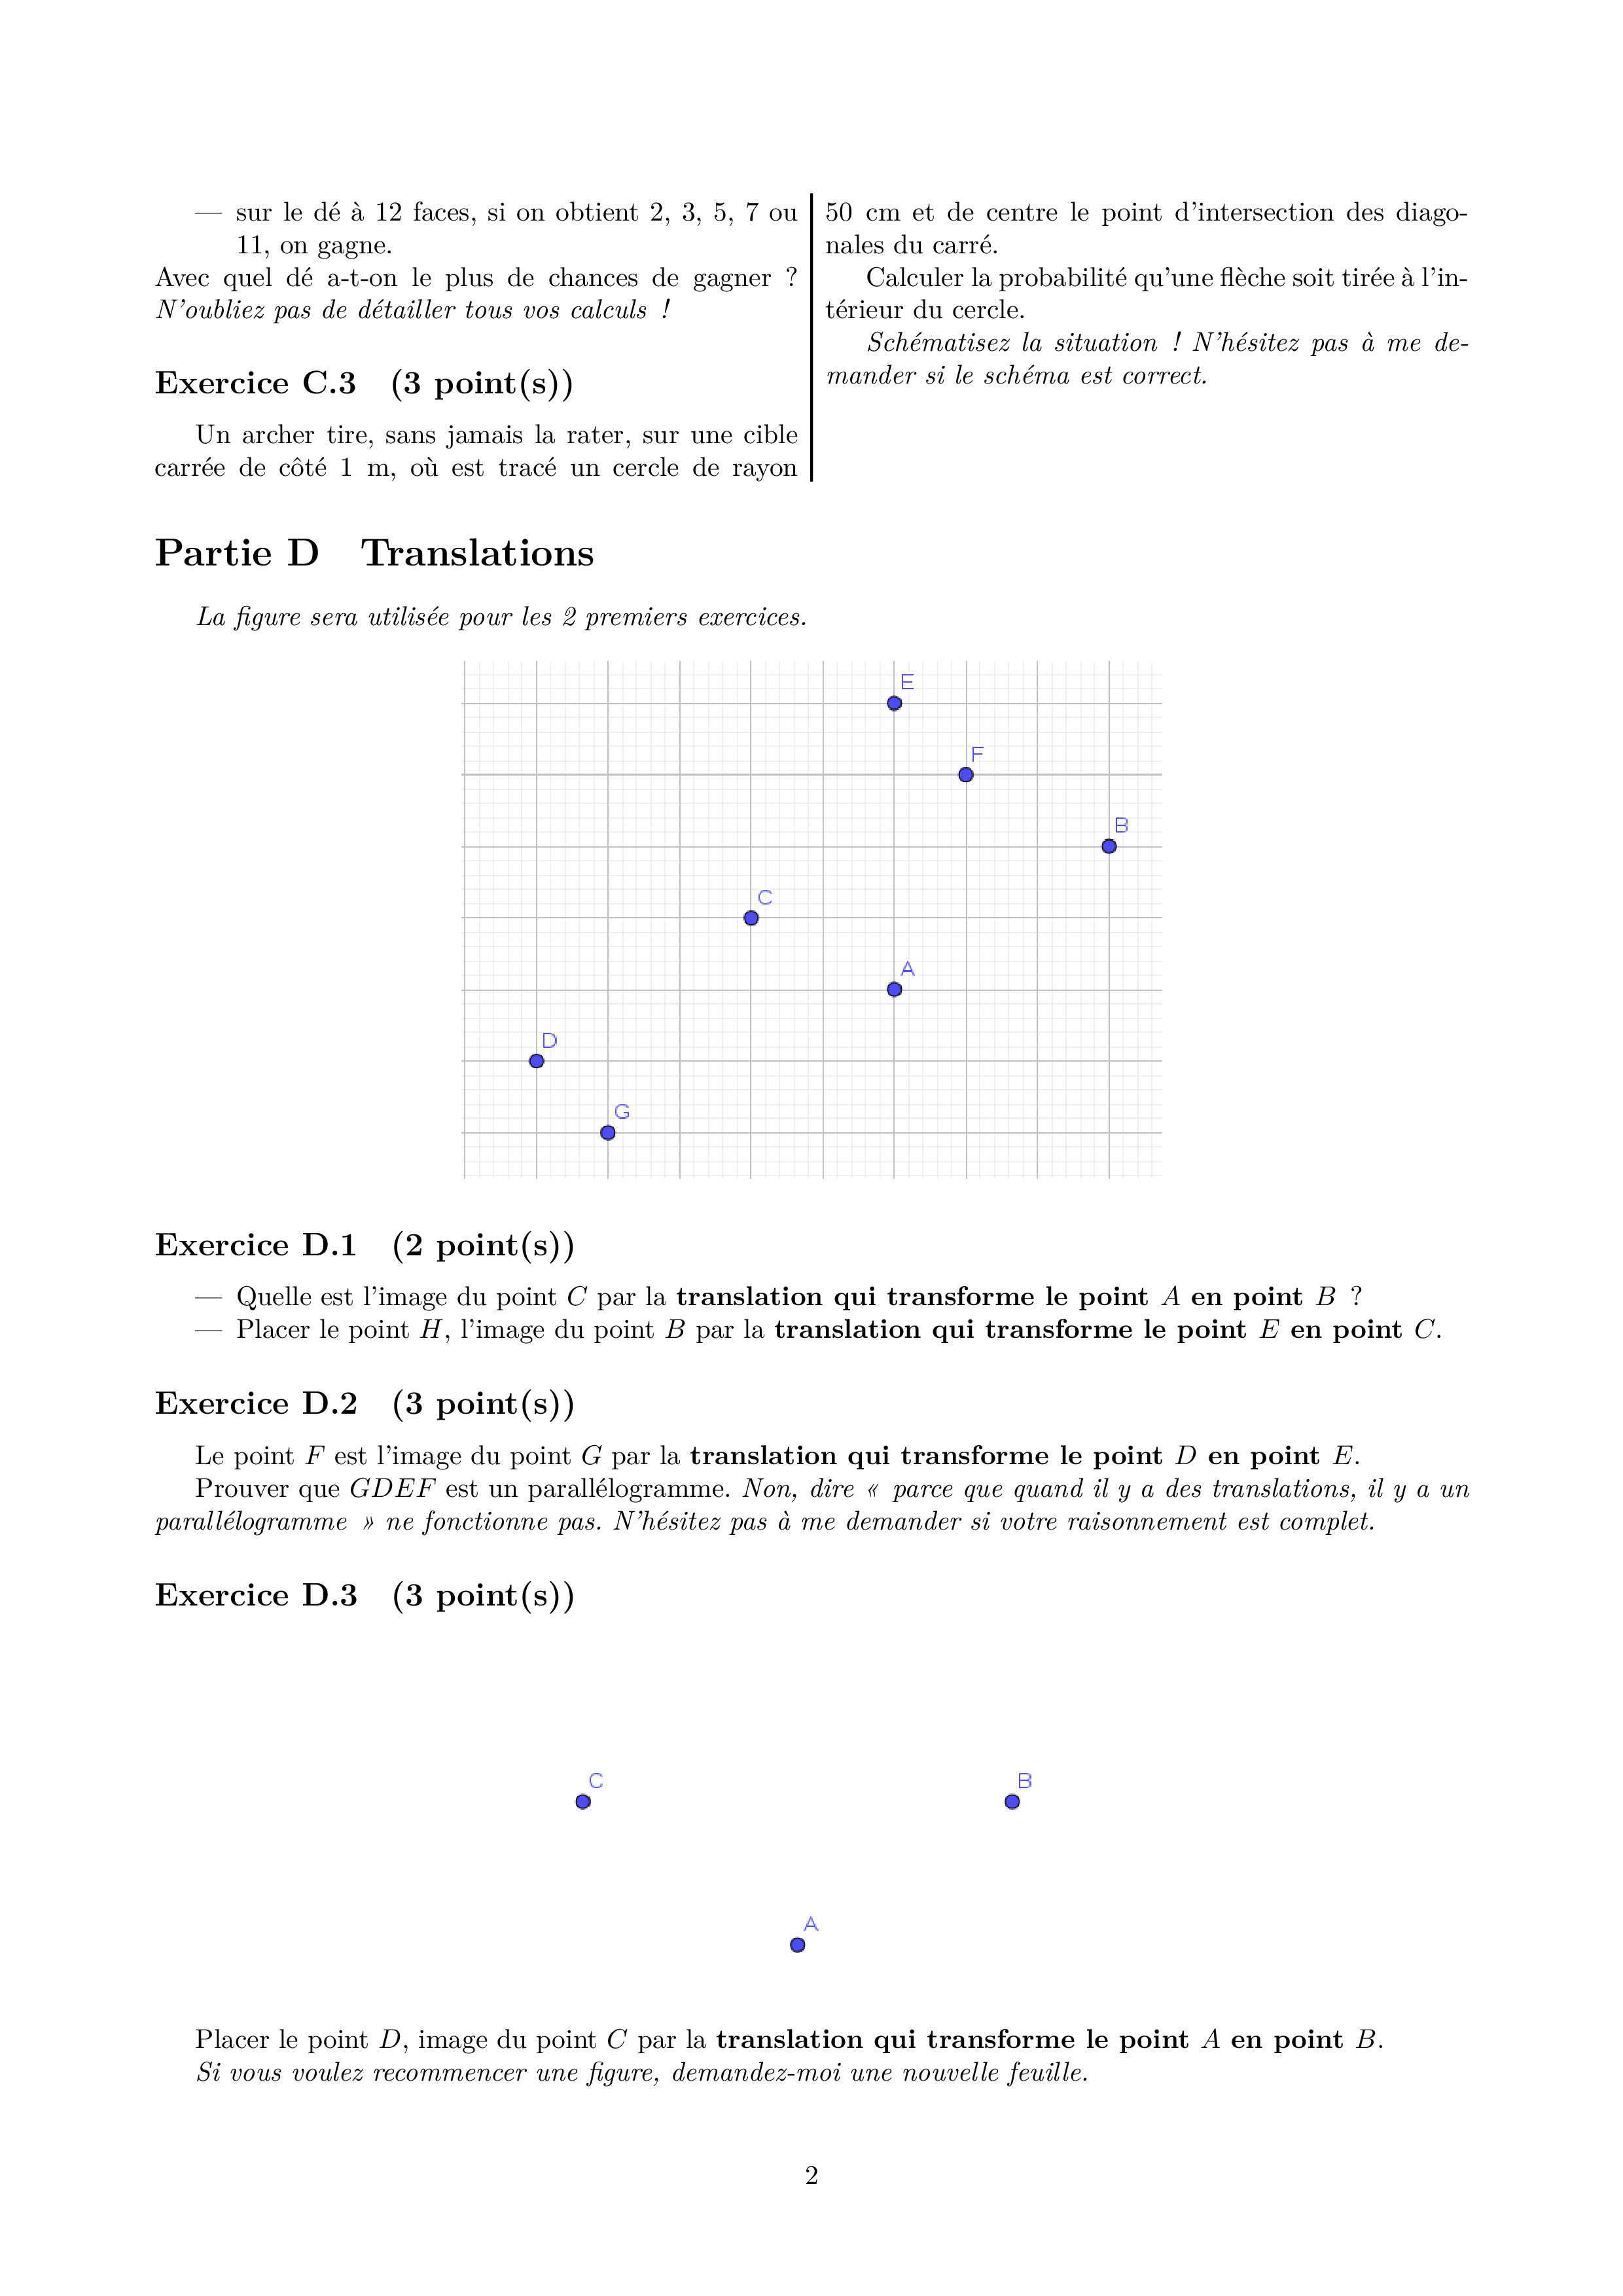
\includegraphics[scale=0.2]{annexes/sujet_differencie1.png}
\end{center}

    \begin{frame}
    \frametitle{Principe du parcours différenciés}
	Les élèves \textbf{effectuent à leur rythme} une série d'exercices \textbf{adaptés à leurs difficultés}.\\
	\vspace*{1.5cm}
	\textbf{insertion parcours différencié}\\
	Difficultés :
	\begin{itemize}
		\item Choix des exercices
		\item Fonctionnement en classe, gestion de la progressions
		\item Mise en place de \textit{balises}
	\end{itemize}
\end{frame}

\begin{frame}
	\frametitle{Construire un parcours différencié adapté}
	\vspace*{0.5cm}
	\'{E}tapes clefs de la construction du parcours différencié idéal :\\
	\begin{enumerate}
		\item \'{E}valuation diagnostique
		\item \'{E}laboration de cours ou aides sur divers supports
		\item Choix des exercices du parcours
		\item Choix du rythme des séances et des moments de reprise
		\item Construction des évaluations intermédiaire et sommative
	\end{enumerate}
\end{frame}

    \section{Différenciation pour la symétrie}

\subsection{Activité des cocottes}\label{annexe:symetrie-act}

Énoncé initial : Chacune des cocottes blanches a été obtenue à partir de la grise par une transformation différente.  Classe les couples de cocottes en fonction des transformations utilisées pour les construire.

\begin{figure}[h!]
    \centering
    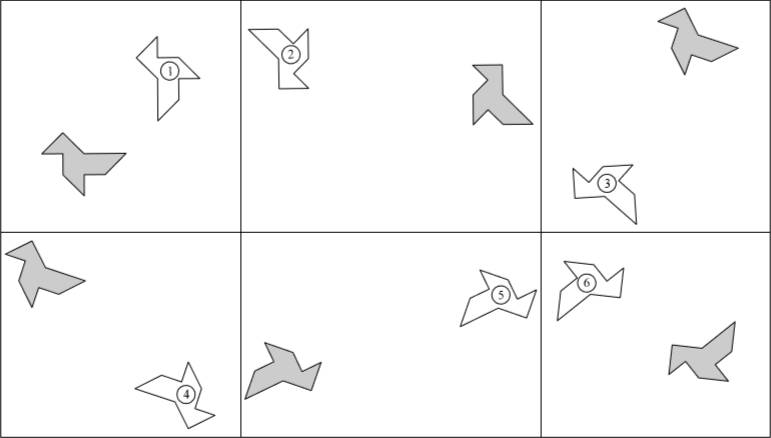
\includegraphics[width=0.9\linewidth]{img/activitemepcc.jpg}
    \caption{Source : \textit{Des maths ensemble et pour chacun 5\up{e}}}
    \label{fig:symetrie-act}
\end{figure}

\subsection{Fiches méthodologiques}\label{annexe:symetrie-fiches}

Les fiches méthodologiques sont scannées et présentes à cette adresse : \url{https://vvvictoire.github.io/memoire-meef/fiches-methodologiques.html}

\subsection{Activité en salle informatique}\label{annexe:symetrie-tice}

Pour cette séance, suite à plusieurs évaluations diagnostiques ponctuelles, j'avais décidé de retravailler la symétrie axiale et la symétrie centrale. L'objectif de cette séance est donc de leur permettre de consolider l'image mentale qu'ils se font des symétries en travaillant chez eux sur GeoGebra pendant les vacances. Pour cela, je leur ai préparé un exercice à réaliser seul sur GeoGebra pour se familiariser avec le logiciel et pour apprendre à s'auto-évaluer avant de refaire les activités seul à la maison.

Le fichier GeoGebra contient trois lettres dont les élèves devaient tracer le symétrique (par rapport à un point et par rapport à une droite). Dans un premier temps, ils devaient tracer le symétrique sur fond blanc et dans un deuxième temps en s'aidant du quadrillage. Enfin, ils devaient placer les axes de symétrie et les centres de symétrie de chaque lettre.

GeoGebra avait déjà été montré aux élèves comme un \textit{outil de conjecture}. Dans cette séance, c'est la première fois qu'ils utilisaient Gogebra en tant qu'\textit{outil de contrôle et de remédiation}. J'avais particulièrement insisté sur l'utilisation de l'outil \textit{Symétrie axiale} et de l'outil \textit{Symétrie centrale} comme \textbf{moyens de vérification} et non comme aides visuelles.

L'analyse complète de la séance, la fiche élève et le fichier GeoGebra associé sont disponibles à cette adresse : \url{https://vvvictoire.github.io/memoire-meef/extraits-de-portfolio.html}

\subsection{Analyse d'évaluation portant sur la symétrie}\label{annexe:symetrie-eval}

Dans un exercice de cette évaluation, les élèves devaient préciser la méthode employée pour construire le symétrique d'une ligne brisée connaissant l'emplacement d'un des segments du symétrique.

\begin{figure}[h!]
    \centering
    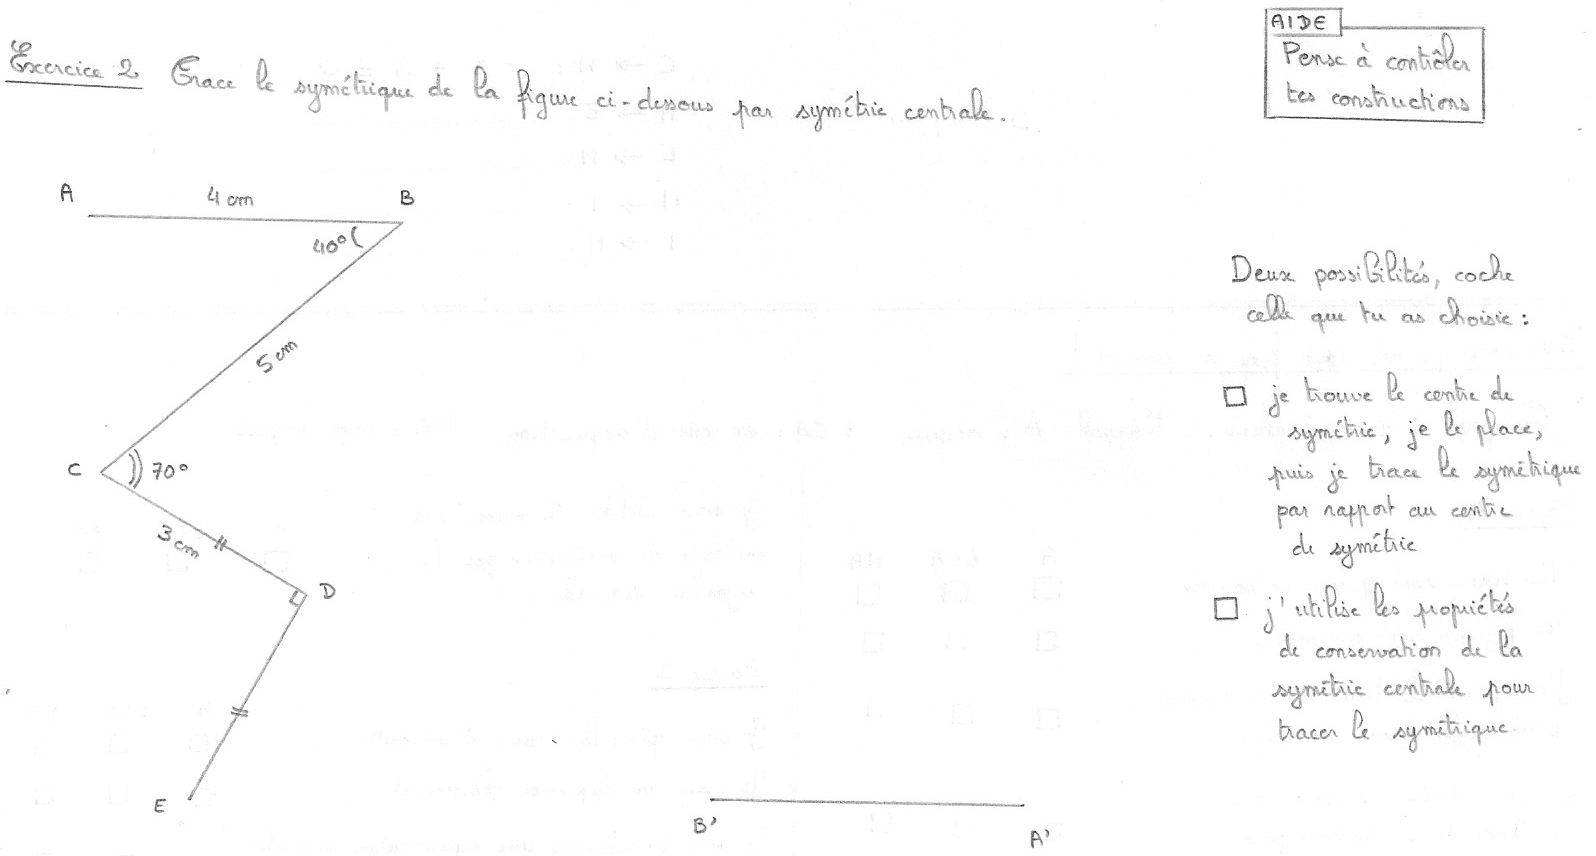
\includegraphics[width=\linewidth]{img/page1-exo2.png}
    \caption{Les propriétés de conservation de la symétrie centrale venaient d'être vues, peu d'élèves avaient eu le temps de se les approprier.}
    \label{fig:xav-eval}
\end{figure}

En dehors des évaluations à joker et des évaluations adaptées à un élève Italien en difficulté avec la langue française, ceci est la seule question différenciée proposée dans toutes mes évaluations. Cela n'est pas clairement précisé dans l'analyse de cette évaluation, mais il est important de préciser que cette question n'apportait pas de point pour la note chiffrée, bien qu'elle apparaisse dans la grille d'évaluation par compétences.

L'analyse complète de l'évaluation est disponible à cette adresse : \url{https://vvvictoire.github.io/memoire-meef/extraits-de-portfolio.html}

\clearpage

\section{Différenciation pour les angles alternes-internes}

\subsection{Évaluations diagnostiques}\label{annexe:angles-prod1}

Voici quelques citations extraites de copies d'élèves. La question initiale était : \og Quelle est la définition d'un angle alterne-interne ? \fg{}
\begin{itemize}
\item Deux droites parallèles coupées par une droite sécante [donnent des angles] alternes internes de même mesure (confusion entre définition et propriété)
\item Alterne : angle à l'extérieur de la droite qui coupe les deux droites parallèles. Interne : angle à l'intérieur de la droite qui coupe les deux droites parallèles.
\item Quand il y a deux droites parallèles coupées par une droite sécante, les deux angles sont à l'intérieur et disposés de part et d'autre de la sécante.
\item C[e sont] deux droites parallèles qui sont tranchées par une autre droite.
\end{itemize}

Sur nombre de copies, les élèves ont répondu à la deuxième question (\og Dessinez une figure où vous indiquerez les deux paires d'angles alternes-internes \fg{}) par un schéma comportant deux droites parallèles (bien qu'aucun élève ne précise explicitement que les droites sont parallèles). Un seul élève a tracé des droites non parallèles et un élève a produit ceci :

\begin{figure}[h!]
    \centering
    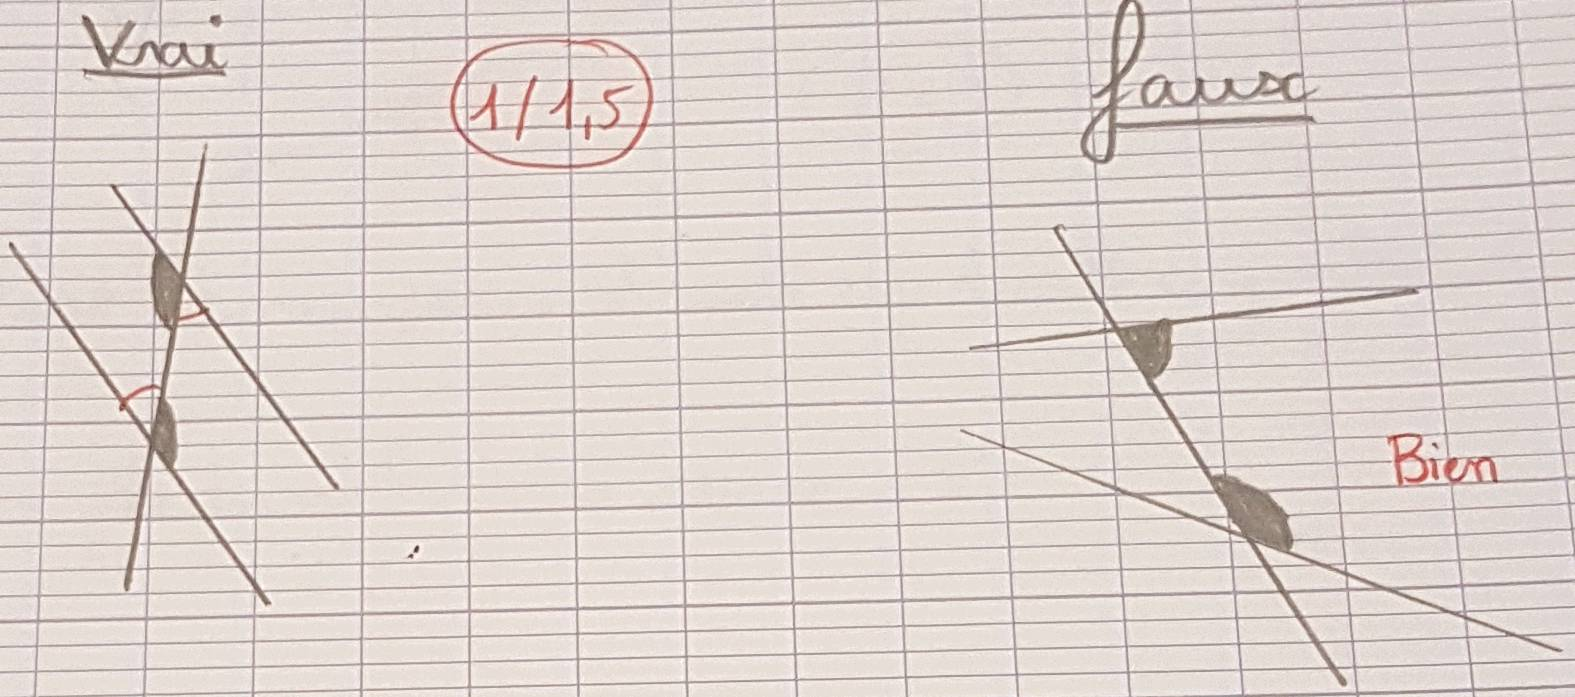
\includegraphics[width=0.6\linewidth]{img/anglesquestion.jpg}
    \caption{Associe-t-il la condition de droites parallèles à la définition des angles alternes-internes ou est-ce un hasard ?}
\end{figure}

Les captures d'écran associées à ces citations sont consultables à cette adresse : \url{https://vvvictoire.github.io/memoire-meef/angles-productions-d-eleves.html}

\clearpage

\subsection{Fiches d'exercice}\label{annexe:angles-fiches}

\begin{figure}[h!]
    \centering
    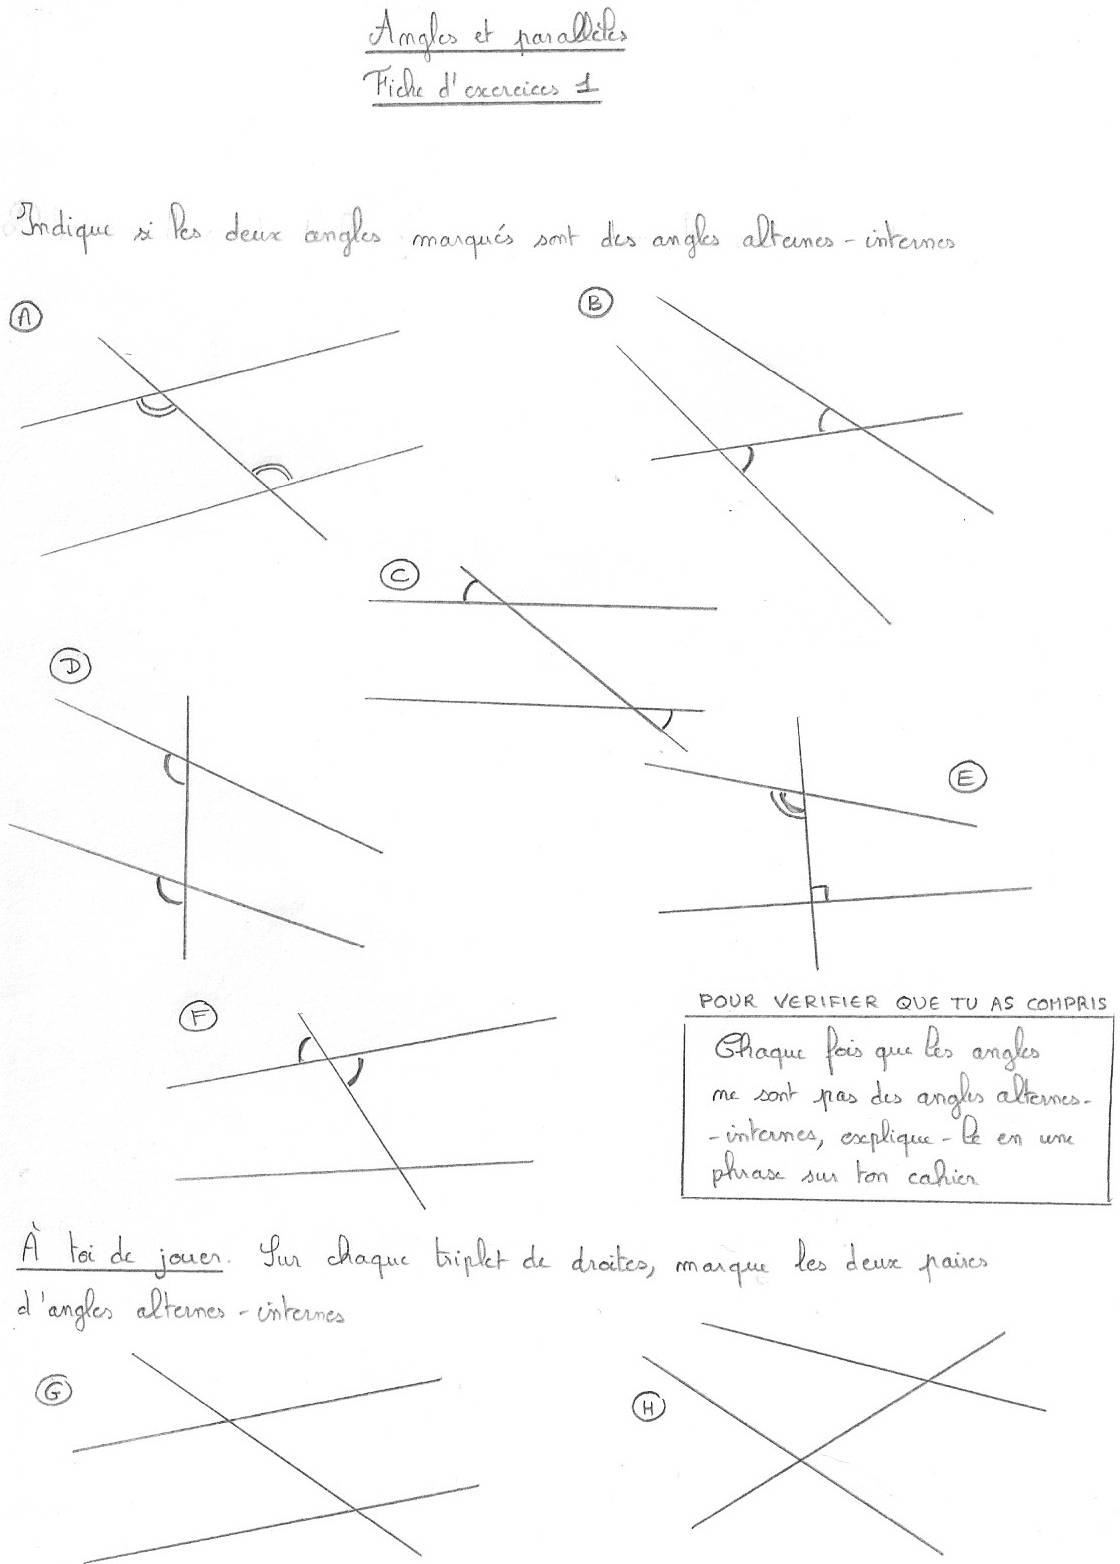
\includegraphics[width=0.6\linewidth]{img/anglesfiche1.jpg}
    \caption{Reconnaissance d'angles alternes-internes (cette feuille a fait l'objet d'une évaluation diagnostique). L'exercice supplémentaire n'a pas été traité.}
    \label{fig:angles-fiche1}
\end{figure}

\begin{figure}[h!]
    \centering
    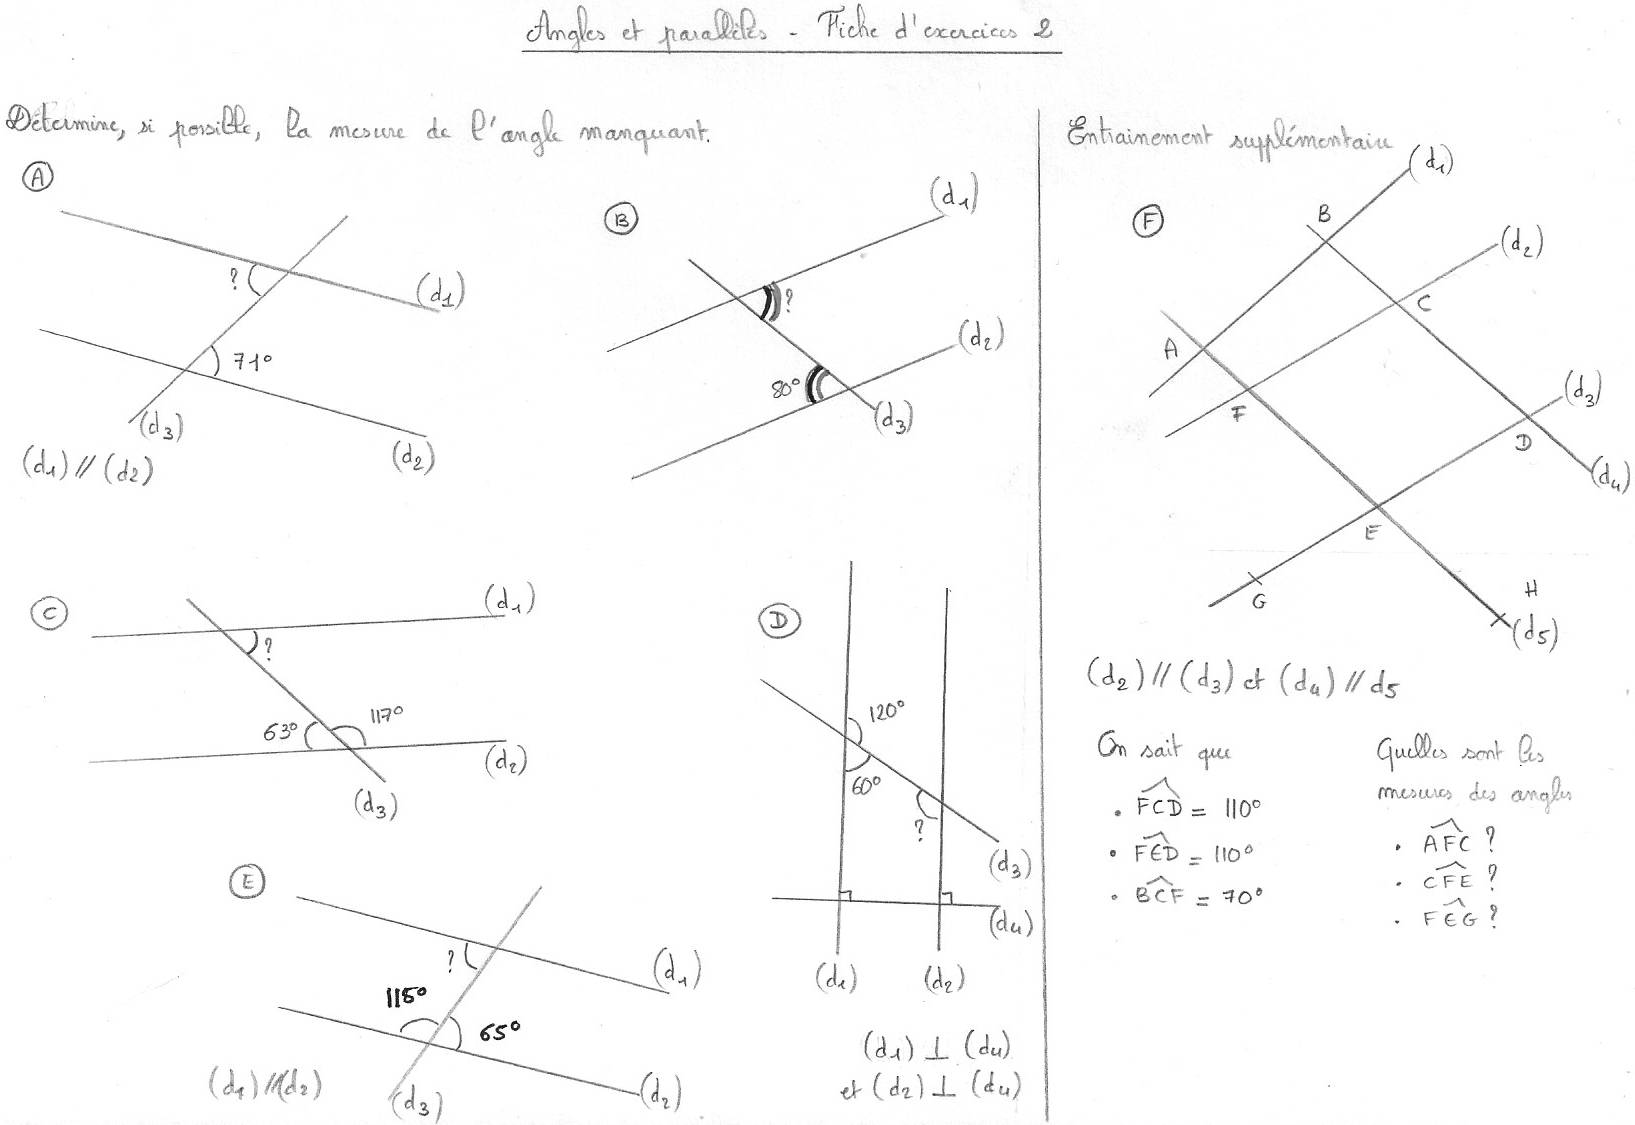
\includegraphics[width=0.8\linewidth]{img/anglesfiche2.jpg}
    \caption{Détermination de la valeur de l'angle par application directe de la propriété. Difficulté liée à la géométrie abstraite : les élèves doivent tenir compte des codages. Un exercice supplémentaire pour les élèves en avance.}
    \label{fig:angles-fiche2}
\end{figure}

\begin{figure}[h!]
    \centering
    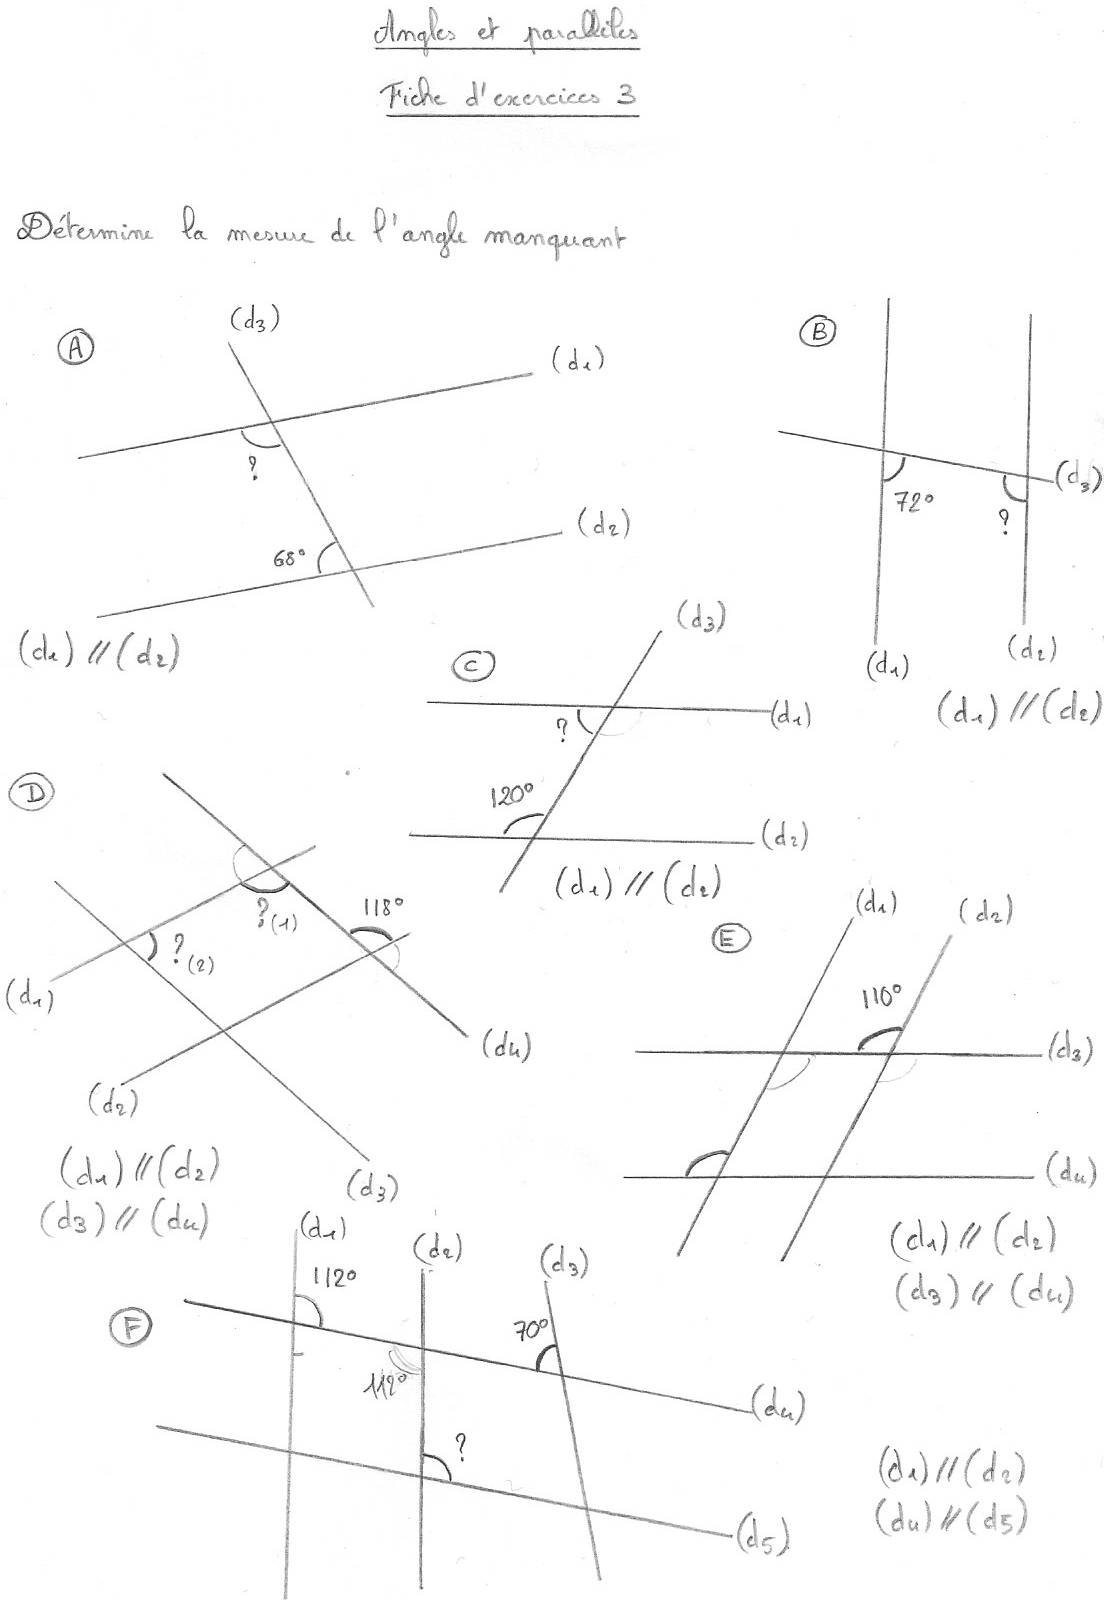
\includegraphics[width=0.6\linewidth]{img/anglesfiche3.jpg}
    \caption{Détermination de la valeur de l'angle soit par application directe de la propriété, soit par calcul du supplémentaire. Les schémas D, E et F étaient réservés aux élèves en avance.}
    \label{fig:angles-fiche3}
\end{figure}

\clearpage

\subsection{Histoire de la coccinelle et de la libellule}\label{annexe:angles-prod2}

\begin{figure}[h!]
    \centering
    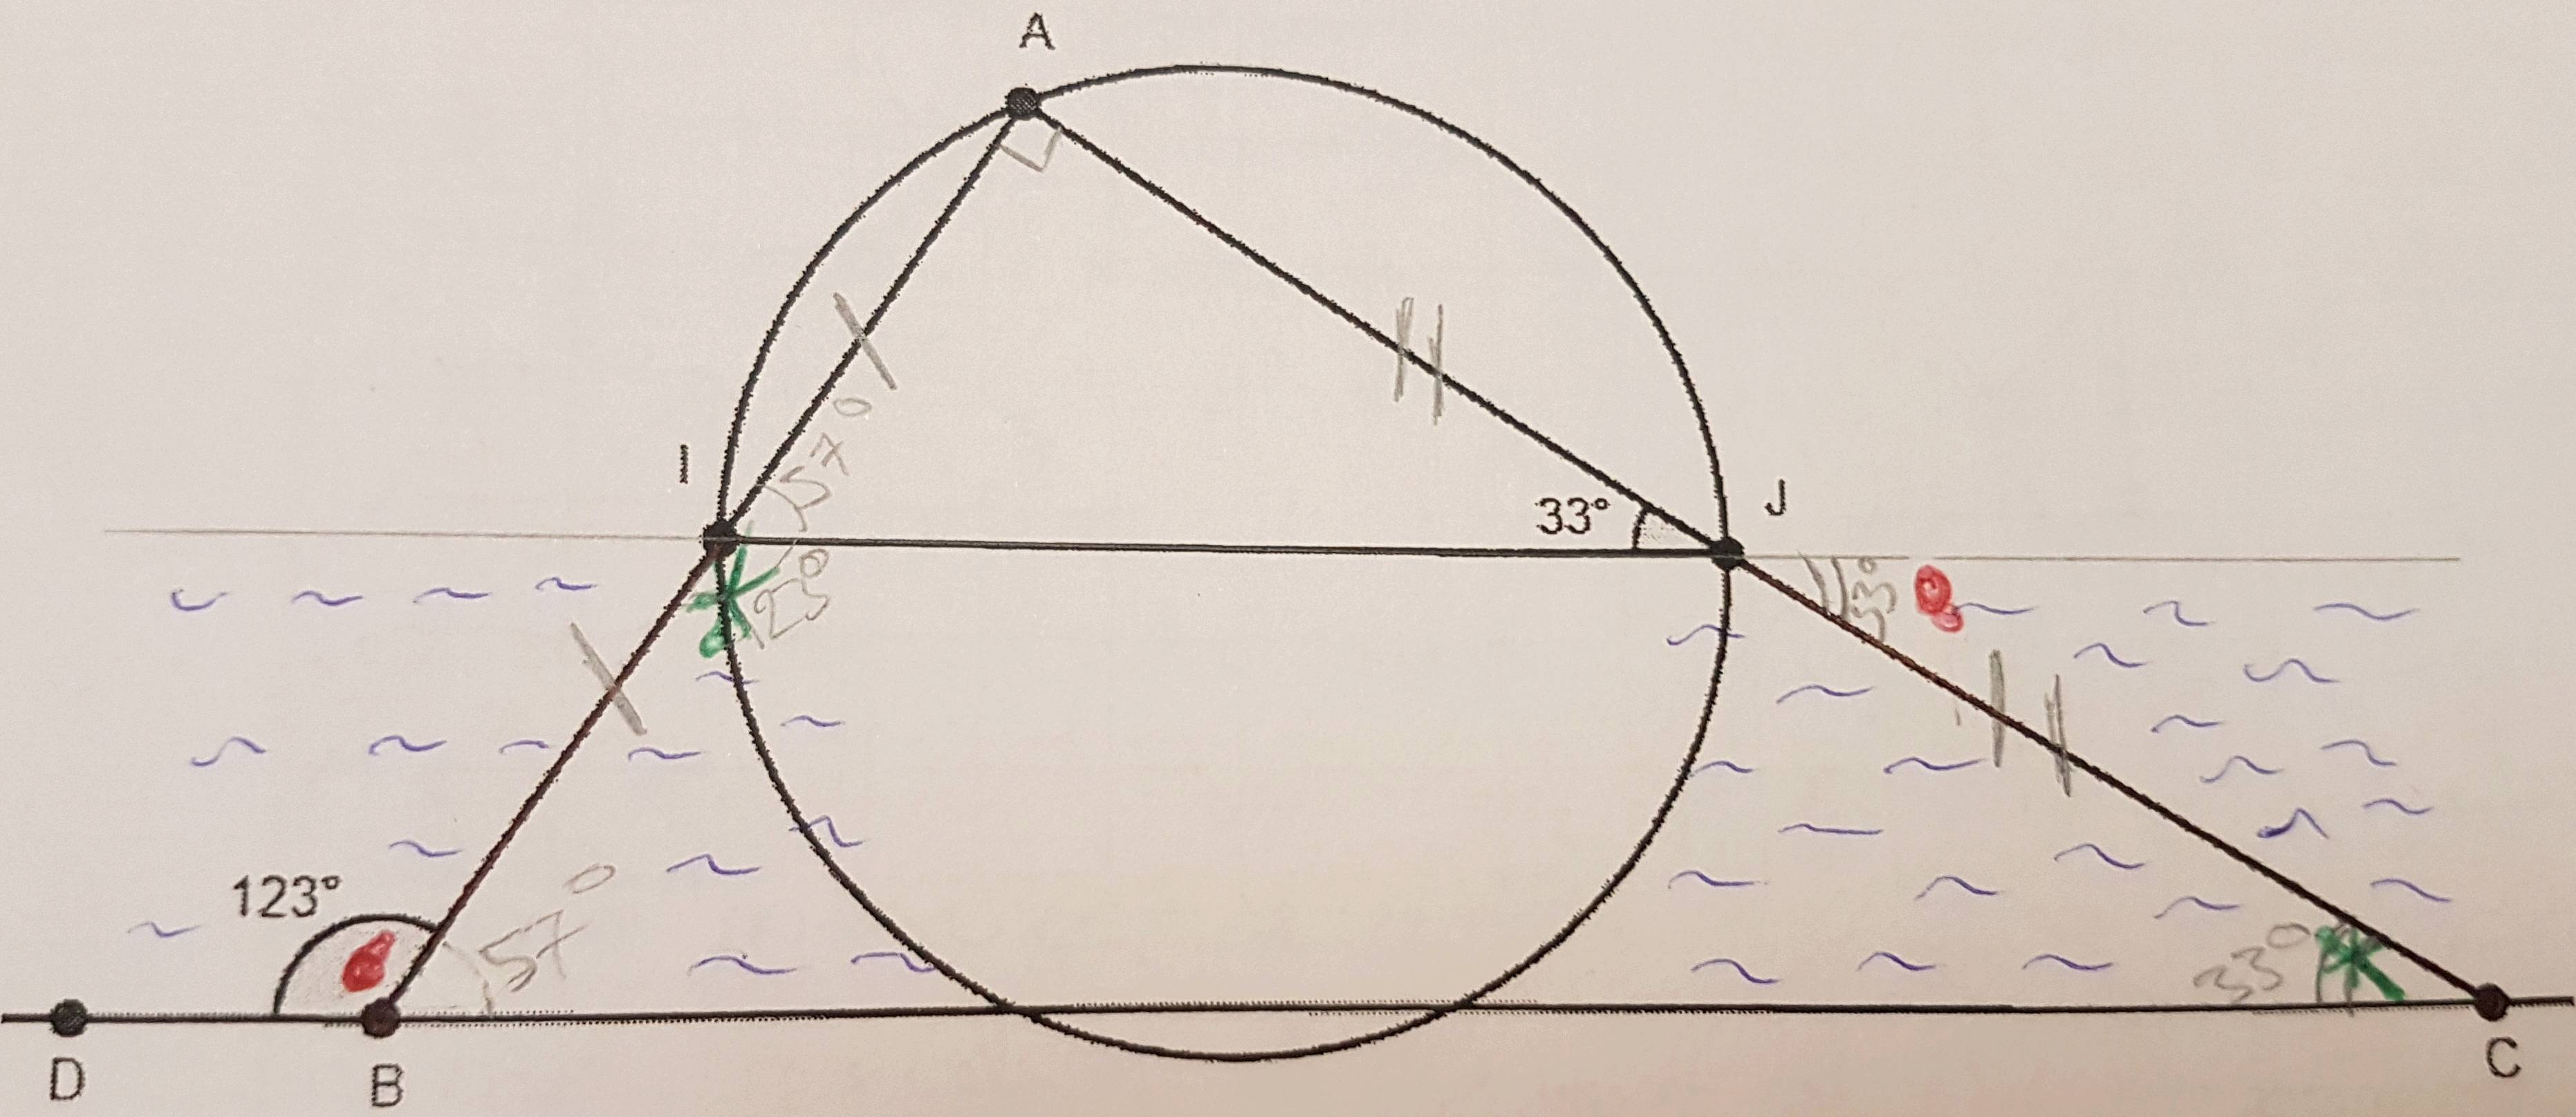
\includegraphics[width=\linewidth]{img/insectes-point.jpg}
    \caption{Une version où la coccinelle et la libellule sont dessinées.}
    \label{fig:angles-insecte1}
\end{figure}

\begin{figure}[h!]
    \centering
    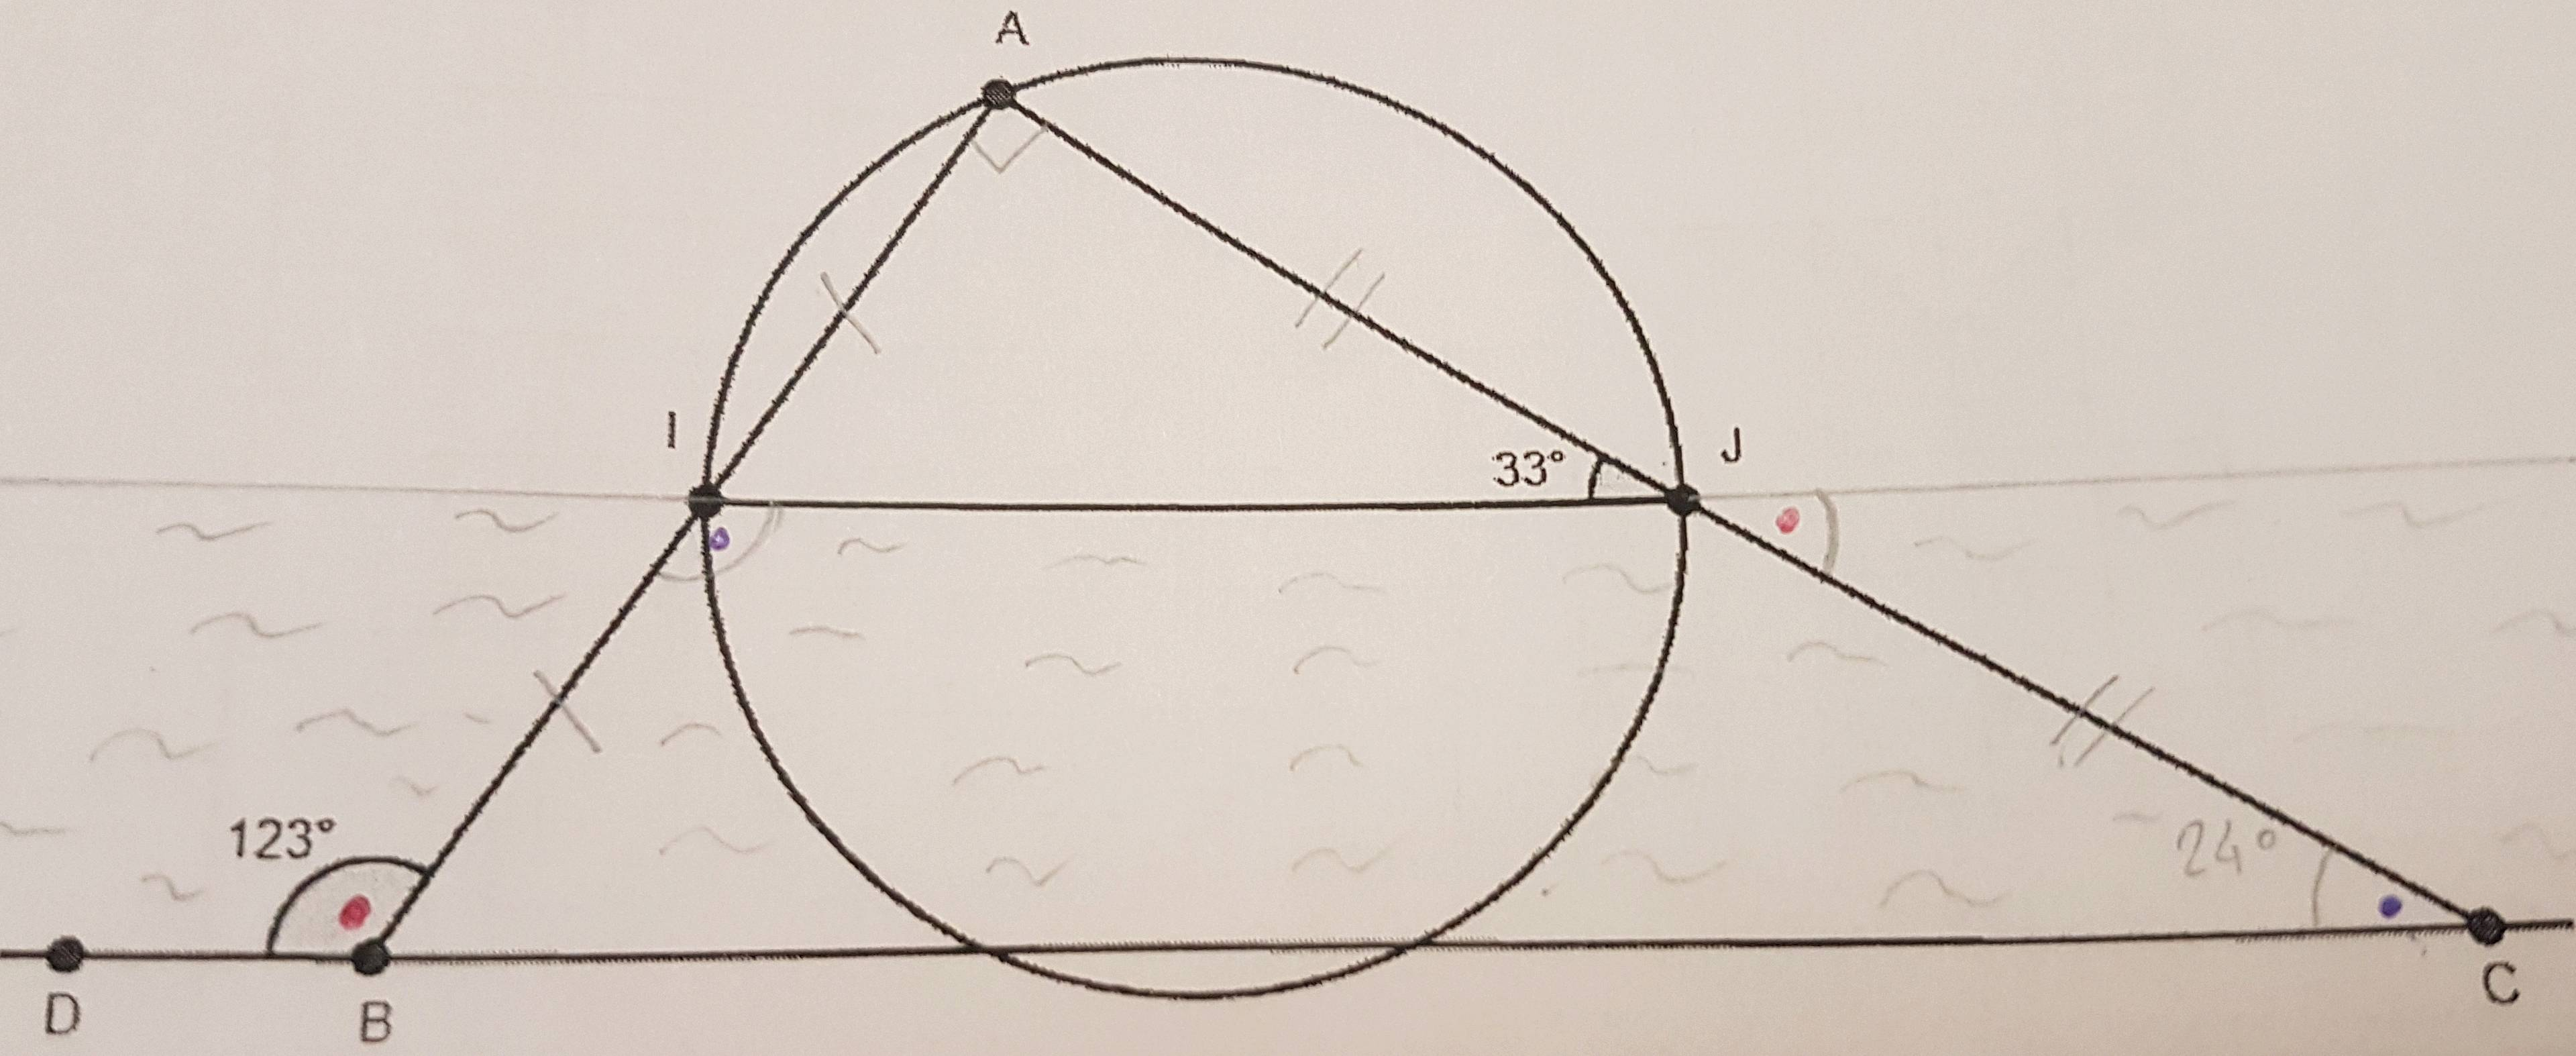
\includegraphics[width=\linewidth]{img/insectes.jpg}
    \caption{Une version évoluée où la coccinelle et la libellule sont schématisées par des points.}
    \label{fig:angles-insecte2}
\end{figure}

\end{appendices}
\end{document}
